\documentclass[twoside]{book}

% Packages required by doxygen
\usepackage{fixltx2e}
\usepackage{calc}
\usepackage{doxygen}
\usepackage[export]{adjustbox} % also loads graphicx
\usepackage{graphicx}
\usepackage[utf8]{inputenc}
\usepackage{makeidx}
\usepackage{multicol}
\usepackage{multirow}
\PassOptionsToPackage{warn}{textcomp}
\usepackage{textcomp}
\usepackage[nointegrals]{wasysym}
\usepackage[table]{xcolor}

% Font selection
\usepackage[T1]{fontenc}
\usepackage[scaled=.90]{helvet}
\usepackage{courier}
\usepackage{amssymb}
\usepackage{sectsty}
\renewcommand{\familydefault}{\sfdefault}
\allsectionsfont{%
  \fontseries{bc}\selectfont%
  \color{darkgray}%
}
\renewcommand{\DoxyLabelFont}{%
  \fontseries{bc}\selectfont%
  \color{darkgray}%
}
\newcommand{\+}{\discretionary{\mbox{\scriptsize$\hookleftarrow$}}{}{}}

% Page & text layout
\usepackage{geometry}
\geometry{%
  a4paper,%
  top=2.5cm,%
  bottom=2.5cm,%
  left=2.5cm,%
  right=2.5cm%
}
\tolerance=750
\hfuzz=15pt
\hbadness=750
\setlength{\emergencystretch}{15pt}
\setlength{\parindent}{0cm}
\setlength{\parskip}{3ex plus 2ex minus 2ex}
\makeatletter
\renewcommand{\paragraph}{%
  \@startsection{paragraph}{4}{0ex}{-1.0ex}{1.0ex}{%
    \normalfont\normalsize\bfseries\SS@parafont%
  }%
}
\renewcommand{\subparagraph}{%
  \@startsection{subparagraph}{5}{0ex}{-1.0ex}{1.0ex}{%
    \normalfont\normalsize\bfseries\SS@subparafont%
  }%
}
\makeatother

% Headers & footers
\usepackage{fancyhdr}
\pagestyle{fancyplain}
\fancyhead[LE]{\fancyplain{}{\bfseries\thepage}}
\fancyhead[CE]{\fancyplain{}{}}
\fancyhead[RE]{\fancyplain{}{\bfseries\leftmark}}
\fancyhead[LO]{\fancyplain{}{\bfseries\rightmark}}
\fancyhead[CO]{\fancyplain{}{}}
\fancyhead[RO]{\fancyplain{}{\bfseries\thepage}}
\fancyfoot[LE]{\fancyplain{}{}}
\fancyfoot[CE]{\fancyplain{}{}}
\fancyfoot[RE]{\fancyplain{}{\bfseries\scriptsize Generated by Doxygen }}
\fancyfoot[LO]{\fancyplain{}{\bfseries\scriptsize Generated by Doxygen }}
\fancyfoot[CO]{\fancyplain{}{}}
\fancyfoot[RO]{\fancyplain{}{}}
\renewcommand{\footrulewidth}{0.4pt}
\renewcommand{\chaptermark}[1]{%
  \markboth{#1}{}%
}
\renewcommand{\sectionmark}[1]{%
  \markright{\thesection\ #1}%
}

% Indices & bibliography
\usepackage{natbib}
\usepackage[titles]{tocloft}
\setcounter{tocdepth}{3}
\setcounter{secnumdepth}{5}
\makeindex

% Hyperlinks (required, but should be loaded last)
\usepackage{ifpdf}
\ifpdf
  \usepackage[pdftex,pagebackref=true]{hyperref}
\else
  \usepackage[ps2pdf,pagebackref=true]{hyperref}
\fi
\hypersetup{%
  colorlinks=true,%
  linkcolor=blue,%
  citecolor=blue,%
  unicode%
}

% Custom commands
\newcommand{\clearemptydoublepage}{%
  \newpage{\pagestyle{empty}\cleardoublepage}%
}

\usepackage{caption}
\captionsetup{labelsep=space,justification=centering,font={bf},singlelinecheck=off,skip=4pt,position=top}

%===== C O N T E N T S =====

\begin{document}

% Titlepage & ToC
\hypersetup{pageanchor=false,
             bookmarksnumbered=true,
             pdfencoding=unicode
            }
\pagenumbering{alph}
\begin{titlepage}
\vspace*{7cm}
\begin{center}%
{\Large The Legend of Python, Modular Interface Specification \\[1ex]\large Revison 2.\+2 12/5/2018 }\\
\vspace*{1cm}
{\large Generated by Doxygen 1.8.13}\\
\end{center}
\end{titlepage}
\clearemptydoublepage
\pagenumbering{roman}
\tableofcontents
\clearemptydoublepage
\pagenumbering{arabic}
\hypersetup{pageanchor=true}

%--- Begin generated contents ---
\chapter{Hierarchical Index}
\section{Class Hierarchy}
This inheritance list is sorted roughly, but not completely, alphabetically\+:\begin{DoxyCompactList}
\item \contentsline{section}{collision.\+levelmanager.\+Level\+Manager}{\pageref{classcollision_1_1levelmanager_1_1_level_manager}}{}
\item object\begin{DoxyCompactList}
\item \contentsline{section}{actor.\+spritesheet.\+Sprite\+Sheet}{\pageref{classactor_1_1spritesheet_1_1_sprite_sheet}}{}
\end{DoxyCompactList}
\item Sprite\begin{DoxyCompactList}
\item \contentsline{section}{actor.\+boomerang.\+Boomerang}{\pageref{classactor_1_1boomerang_1_1_boomerang}}{}
\item \contentsline{section}{actor.\+boss.\+Boss}{\pageref{classactor_1_1boss_1_1_boss}}{}
\begin{DoxyCompactList}
\item \contentsline{section}{actor.\+aquamentus.\+Aquamentus}{\pageref{classactor_1_1aquamentus_1_1_aquamentus}}{}
\end{DoxyCompactList}
\item \contentsline{section}{actor.\+enemy.\+Enemy}{\pageref{classactor_1_1enemy_1_1_enemy}}{}
\begin{DoxyCompactList}
\item \contentsline{section}{actor.\+keese.\+Keese}{\pageref{classactor_1_1keese_1_1_keese}}{}
\item \contentsline{section}{actor.\+stalfos.\+Stalfos}{\pageref{classactor_1_1stalfos_1_1_stalfos}}{}
\end{DoxyCompactList}
\item \contentsline{section}{actor.\+fireball.\+Fireball}{\pageref{classactor_1_1fireball_1_1_fireball}}{}
\item \contentsline{section}{actor.\+healthbar.\+Health\+\_\+\+Bar}{\pageref{classactor_1_1healthbar_1_1_health___bar}}{}
\item \contentsline{section}{actor.\+item.\+Item}{\pageref{classactor_1_1item_1_1_item}}{}
\item \contentsline{section}{actor.\+player.\+Player}{\pageref{classactor_1_1player_1_1_player}}{}
\item \contentsline{section}{actor.\+rupee.\+Rupee\+\_\+\+Bar}{\pageref{classactor_1_1rupee_1_1_rupee___bar}}{}
\item \contentsline{section}{actor.\+sword.\+Sword}{\pageref{classactor_1_1sword_1_1_sword}}{}
\item \contentsline{section}{collision.\+door.\+Door}{\pageref{classcollision_1_1door_1_1_door}}{}
\item \contentsline{section}{collision.\+level.\+Level}{\pageref{classcollision_1_1level_1_1_level}}{}
\item \contentsline{section}{collision.\+wall.\+Wall}{\pageref{classcollision_1_1wall_1_1_wall}}{}
\end{DoxyCompactList}
\end{DoxyCompactList}

\chapter{Class Index}
\section{Class List}
Here are the classes, structs, unions and interfaces with brief descriptions\+:\begin{DoxyCompactList}
\item\contentsline{section}{\hyperlink{classactor_1_1aquamentus_1_1_aquamentus}{actor.\+aquamentus.\+Aquamentus} \\*This class represents the \hyperlink{classactor_1_1aquamentus_1_1_aquamentus}{Aquamentus} Boss }{\pageref{classactor_1_1aquamentus_1_1_aquamentus}}{}
\item\contentsline{section}{\hyperlink{classactor_1_1boomerang_1_1_boomerang}{actor.\+boomerang.\+Boomerang} \\*\hyperlink{classactor_1_1boomerang_1_1_boomerang}{Boomerang} Weapon Class  The class holding the creation, behaviour, and collision effects of the player\textquotesingle{}s boomerang weapon }{\pageref{classactor_1_1boomerang_1_1_boomerang}}{}
\item\contentsline{section}{\hyperlink{classactor_1_1boss_1_1_boss}{actor.\+boss.\+Boss} \\*Superclass for representing a \hyperlink{classactor_1_1boss_1_1_boss}{Boss} }{\pageref{classactor_1_1boss_1_1_boss}}{}
\item\contentsline{section}{\hyperlink{classcollision_1_1door_1_1_door}{collision.\+door.\+Door} \\*Dungeon \hyperlink{classcollision_1_1door_1_1_door}{Door} Class  This class is used to place a door on one of four places of a dungeon room, to allow the player to walk through and traverse to other rooms within the dungeon }{\pageref{classcollision_1_1door_1_1_door}}{}
\item\contentsline{section}{\hyperlink{classactor_1_1enemy_1_1_enemy}{actor.\+enemy.\+Enemy} \\*Superclass for representing an \hyperlink{classactor_1_1enemy_1_1_enemy}{Enemy} }{\pageref{classactor_1_1enemy_1_1_enemy}}{}
\item\contentsline{section}{\hyperlink{classactor_1_1fireball_1_1_fireball}{actor.\+fireball.\+Fireball} \\*This class represents the \hyperlink{classactor_1_1fireball_1_1_fireball}{Fireball} object }{\pageref{classactor_1_1fireball_1_1_fireball}}{}
\item\contentsline{section}{\hyperlink{classactor_1_1healthbar_1_1_health___bar}{actor.\+healthbar.\+Health\+\_\+\+Bar} \\*This class represents the Health\+Bar for the user controlled player character }{\pageref{classactor_1_1healthbar_1_1_health___bar}}{}
\item\contentsline{section}{\hyperlink{classactor_1_1item_1_1_item}{actor.\+item.\+Item} \\*Consumable \hyperlink{classactor_1_1item_1_1_item}{Item} Class  This class is used for the creation of a random consumable item, spawned once an enemy has been defeated on their last position before despawn }{\pageref{classactor_1_1item_1_1_item}}{}
\item\contentsline{section}{\hyperlink{classactor_1_1keese_1_1_keese}{actor.\+keese.\+Keese} \\*This class represents the \hyperlink{classactor_1_1keese_1_1_keese}{Keese} enemy }{\pageref{classactor_1_1keese_1_1_keese}}{}
\item\contentsline{section}{\hyperlink{classcollision_1_1level_1_1_level}{collision.\+level.\+Level} \\*Dungeon level background class  Creates the background of a dungeon, can be modified in the future to change colour based on sprite sheet and new arg }{\pageref{classcollision_1_1level_1_1_level}}{}
\item\contentsline{section}{\hyperlink{classcollision_1_1levelmanager_1_1_level_manager}{collision.\+levelmanager.\+Level\+Manager} \\*Dungeon Level Creation Class  Class used as a master constructor for every dungeon levels, getting pre-\/written data and loading it when the game starts and when a transition occurs }{\pageref{classcollision_1_1levelmanager_1_1_level_manager}}{}
\item\contentsline{section}{\hyperlink{classactor_1_1player_1_1_player}{actor.\+player.\+Player} \\*\hyperlink{classactor_1_1player_1_1_player}{Player} Class  A pygame sprite subclass for defining the creation of the game\textquotesingle{}s playable character, as well as its interactions with both the user and other entities within the game }{\pageref{classactor_1_1player_1_1_player}}{}
\item\contentsline{section}{\hyperlink{classactor_1_1rupee_1_1_rupee___bar}{actor.\+rupee.\+Rupee\+\_\+\+Bar} \\*This class represents the Rupee\+Bar object }{\pageref{classactor_1_1rupee_1_1_rupee___bar}}{}
\item\contentsline{section}{\hyperlink{classactor_1_1spritesheet_1_1_sprite_sheet}{actor.\+spritesheet.\+Sprite\+Sheet} \\*This class represents the \hyperlink{classactor_1_1spritesheet_1_1_sprite_sheet}{Sprite\+Sheet} object, allowing sprites to be loaded and processed }{\pageref{classactor_1_1spritesheet_1_1_sprite_sheet}}{}
\item\contentsline{section}{\hyperlink{classactor_1_1stalfos_1_1_stalfos}{actor.\+stalfos.\+Stalfos} \\*This class represents the \hyperlink{classactor_1_1stalfos_1_1_stalfos}{Stalfos} enemy }{\pageref{classactor_1_1stalfos_1_1_stalfos}}{}
\item\contentsline{section}{\hyperlink{classactor_1_1sword_1_1_sword}{actor.\+sword.\+Sword} \\*Player \hyperlink{classactor_1_1sword_1_1_sword}{Sword} Class  Class for the creation and deletion of the sword sprite object, made when the player attacks }{\pageref{classactor_1_1sword_1_1_sword}}{}
\item\contentsline{section}{\hyperlink{classcollision_1_1wall_1_1_wall}{collision.\+wall.\+Wall} \\*This class represents the \hyperlink{classcollision_1_1wall_1_1_wall}{Wall} class for collision for objects in the environment }{\pageref{classcollision_1_1wall_1_1_wall}}{}
\end{DoxyCompactList}

\chapter{File Index}
\section{File List}
Here is a list of all documented files with brief descriptions\+:\begin{DoxyCompactList}
\item\contentsline{section}{src/actor/\hyperlink{aquamentus_8py}{aquamentus.\+py} \\*Aquamentus Boss }{\pageref{aquamentus_8py}}{}
\item\contentsline{section}{src/actor/\hyperlink{boomerang_8py}{boomerang.\+py} \\*Boomerang Weapon }{\pageref{boomerang_8py}}{}
\item\contentsline{section}{src/actor/\hyperlink{boss_8py}{boss.\+py} \\*Boss Template }{\pageref{boss_8py}}{}
\item\contentsline{section}{src/actor/\hyperlink{constants_8py}{constants.\+py} \\*Actor Constants }{\pageref{constants_8py}}{}
\item\contentsline{section}{src/actor/\hyperlink{enemy_8py}{enemy.\+py} \\*Enemy Template }{\pageref{enemy_8py}}{}
\item\contentsline{section}{src/actor/\hyperlink{fireball_8py}{fireball.\+py} \\*Fireball object }{\pageref{fireball_8py}}{}
\item\contentsline{section}{src/actor/\hyperlink{healthbar_8py}{healthbar.\+py} \\*Health\+Bar Class }{\pageref{healthbar_8py}}{}
\item\contentsline{section}{src/actor/\hyperlink{item_8py}{item.\+py} \\*Consumable Items }{\pageref{item_8py}}{}
\item\contentsline{section}{src/actor/\hyperlink{keese_8py}{keese.\+py} \\*Keese Enemy }{\pageref{keese_8py}}{}
\item\contentsline{section}{src/actor/\hyperlink{player_8py}{player.\+py} \\*Playable Characer }{\pageref{player_8py}}{}
\item\contentsline{section}{src/actor/\hyperlink{rupee_8py}{rupee.\+py} \\*Rupee\+\_\+\+Bar Class }{\pageref{rupee_8py}}{}
\item\contentsline{section}{src/actor/\hyperlink{spritesheet_8py}{spritesheet.\+py} \\*Sprite\+Sheet Class }{\pageref{spritesheet_8py}}{}
\item\contentsline{section}{src/actor/\hyperlink{stalfos_8py}{stalfos.\+py} \\*Stalfos Enemy }{\pageref{stalfos_8py}}{}
\item\contentsline{section}{src/actor/\hyperlink{sword_8py}{sword.\+py} \\*Player Sword }{\pageref{sword_8py}}{}
\item\contentsline{section}{src/collision/\hyperlink{door_8py}{door.\+py} \\*Dungeon Door }{\pageref{door_8py}}{}
\item\contentsline{section}{src/collision/\hyperlink{level_8py}{level.\+py} \\*Dungeon Background }{\pageref{level_8py}}{}
\item\contentsline{section}{src/collision/\hyperlink{levelmanager_8py}{levelmanager.\+py} \\*Dungeon Level Master Creator }{\pageref{levelmanager_8py}}{}
\item\contentsline{section}{src/collision/\hyperlink{wall_8py}{wall.\+py} \\*Wall Class }{\pageref{wall_8py}}{}
\item\contentsline{section}{src/config/\hyperlink{colour_8py}{colour.\+py} \\*Colour Constants }{\pageref{colour_8py}}{}
\item\contentsline{section}{src/config/\hyperlink{window_8py}{window.\+py} \\*Window Constants }{\pageref{window_8py}}{}
\end{DoxyCompactList}

\chapter{Class Documentation}
\hypertarget{classactor_1_1aquamentus_1_1_aquamentus}{}\section{actor.\+aquamentus.\+Aquamentus Class Reference}
\label{classactor_1_1aquamentus_1_1_aquamentus}\index{actor.\+aquamentus.\+Aquamentus@{actor.\+aquamentus.\+Aquamentus}}


This class represents the \hyperlink{classactor_1_1aquamentus_1_1_aquamentus}{Aquamentus} Boss.  


Inheritance diagram for actor.\+aquamentus.\+Aquamentus\+:\begin{figure}[H]
\begin{center}
\leavevmode
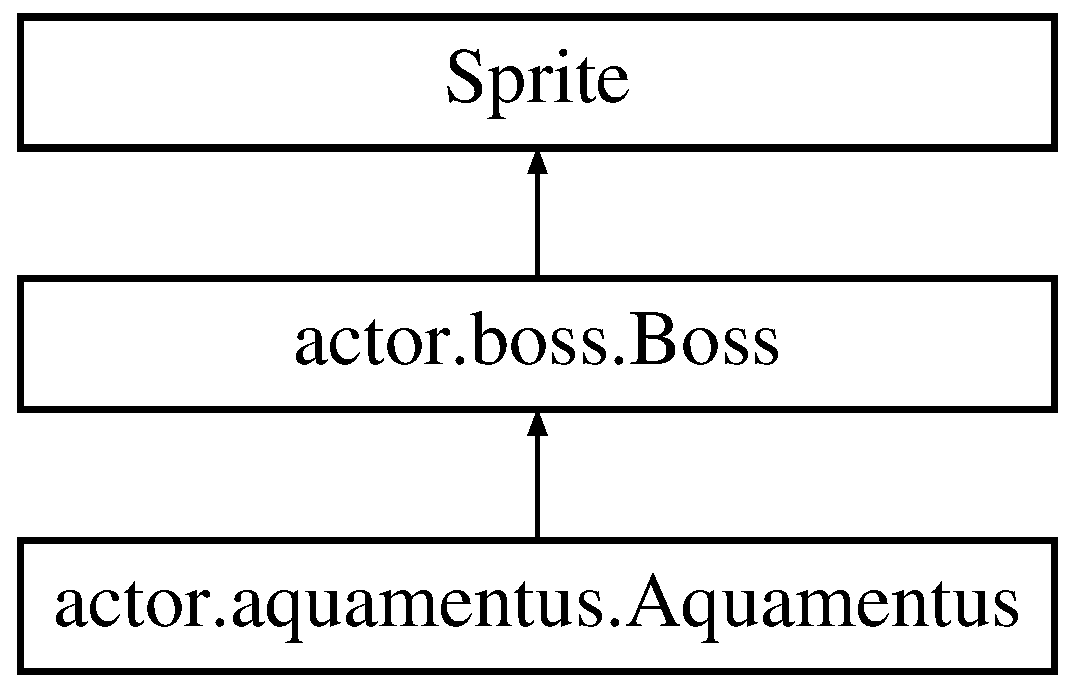
\includegraphics[height=3.000000cm]{classactor_1_1aquamentus_1_1_aquamentus}
\end{center}
\end{figure}
\subsection*{Public Member Functions}
\begin{DoxyCompactItemize}
\item 
def \hyperlink{classactor_1_1aquamentus_1_1_aquamentus_a410081eed92439a0429ea0fb75eb2328}{\+\_\+\+\_\+init\+\_\+\+\_\+} (self, x, y)
\begin{DoxyCompactList}\small\item\em Constructor for \hyperlink{classactor_1_1aquamentus_1_1_aquamentus}{Aquamentus}. \end{DoxyCompactList}\item 
def \hyperlink{classactor_1_1aquamentus_1_1_aquamentus_a9a995cf75da6e464cf0292c7514536e5}{check\+State} (self)
\begin{DoxyCompactList}\small\item\em Evaluates the state of the \hyperlink{classactor_1_1aquamentus_1_1_aquamentus}{Aquamentus}. \end{DoxyCompactList}\item 
def \hyperlink{classactor_1_1aquamentus_1_1_aquamentus_a63dc79ec42118be2c34462ea5fdcbade}{swap\+Direction} (self)
\begin{DoxyCompactList}\small\item\em Swaps \hyperlink{classactor_1_1aquamentus_1_1_aquamentus}{Aquamentus}\textquotesingle{} direction. \end{DoxyCompactList}\item 
def \hyperlink{classactor_1_1aquamentus_1_1_aquamentus_a8cd94900aed592550a65f7761a6331bb}{attack} (self)
\begin{DoxyCompactList}\small\item\em Allows for \hyperlink{classactor_1_1aquamentus_1_1_aquamentus}{Aquamentus} to attack. \end{DoxyCompactList}\item 
def \hyperlink{classactor_1_1aquamentus_1_1_aquamentus_a5569e3e099e8754db819fe31e893bb6f}{boss\+Logic} (self)
\begin{DoxyCompactList}\small\item\em Controls \hyperlink{classactor_1_1aquamentus_1_1_aquamentus}{Aquamentus} logic. \end{DoxyCompactList}\end{DoxyCompactItemize}
\subsection*{Public Attributes}
\begin{DoxyCompactItemize}
\item 
\mbox{\Hypertarget{classactor_1_1aquamentus_1_1_aquamentus_ad37d613a7b0aff59695801ed84691959}\label{classactor_1_1aquamentus_1_1_aquamentus_ad37d613a7b0aff59695801ed84691959}} 
\hyperlink{classactor_1_1aquamentus_1_1_aquamentus_ad37d613a7b0aff59695801ed84691959}{is\+Attacking}
\begin{DoxyCompactList}\small\item\em Represents wether or not the boss is attacking. \end{DoxyCompactList}\item 
\mbox{\Hypertarget{classactor_1_1aquamentus_1_1_aquamentus_adc3d75725497270071e563121cb687e2}\label{classactor_1_1aquamentus_1_1_aquamentus_adc3d75725497270071e563121cb687e2}} 
\hyperlink{classactor_1_1aquamentus_1_1_aquamentus_adc3d75725497270071e563121cb687e2}{attack\+Start\+Frame}
\begin{DoxyCompactList}\small\item\em Represents the frame that the boss starts an attack. \end{DoxyCompactList}\item 
\mbox{\Hypertarget{classactor_1_1aquamentus_1_1_aquamentus_a3789eb3b652e8956c8215c444416de8c}\label{classactor_1_1aquamentus_1_1_aquamentus_a3789eb3b652e8956c8215c444416de8c}} 
\hyperlink{classactor_1_1aquamentus_1_1_aquamentus_a3789eb3b652e8956c8215c444416de8c}{fireballs}
\begin{DoxyCompactList}\small\item\em Represents the boss\textquotesingle{} fireballs. \end{DoxyCompactList}\item 
\mbox{\Hypertarget{classactor_1_1aquamentus_1_1_aquamentus_a72a68cb13edf22766de1bb935d77b477}\label{classactor_1_1aquamentus_1_1_aquamentus_a72a68cb13edf22766de1bb935d77b477}} 
\hyperlink{classactor_1_1aquamentus_1_1_aquamentus_a72a68cb13edf22766de1bb935d77b477}{x\+Speed}
\begin{DoxyCompactList}\small\item\em \hyperlink{classactor_1_1aquamentus_1_1_aquamentus}{Aquamentus}\textquotesingle{} set x speed. \end{DoxyCompactList}\item 
\mbox{\Hypertarget{classactor_1_1aquamentus_1_1_aquamentus_a590144e96f88385400ac90281bb281c8}\label{classactor_1_1aquamentus_1_1_aquamentus_a590144e96f88385400ac90281bb281c8}} 
\hyperlink{classactor_1_1aquamentus_1_1_aquamentus_a590144e96f88385400ac90281bb281c8}{max\+HP}
\begin{DoxyCompactList}\small\item\em \hyperlink{classactor_1_1aquamentus_1_1_aquamentus}{Aquamentus}\textquotesingle{} max health. \end{DoxyCompactList}\item 
\mbox{\Hypertarget{classactor_1_1aquamentus_1_1_aquamentus_a53a55e5f5a79a7cf81bf9833527e0e78}\label{classactor_1_1aquamentus_1_1_aquamentus_a53a55e5f5a79a7cf81bf9833527e0e78}} 
\hyperlink{classactor_1_1aquamentus_1_1_aquamentus_a53a55e5f5a79a7cf81bf9833527e0e78}{HP}
\begin{DoxyCompactList}\small\item\em \hyperlink{classactor_1_1aquamentus_1_1_aquamentus}{Aquamentus}\textquotesingle{} current health. \end{DoxyCompactList}\item 
\mbox{\Hypertarget{classactor_1_1aquamentus_1_1_aquamentus_a07199a4ba31b82aabf858080155c0ba9}\label{classactor_1_1aquamentus_1_1_aquamentus_a07199a4ba31b82aabf858080155c0ba9}} 
\hyperlink{classactor_1_1aquamentus_1_1_aquamentus_a07199a4ba31b82aabf858080155c0ba9}{dmg}
\begin{DoxyCompactList}\small\item\em \hyperlink{classactor_1_1aquamentus_1_1_aquamentus}{Aquamentus}\textquotesingle{} damage. \end{DoxyCompactList}\item 
\mbox{\Hypertarget{classactor_1_1aquamentus_1_1_aquamentus_a565189024813dd0a1ad6c4fd1d89ac31}\label{classactor_1_1aquamentus_1_1_aquamentus_a565189024813dd0a1ad6c4fd1d89ac31}} 
\hyperlink{classactor_1_1aquamentus_1_1_aquamentus_a565189024813dd0a1ad6c4fd1d89ac31}{image}
\begin{DoxyCompactList}\small\item\em Sprite image. \end{DoxyCompactList}\item 
\mbox{\Hypertarget{classactor_1_1aquamentus_1_1_aquamentus_a725395188c0754812edd9c26595f5c25}\label{classactor_1_1aquamentus_1_1_aquamentus_a725395188c0754812edd9c26595f5c25}} 
\hyperlink{classactor_1_1aquamentus_1_1_aquamentus_a725395188c0754812edd9c26595f5c25}{sprites}
\begin{DoxyCompactList}\small\item\em Array of sprites. \end{DoxyCompactList}\item 
\mbox{\Hypertarget{classactor_1_1aquamentus_1_1_aquamentus_a66f41eed56eff4a71e1bd191fa401afc}\label{classactor_1_1aquamentus_1_1_aquamentus_a66f41eed56eff4a71e1bd191fa401afc}} 
\hyperlink{classactor_1_1aquamentus_1_1_aquamentus_a66f41eed56eff4a71e1bd191fa401afc}{obj}
\begin{DoxyCompactList}\small\item\em Collision list. \end{DoxyCompactList}\item 
\mbox{\Hypertarget{classactor_1_1aquamentus_1_1_aquamentus_a7b369f65489176836b8f7108419f17a4}\label{classactor_1_1aquamentus_1_1_aquamentus_a7b369f65489176836b8f7108419f17a4}} 
\hyperlink{classactor_1_1aquamentus_1_1_aquamentus_a7b369f65489176836b8f7108419f17a4}{sprite\+Index}
\begin{DoxyCompactList}\small\item\em Index for the array of sprites. \end{DoxyCompactList}\item 
\hyperlink{classactor_1_1aquamentus_1_1_aquamentus_ade0294266872c152be5a7ae1c1b14fc6}{hit\+Count}
\begin{DoxyCompactList}\small\item\em Integer value representing the buffer for the number of hits for \hyperlink{classactor_1_1aquamentus_1_1_aquamentus}{Aquamentus} after being hit by player character. \end{DoxyCompactList}\item 
\hyperlink{classactor_1_1aquamentus_1_1_aquamentus_a6acef447408a84f5af003f3cf74dec7c}{is\+Hit}
\begin{DoxyCompactList}\small\item\em Represents the current state if \hyperlink{classactor_1_1aquamentus_1_1_aquamentus}{Aquamentus} has collided with player character attack. \end{DoxyCompactList}\item 
\hyperlink{classactor_1_1aquamentus_1_1_aquamentus_a462a8a223836cc3b1154ba73cbcd4703}{oldx}
\begin{DoxyCompactList}\small\item\em This represents the previous x-\/location of \hyperlink{classactor_1_1aquamentus_1_1_aquamentus}{Aquamentus} in movement/stationary state. \end{DoxyCompactList}\item 
\hyperlink{classactor_1_1aquamentus_1_1_aquamentus_a985f847ed6c6df6d09232a42f8263b8c}{oldy}
\begin{DoxyCompactList}\small\item\em This represents the previous y-\/location of \hyperlink{classactor_1_1aquamentus_1_1_aquamentus}{Aquamentus} in movement/stationary state. \end{DoxyCompactList}\end{DoxyCompactItemize}


\subsection{Detailed Description}
This class represents the \hyperlink{classactor_1_1aquamentus_1_1_aquamentus}{Aquamentus} Boss. 

\subsection{Constructor \& Destructor Documentation}
\mbox{\Hypertarget{classactor_1_1aquamentus_1_1_aquamentus_a410081eed92439a0429ea0fb75eb2328}\label{classactor_1_1aquamentus_1_1_aquamentus_a410081eed92439a0429ea0fb75eb2328}} 
\index{actor\+::aquamentus\+::\+Aquamentus@{actor\+::aquamentus\+::\+Aquamentus}!\+\_\+\+\_\+init\+\_\+\+\_\+@{\+\_\+\+\_\+init\+\_\+\+\_\+}}
\index{\+\_\+\+\_\+init\+\_\+\+\_\+@{\+\_\+\+\_\+init\+\_\+\+\_\+}!actor\+::aquamentus\+::\+Aquamentus@{actor\+::aquamentus\+::\+Aquamentus}}
\subsubsection{\texorpdfstring{\+\_\+\+\_\+init\+\_\+\+\_\+()}{\_\_init\_\_()}}
{\footnotesize\ttfamily def actor.\+aquamentus.\+Aquamentus.\+\_\+\+\_\+init\+\_\+\+\_\+ (\begin{DoxyParamCaption}\item[{}]{self,  }\item[{}]{x,  }\item[{}]{y }\end{DoxyParamCaption})}



Constructor for \hyperlink{classactor_1_1aquamentus_1_1_aquamentus}{Aquamentus}. 

Constructor takes two parameters, the x and y coordinates 
\begin{DoxyParams}{Parameters}
{\em x} & X coordinate of the starting postion of the \hyperlink{classactor_1_1aquamentus_1_1_aquamentus}{Aquamentus} \\
\hline
{\em y} & Y coordinate of the starting postion of the \hyperlink{classactor_1_1aquamentus_1_1_aquamentus}{Aquamentus} \\
\hline
\end{DoxyParams}


\subsection{Member Function Documentation}
\mbox{\Hypertarget{classactor_1_1aquamentus_1_1_aquamentus_a8cd94900aed592550a65f7761a6331bb}\label{classactor_1_1aquamentus_1_1_aquamentus_a8cd94900aed592550a65f7761a6331bb}} 
\index{actor\+::aquamentus\+::\+Aquamentus@{actor\+::aquamentus\+::\+Aquamentus}!attack@{attack}}
\index{attack@{attack}!actor\+::aquamentus\+::\+Aquamentus@{actor\+::aquamentus\+::\+Aquamentus}}
\subsubsection{\texorpdfstring{attack()}{attack()}}
{\footnotesize\ttfamily def actor.\+aquamentus.\+Aquamentus.\+attack (\begin{DoxyParamCaption}\item[{}]{self }\end{DoxyParamCaption})}



Allows for \hyperlink{classactor_1_1aquamentus_1_1_aquamentus}{Aquamentus} to attack. 

Spawns fireballs at Aquamenuts\textquotesingle{} mouth and sets their move speed \mbox{\Hypertarget{classactor_1_1aquamentus_1_1_aquamentus_a5569e3e099e8754db819fe31e893bb6f}\label{classactor_1_1aquamentus_1_1_aquamentus_a5569e3e099e8754db819fe31e893bb6f}} 
\index{actor\+::aquamentus\+::\+Aquamentus@{actor\+::aquamentus\+::\+Aquamentus}!boss\+Logic@{boss\+Logic}}
\index{boss\+Logic@{boss\+Logic}!actor\+::aquamentus\+::\+Aquamentus@{actor\+::aquamentus\+::\+Aquamentus}}
\subsubsection{\texorpdfstring{boss\+Logic()}{bossLogic()}}
{\footnotesize\ttfamily def actor.\+aquamentus.\+Aquamentus.\+boss\+Logic (\begin{DoxyParamCaption}\item[{}]{self }\end{DoxyParamCaption})}



Controls \hyperlink{classactor_1_1aquamentus_1_1_aquamentus}{Aquamentus} logic. 

Uses the states to control the \hyperlink{classactor_1_1aquamentus_1_1_aquamentus}{Aquamentus} \mbox{\Hypertarget{classactor_1_1aquamentus_1_1_aquamentus_a9a995cf75da6e464cf0292c7514536e5}\label{classactor_1_1aquamentus_1_1_aquamentus_a9a995cf75da6e464cf0292c7514536e5}} 
\index{actor\+::aquamentus\+::\+Aquamentus@{actor\+::aquamentus\+::\+Aquamentus}!check\+State@{check\+State}}
\index{check\+State@{check\+State}!actor\+::aquamentus\+::\+Aquamentus@{actor\+::aquamentus\+::\+Aquamentus}}
\subsubsection{\texorpdfstring{check\+State()}{checkState()}}
{\footnotesize\ttfamily def actor.\+aquamentus.\+Aquamentus.\+check\+State (\begin{DoxyParamCaption}\item[{}]{self }\end{DoxyParamCaption})}



Evaluates the state of the \hyperlink{classactor_1_1aquamentus_1_1_aquamentus}{Aquamentus}. 

Evalautes if \hyperlink{classactor_1_1aquamentus_1_1_aquamentus}{Aquamentus} can stop, if it is in iframes, if it collides with something, and if it has died \mbox{\Hypertarget{classactor_1_1aquamentus_1_1_aquamentus_a63dc79ec42118be2c34462ea5fdcbade}\label{classactor_1_1aquamentus_1_1_aquamentus_a63dc79ec42118be2c34462ea5fdcbade}} 
\index{actor\+::aquamentus\+::\+Aquamentus@{actor\+::aquamentus\+::\+Aquamentus}!swap\+Direction@{swap\+Direction}}
\index{swap\+Direction@{swap\+Direction}!actor\+::aquamentus\+::\+Aquamentus@{actor\+::aquamentus\+::\+Aquamentus}}
\subsubsection{\texorpdfstring{swap\+Direction()}{swapDirection()}}
{\footnotesize\ttfamily def actor.\+aquamentus.\+Aquamentus.\+swap\+Direction (\begin{DoxyParamCaption}\item[{}]{self }\end{DoxyParamCaption})}



Swaps \hyperlink{classactor_1_1aquamentus_1_1_aquamentus}{Aquamentus}\textquotesingle{} direction. 

Multiplies the speed in the x direction by -\/1 

\subsection{Member Data Documentation}
\mbox{\Hypertarget{classactor_1_1aquamentus_1_1_aquamentus_ade0294266872c152be5a7ae1c1b14fc6}\label{classactor_1_1aquamentus_1_1_aquamentus_ade0294266872c152be5a7ae1c1b14fc6}} 
\index{actor\+::aquamentus\+::\+Aquamentus@{actor\+::aquamentus\+::\+Aquamentus}!hit\+Count@{hit\+Count}}
\index{hit\+Count@{hit\+Count}!actor\+::aquamentus\+::\+Aquamentus@{actor\+::aquamentus\+::\+Aquamentus}}
\subsubsection{\texorpdfstring{hit\+Count}{hitCount}}
{\footnotesize\ttfamily actor.\+aquamentus.\+Aquamentus.\+hit\+Count}



Integer value representing the buffer for the number of hits for \hyperlink{classactor_1_1aquamentus_1_1_aquamentus}{Aquamentus} after being hit by player character. 

\mbox{\Hypertarget{classactor_1_1aquamentus_1_1_aquamentus_a6acef447408a84f5af003f3cf74dec7c}\label{classactor_1_1aquamentus_1_1_aquamentus_a6acef447408a84f5af003f3cf74dec7c}} 
\index{actor\+::aquamentus\+::\+Aquamentus@{actor\+::aquamentus\+::\+Aquamentus}!is\+Hit@{is\+Hit}}
\index{is\+Hit@{is\+Hit}!actor\+::aquamentus\+::\+Aquamentus@{actor\+::aquamentus\+::\+Aquamentus}}
\subsubsection{\texorpdfstring{is\+Hit}{isHit}}
{\footnotesize\ttfamily actor.\+aquamentus.\+Aquamentus.\+is\+Hit}



Represents the current state if \hyperlink{classactor_1_1aquamentus_1_1_aquamentus}{Aquamentus} has collided with player character attack. 

\mbox{\Hypertarget{classactor_1_1aquamentus_1_1_aquamentus_a462a8a223836cc3b1154ba73cbcd4703}\label{classactor_1_1aquamentus_1_1_aquamentus_a462a8a223836cc3b1154ba73cbcd4703}} 
\index{actor\+::aquamentus\+::\+Aquamentus@{actor\+::aquamentus\+::\+Aquamentus}!oldx@{oldx}}
\index{oldx@{oldx}!actor\+::aquamentus\+::\+Aquamentus@{actor\+::aquamentus\+::\+Aquamentus}}
\subsubsection{\texorpdfstring{oldx}{oldx}}
{\footnotesize\ttfamily actor.\+aquamentus.\+Aquamentus.\+oldx}



This represents the previous x-\/location of \hyperlink{classactor_1_1aquamentus_1_1_aquamentus}{Aquamentus} in movement/stationary state. 

\mbox{\Hypertarget{classactor_1_1aquamentus_1_1_aquamentus_a985f847ed6c6df6d09232a42f8263b8c}\label{classactor_1_1aquamentus_1_1_aquamentus_a985f847ed6c6df6d09232a42f8263b8c}} 
\index{actor\+::aquamentus\+::\+Aquamentus@{actor\+::aquamentus\+::\+Aquamentus}!oldy@{oldy}}
\index{oldy@{oldy}!actor\+::aquamentus\+::\+Aquamentus@{actor\+::aquamentus\+::\+Aquamentus}}
\subsubsection{\texorpdfstring{oldy}{oldy}}
{\footnotesize\ttfamily actor.\+aquamentus.\+Aquamentus.\+oldy}



This represents the previous y-\/location of \hyperlink{classactor_1_1aquamentus_1_1_aquamentus}{Aquamentus} in movement/stationary state. 



The documentation for this class was generated from the following file\+:\begin{DoxyCompactItemize}
\item 
src/actor/\hyperlink{aquamentus_8py}{aquamentus.\+py}\end{DoxyCompactItemize}

\hypertarget{classactor_1_1boomerang_1_1_boomerang}{}\section{actor.\+boomerang.\+Boomerang Class Reference}
\label{classactor_1_1boomerang_1_1_boomerang}\index{actor.\+boomerang.\+Boomerang@{actor.\+boomerang.\+Boomerang}}


\hyperlink{classactor_1_1boomerang_1_1_boomerang}{Boomerang} Weapon Class  The class holding the creation, behaviour, and collision effects of the player\textquotesingle{}s boomerang weapon.  


Inheritance diagram for actor.\+boomerang.\+Boomerang\+:\begin{figure}[H]
\begin{center}
\leavevmode
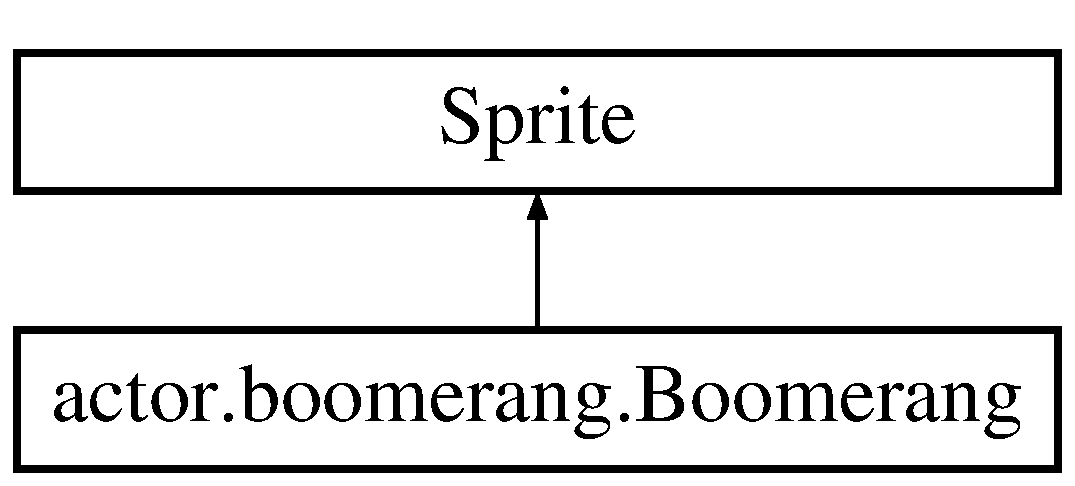
\includegraphics[height=2.000000cm]{classactor_1_1boomerang_1_1_boomerang}
\end{center}
\end{figure}
\subsection*{Public Member Functions}
\begin{DoxyCompactItemize}
\item 
def \hyperlink{classactor_1_1boomerang_1_1_boomerang_a7b20570fa9c54aaba3623075f99770f1}{\+\_\+\+\_\+init\+\_\+\+\_\+} (self, x, y, direction, \hyperlink{classactor_1_1boomerang_1_1_boomerang_a3f28b182298ed6f753bbaa2bacc50287}{obj}, player)
\begin{DoxyCompactList}\small\item\em \hyperlink{classactor_1_1boomerang_1_1_boomerang}{Boomerang} constructor  A sprite subclass constructor that takes an x and y position (the players), a direction for the boomerang\textquotesingle{}s trajectory, a list of collidable objects, as well as the player object (to add to the collision list) \end{DoxyCompactList}\item 
\mbox{\Hypertarget{classactor_1_1boomerang_1_1_boomerang_a5a0f0c1b4d25b5fa10ecb7b02a4f6b5e}\label{classactor_1_1boomerang_1_1_boomerang_a5a0f0c1b4d25b5fa10ecb7b02a4f6b5e}} 
def \hyperlink{classactor_1_1boomerang_1_1_boomerang_a5a0f0c1b4d25b5fa10ecb7b02a4f6b5e}{moveupdate} (self)
\begin{DoxyCompactList}\small\item\em \hyperlink{classactor_1_1boomerang_1_1_boomerang}{Boomerang} position updating function, updating position based on changing trajectory speed. \end{DoxyCompactList}\item 
\mbox{\Hypertarget{classactor_1_1boomerang_1_1_boomerang_abbfebdf98803c7e4ac69a1a6e251d781}\label{classactor_1_1boomerang_1_1_boomerang_abbfebdf98803c7e4ac69a1a6e251d781}} 
def \hyperlink{classactor_1_1boomerang_1_1_boomerang_abbfebdf98803c7e4ac69a1a6e251d781}{collisionupdate} (self)
\begin{DoxyCompactList}\small\item\em \hyperlink{classactor_1_1boomerang_1_1_boomerang}{Boomerang} collision updating function, constantly checking for collisions and acting accordingly. \end{DoxyCompactList}\item 
\mbox{\Hypertarget{classactor_1_1boomerang_1_1_boomerang_a8ed616f57acf720fdd4d7bd5702e1684}\label{classactor_1_1boomerang_1_1_boomerang_a8ed616f57acf720fdd4d7bd5702e1684}} 
def \hyperlink{classactor_1_1boomerang_1_1_boomerang_a8ed616f57acf720fdd4d7bd5702e1684}{spriteupdate} (self)
\begin{DoxyCompactList}\small\item\em Updates the boomerang sprite every 10 frames. \end{DoxyCompactList}\item 
\mbox{\Hypertarget{classactor_1_1boomerang_1_1_boomerang_a5e84fc23d586483105c71cc4c607264c}\label{classactor_1_1boomerang_1_1_boomerang_a5e84fc23d586483105c71cc4c607264c}} 
def \hyperlink{classactor_1_1boomerang_1_1_boomerang_a5e84fc23d586483105c71cc4c607264c}{update} (self)
\begin{DoxyCompactList}\small\item\em \hyperlink{classactor_1_1boomerang_1_1_boomerang}{Boomerang} updating function, repeatedly running moveupdate and collisionupdate. \end{DoxyCompactList}\item 
\mbox{\Hypertarget{classactor_1_1boomerang_1_1_boomerang_ad32ffa27cd6221ed74d144f8874eae5f}\label{classactor_1_1boomerang_1_1_boomerang_ad32ffa27cd6221ed74d144f8874eae5f}} 
def \hyperlink{classactor_1_1boomerang_1_1_boomerang_ad32ffa27cd6221ed74d144f8874eae5f}{collision} (self)
\begin{DoxyCompactList}\small\item\em Default collision function to satisfy other class collision calls to this object. \end{DoxyCompactList}\end{DoxyCompactItemize}
\subsection*{Public Attributes}
\begin{DoxyCompactItemize}
\item 
\mbox{\Hypertarget{classactor_1_1boomerang_1_1_boomerang_afff9077b183225033461cc14dede928b}\label{classactor_1_1boomerang_1_1_boomerang_afff9077b183225033461cc14dede928b}} 
\hyperlink{classactor_1_1boomerang_1_1_boomerang_afff9077b183225033461cc14dede928b}{image}
\begin{DoxyCompactList}\small\item\em \hyperlink{classactor_1_1boomerang_1_1_boomerang}{Boomerang} sprite image. \end{DoxyCompactList}\item 
\mbox{\Hypertarget{classactor_1_1boomerang_1_1_boomerang_a46ad11df1efc1a8395a6bff47b34308f}\label{classactor_1_1boomerang_1_1_boomerang_a46ad11df1efc1a8395a6bff47b34308f}} 
\hyperlink{classactor_1_1boomerang_1_1_boomerang_a46ad11df1efc1a8395a6bff47b34308f}{rect}
\begin{DoxyCompactList}\small\item\em Position of boomerang. \end{DoxyCompactList}\item 
\mbox{\Hypertarget{classactor_1_1boomerang_1_1_boomerang_abd6b4b22c63a81db76e468ec0da228b3}\label{classactor_1_1boomerang_1_1_boomerang_abd6b4b22c63a81db76e468ec0da228b3}} 
\hyperlink{classactor_1_1boomerang_1_1_boomerang_abd6b4b22c63a81db76e468ec0da228b3}{dir}
\begin{DoxyCompactList}\small\item\em Initial travel direction of boomerang. \end{DoxyCompactList}\item 
\mbox{\Hypertarget{classactor_1_1boomerang_1_1_boomerang_a67772200ff4603844c7941f8be87947f}\label{classactor_1_1boomerang_1_1_boomerang_a67772200ff4603844c7941f8be87947f}} 
\hyperlink{classactor_1_1boomerang_1_1_boomerang_a67772200ff4603844c7941f8be87947f}{speed}
\begin{DoxyCompactList}\small\item\em \hyperlink{classactor_1_1boomerang_1_1_boomerang}{Boomerang} initial update speed. \end{DoxyCompactList}\item 
\mbox{\Hypertarget{classactor_1_1boomerang_1_1_boomerang_a3f28b182298ed6f753bbaa2bacc50287}\label{classactor_1_1boomerang_1_1_boomerang_a3f28b182298ed6f753bbaa2bacc50287}} 
\hyperlink{classactor_1_1boomerang_1_1_boomerang_a3f28b182298ed6f753bbaa2bacc50287}{obj}
\begin{DoxyCompactList}\small\item\em List of objects the boomerang could collide with. \end{DoxyCompactList}\item 
\mbox{\Hypertarget{classactor_1_1boomerang_1_1_boomerang_abfb405ccedae18b49b36d5504a548aed}\label{classactor_1_1boomerang_1_1_boomerang_abfb405ccedae18b49b36d5504a548aed}} 
\hyperlink{classactor_1_1boomerang_1_1_boomerang_abfb405ccedae18b49b36d5504a548aed}{killable}
\begin{DoxyCompactList}\small\item\em Boolean to tell when the boomerang should be deleted. \end{DoxyCompactList}\item 
\mbox{\Hypertarget{classactor_1_1boomerang_1_1_boomerang_a54e828173053f349639a8e75b56281c6}\label{classactor_1_1boomerang_1_1_boomerang_a54e828173053f349639a8e75b56281c6}} 
\hyperlink{classactor_1_1boomerang_1_1_boomerang_a54e828173053f349639a8e75b56281c6}{sprites}
\begin{DoxyCompactList}\small\item\em List of sprites for boomerang. \end{DoxyCompactList}\item 
\mbox{\Hypertarget{classactor_1_1boomerang_1_1_boomerang_affb047b1f34deb8f68d0d6d5ee499429}\label{classactor_1_1boomerang_1_1_boomerang_affb047b1f34deb8f68d0d6d5ee499429}} 
\hyperlink{classactor_1_1boomerang_1_1_boomerang_affb047b1f34deb8f68d0d6d5ee499429}{sprite\+Index}
\begin{DoxyCompactList}\small\item\em Index of the current sprite. \end{DoxyCompactList}\item 
\mbox{\Hypertarget{classactor_1_1boomerang_1_1_boomerang_ae815f4dbc9a5e7c3d8e4596c41001c70}\label{classactor_1_1boomerang_1_1_boomerang_ae815f4dbc9a5e7c3d8e4596c41001c70}} 
\hyperlink{classactor_1_1boomerang_1_1_boomerang_ae815f4dbc9a5e7c3d8e4596c41001c70}{frame\+Counter}
\begin{DoxyCompactList}\small\item\em Total number of frames boomerang is onscreen. \end{DoxyCompactList}\end{DoxyCompactItemize}


\subsection{Detailed Description}
\hyperlink{classactor_1_1boomerang_1_1_boomerang}{Boomerang} Weapon Class  The class holding the creation, behaviour, and collision effects of the player\textquotesingle{}s boomerang weapon. 

\subsection{Constructor \& Destructor Documentation}
\mbox{\Hypertarget{classactor_1_1boomerang_1_1_boomerang_a7b20570fa9c54aaba3623075f99770f1}\label{classactor_1_1boomerang_1_1_boomerang_a7b20570fa9c54aaba3623075f99770f1}} 
\index{actor\+::boomerang\+::\+Boomerang@{actor\+::boomerang\+::\+Boomerang}!\+\_\+\+\_\+init\+\_\+\+\_\+@{\+\_\+\+\_\+init\+\_\+\+\_\+}}
\index{\+\_\+\+\_\+init\+\_\+\+\_\+@{\+\_\+\+\_\+init\+\_\+\+\_\+}!actor\+::boomerang\+::\+Boomerang@{actor\+::boomerang\+::\+Boomerang}}
\subsubsection{\texorpdfstring{\+\_\+\+\_\+init\+\_\+\+\_\+()}{\_\_init\_\_()}}
{\footnotesize\ttfamily def actor.\+boomerang.\+Boomerang.\+\_\+\+\_\+init\+\_\+\+\_\+ (\begin{DoxyParamCaption}\item[{}]{self,  }\item[{}]{x,  }\item[{}]{y,  }\item[{}]{direction,  }\item[{}]{obj,  }\item[{}]{player }\end{DoxyParamCaption})}



\hyperlink{classactor_1_1boomerang_1_1_boomerang}{Boomerang} constructor  A sprite subclass constructor that takes an x and y position (the players), a direction for the boomerang\textquotesingle{}s trajectory, a list of collidable objects, as well as the player object (to add to the collision list) 


\begin{DoxyParams}{Parameters}
{\em x} & X coordinate of boomerang spawn \\
\hline
{\em y} & Y coordinate of boomerang spawn \\
\hline
{\em direction} & Direction of boomerang path \\
\hline
{\em obj} & List of objects to check for collision with the boomerang \\
\hline
{\em player} & Player object to also check collision for \\
\hline
\end{DoxyParams}


The documentation for this class was generated from the following file\+:\begin{DoxyCompactItemize}
\item 
src/actor/\hyperlink{boomerang_8py}{boomerang.\+py}\end{DoxyCompactItemize}

\hypertarget{classactor_1_1boss_1_1_boss}{}\section{actor.\+boss.\+Boss Class Reference}
\label{classactor_1_1boss_1_1_boss}\index{actor.\+boss.\+Boss@{actor.\+boss.\+Boss}}


Superclass for representing a \hyperlink{classactor_1_1boss_1_1_boss}{Boss}.  


Inheritance diagram for actor.\+boss.\+Boss\+:\begin{figure}[H]
\begin{center}
\leavevmode
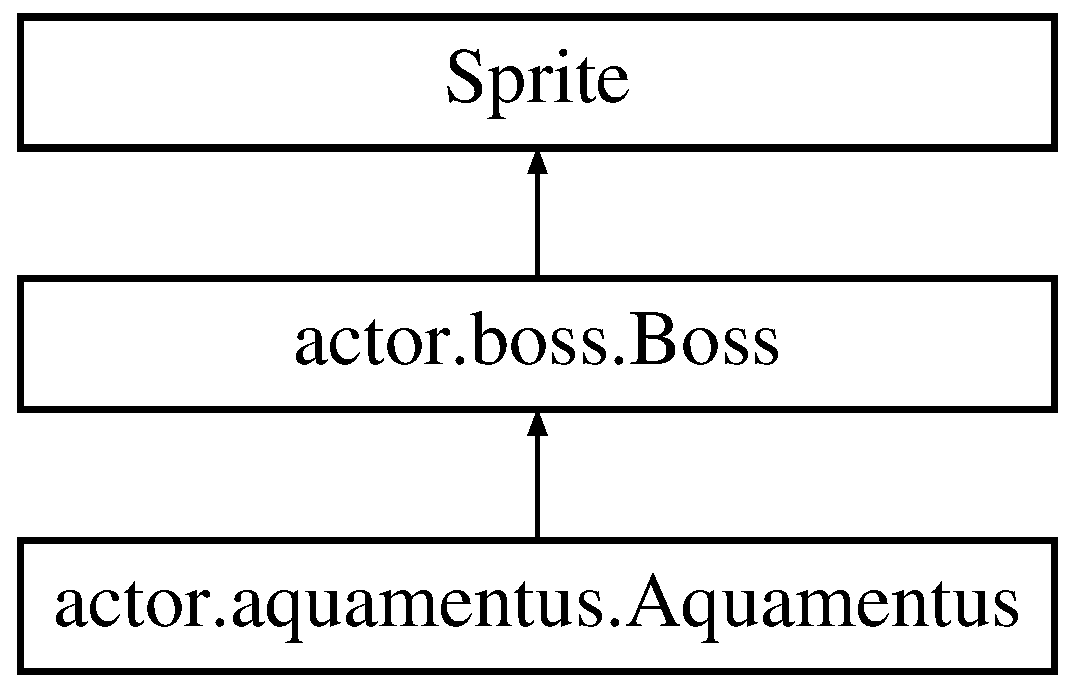
\includegraphics[height=3.000000cm]{classactor_1_1boss_1_1_boss}
\end{center}
\end{figure}
\subsection*{Public Member Functions}
\begin{DoxyCompactItemize}
\item 
def \hyperlink{classactor_1_1boss_1_1_boss_a8aff9faf12326306058968f2e6424420}{\+\_\+\+\_\+init\+\_\+\+\_\+} (self, x, y)
\begin{DoxyCompactList}\small\item\em Constructor for \hyperlink{classactor_1_1boss_1_1_boss}{Boss}. \end{DoxyCompactList}\item 
\mbox{\Hypertarget{classactor_1_1boss_1_1_boss_a5f510a5ea8387c4ccb1c5c36e54efa5d}\label{classactor_1_1boss_1_1_boss_a5f510a5ea8387c4ccb1c5c36e54efa5d}} 
def \hyperlink{classactor_1_1boss_1_1_boss_a5f510a5ea8387c4ccb1c5c36e54efa5d}{check\+State} (self)
\begin{DoxyCompactList}\small\item\em Empty function for evaluating \hyperlink{classactor_1_1boss_1_1_boss}{Boss} state. \end{DoxyCompactList}\item 
def \hyperlink{classactor_1_1boss_1_1_boss_aa4ec284ad22d7c18bfa7116e4b2863cf}{move} (self)
\begin{DoxyCompactList}\small\item\em Moves the \hyperlink{classactor_1_1boss_1_1_boss}{Boss}. \end{DoxyCompactList}\item 
\mbox{\Hypertarget{classactor_1_1boss_1_1_boss_a005977210760040c8af8f77972e068a0}\label{classactor_1_1boss_1_1_boss_a005977210760040c8af8f77972e068a0}} 
def \hyperlink{classactor_1_1boss_1_1_boss_a005977210760040c8af8f77972e068a0}{boss\+Logic} (self)
\begin{DoxyCompactList}\small\item\em Empty function for logic of \hyperlink{classactor_1_1boss_1_1_boss}{Boss}. \end{DoxyCompactList}\item 
def \hyperlink{classactor_1_1boss_1_1_boss_a0caeabbf20958679e55952559a2b74ee}{update} (self)
\begin{DoxyCompactList}\small\item\em Update loop for a \hyperlink{classactor_1_1boss_1_1_boss}{Boss}. \end{DoxyCompactList}\item 
def \hyperlink{classactor_1_1boss_1_1_boss_a6909e66b1a94f284ff34d2498a807c48}{hit} (self, dir)
\begin{DoxyCompactList}\small\item\em Hit dectetion for \hyperlink{classactor_1_1boss_1_1_boss}{Boss}. \end{DoxyCompactList}\end{DoxyCompactItemize}
\subsection*{Public Attributes}
\begin{DoxyCompactItemize}
\item 
\mbox{\Hypertarget{classactor_1_1boss_1_1_boss_a33e43928fc50f5c67693e2a224e2a67c}\label{classactor_1_1boss_1_1_boss_a33e43928fc50f5c67693e2a224e2a67c}} 
\hyperlink{classactor_1_1boss_1_1_boss_a33e43928fc50f5c67693e2a224e2a67c}{image}
\begin{DoxyCompactList}\small\item\em \hyperlink{classactor_1_1boss_1_1_boss}{Boss} Pygame surface. \end{DoxyCompactList}\item 
\mbox{\Hypertarget{classactor_1_1boss_1_1_boss_a0d5392b6ba783f8c3ad68221830f26ec}\label{classactor_1_1boss_1_1_boss_a0d5392b6ba783f8c3ad68221830f26ec}} 
\hyperlink{classactor_1_1boss_1_1_boss_a0d5392b6ba783f8c3ad68221830f26ec}{rect}
\begin{DoxyCompactList}\small\item\em Rectanlge that represents boss. \end{DoxyCompactList}\item 
\hyperlink{classactor_1_1boss_1_1_boss_a88b3aa7689b1d755e49e5dfbf7f30e86}{id}
\begin{DoxyCompactList}\small\item\em X postion of the boss. \end{DoxyCompactList}\item 
\mbox{\Hypertarget{classactor_1_1boss_1_1_boss_af197ba273deff12d755b58ba7d5dca8d}\label{classactor_1_1boss_1_1_boss_af197ba273deff12d755b58ba7d5dca8d}} 
\hyperlink{classactor_1_1boss_1_1_boss_af197ba273deff12d755b58ba7d5dca8d}{is\+Hit}
\begin{DoxyCompactList}\small\item\em Wether the boss is hit or not. \end{DoxyCompactList}\item 
\mbox{\Hypertarget{classactor_1_1boss_1_1_boss_a3bfec86c38534dee464d0f415812c90f}\label{classactor_1_1boss_1_1_boss_a3bfec86c38534dee464d0f415812c90f}} 
\hyperlink{classactor_1_1boss_1_1_boss_a3bfec86c38534dee464d0f415812c90f}{stuncount}
\begin{DoxyCompactList}\small\item\em The amount of stun frames the boss has remaining. \end{DoxyCompactList}\item 
\mbox{\Hypertarget{classactor_1_1boss_1_1_boss_a91aaf2376c5832f358df81e770d8e29f}\label{classactor_1_1boss_1_1_boss_a91aaf2376c5832f358df81e770d8e29f}} 
\hyperlink{classactor_1_1boss_1_1_boss_a91aaf2376c5832f358df81e770d8e29f}{max\+HP}
\begin{DoxyCompactList}\small\item\em \hyperlink{classactor_1_1boss_1_1_boss}{Boss}\textquotesingle{} max health. \end{DoxyCompactList}\item 
\mbox{\Hypertarget{classactor_1_1boss_1_1_boss_a86450ea10beac44c78eec4b05ddb09d0}\label{classactor_1_1boss_1_1_boss_a86450ea10beac44c78eec4b05ddb09d0}} 
\hyperlink{classactor_1_1boss_1_1_boss_a86450ea10beac44c78eec4b05ddb09d0}{HP}
\begin{DoxyCompactList}\small\item\em \hyperlink{classactor_1_1boss_1_1_boss}{Boss}\textquotesingle{} current health. \end{DoxyCompactList}\item 
\mbox{\Hypertarget{classactor_1_1boss_1_1_boss_a6a30d961adcdcf26fdcae6fb83801f8c}\label{classactor_1_1boss_1_1_boss_a6a30d961adcdcf26fdcae6fb83801f8c}} 
\hyperlink{classactor_1_1boss_1_1_boss_a6a30d961adcdcf26fdcae6fb83801f8c}{dmg}
\begin{DoxyCompactList}\small\item\em \hyperlink{classactor_1_1boss_1_1_boss}{Boss}\textquotesingle{} damage. \end{DoxyCompactList}\item 
\mbox{\Hypertarget{classactor_1_1boss_1_1_boss_a9884f8252599e809ccca0f09c13e7883}\label{classactor_1_1boss_1_1_boss_a9884f8252599e809ccca0f09c13e7883}} 
\hyperlink{classactor_1_1boss_1_1_boss_a9884f8252599e809ccca0f09c13e7883}{hit\+Count}
\begin{DoxyCompactList}\small\item\em \hyperlink{classactor_1_1boss_1_1_boss}{Boss}\textquotesingle{} hit count. \end{DoxyCompactList}\item 
\mbox{\Hypertarget{classactor_1_1boss_1_1_boss_aa8507ebe3d7bf619d0e630af700a18eb}\label{classactor_1_1boss_1_1_boss_aa8507ebe3d7bf619d0e630af700a18eb}} 
\hyperlink{classactor_1_1boss_1_1_boss_aa8507ebe3d7bf619d0e630af700a18eb}{x\+Speed}
\begin{DoxyCompactList}\small\item\em \hyperlink{classactor_1_1boss_1_1_boss}{Boss}\textquotesingle{} speed in the x direction. \end{DoxyCompactList}\item 
\mbox{\Hypertarget{classactor_1_1boss_1_1_boss_af3ffc8e8c2a5637f468355a055d4671f}\label{classactor_1_1boss_1_1_boss_af3ffc8e8c2a5637f468355a055d4671f}} 
\hyperlink{classactor_1_1boss_1_1_boss_af3ffc8e8c2a5637f468355a055d4671f}{y\+Speed}
\begin{DoxyCompactList}\small\item\em \hyperlink{classactor_1_1boss_1_1_boss}{Boss}\textquotesingle{} speed in the y direction. \end{DoxyCompactList}\item 
\mbox{\Hypertarget{classactor_1_1boss_1_1_boss_aca7d6c634a4af8380231efe3c2636080}\label{classactor_1_1boss_1_1_boss_aca7d6c634a4af8380231efe3c2636080}} 
\hyperlink{classactor_1_1boss_1_1_boss_aca7d6c634a4af8380231efe3c2636080}{frame\+Counter}
\begin{DoxyCompactList}\small\item\em Total number of frames the boss has been alive for. \end{DoxyCompactList}\end{DoxyCompactItemize}


\subsection{Detailed Description}
Superclass for representing a \hyperlink{classactor_1_1boss_1_1_boss}{Boss}. 

\subsection{Constructor \& Destructor Documentation}
\mbox{\Hypertarget{classactor_1_1boss_1_1_boss_a8aff9faf12326306058968f2e6424420}\label{classactor_1_1boss_1_1_boss_a8aff9faf12326306058968f2e6424420}} 
\index{actor\+::boss\+::\+Boss@{actor\+::boss\+::\+Boss}!\+\_\+\+\_\+init\+\_\+\+\_\+@{\+\_\+\+\_\+init\+\_\+\+\_\+}}
\index{\+\_\+\+\_\+init\+\_\+\+\_\+@{\+\_\+\+\_\+init\+\_\+\+\_\+}!actor\+::boss\+::\+Boss@{actor\+::boss\+::\+Boss}}
\subsubsection{\texorpdfstring{\+\_\+\+\_\+init\+\_\+\+\_\+()}{\_\_init\_\_()}}
{\footnotesize\ttfamily def actor.\+boss.\+Boss.\+\_\+\+\_\+init\+\_\+\+\_\+ (\begin{DoxyParamCaption}\item[{}]{self,  }\item[{}]{x,  }\item[{}]{y }\end{DoxyParamCaption})}



Constructor for \hyperlink{classactor_1_1boss_1_1_boss}{Boss}. 

Constructor takes two parameters, the x and y coordinates 
\begin{DoxyParams}{Parameters}
{\em x} & X coordinate of the starting postion of the \hyperlink{classactor_1_1boss_1_1_boss}{Boss} \\
\hline
{\em y} & Y coordinate of the starting postion of the \hyperlink{classactor_1_1boss_1_1_boss}{Boss} \\
\hline
\end{DoxyParams}


\subsection{Member Function Documentation}
\mbox{\Hypertarget{classactor_1_1boss_1_1_boss_a6909e66b1a94f284ff34d2498a807c48}\label{classactor_1_1boss_1_1_boss_a6909e66b1a94f284ff34d2498a807c48}} 
\index{actor\+::boss\+::\+Boss@{actor\+::boss\+::\+Boss}!hit@{hit}}
\index{hit@{hit}!actor\+::boss\+::\+Boss@{actor\+::boss\+::\+Boss}}
\subsubsection{\texorpdfstring{hit()}{hit()}}
{\footnotesize\ttfamily def actor.\+boss.\+Boss.\+hit (\begin{DoxyParamCaption}\item[{}]{self,  }\item[{}]{dir }\end{DoxyParamCaption})}



Hit dectetion for \hyperlink{classactor_1_1boss_1_1_boss}{Boss}. 

Handles health and iframes \mbox{\Hypertarget{classactor_1_1boss_1_1_boss_aa4ec284ad22d7c18bfa7116e4b2863cf}\label{classactor_1_1boss_1_1_boss_aa4ec284ad22d7c18bfa7116e4b2863cf}} 
\index{actor\+::boss\+::\+Boss@{actor\+::boss\+::\+Boss}!move@{move}}
\index{move@{move}!actor\+::boss\+::\+Boss@{actor\+::boss\+::\+Boss}}
\subsubsection{\texorpdfstring{move()}{move()}}
{\footnotesize\ttfamily def actor.\+boss.\+Boss.\+move (\begin{DoxyParamCaption}\item[{}]{self }\end{DoxyParamCaption})}



Moves the \hyperlink{classactor_1_1boss_1_1_boss}{Boss}. 

Adds the x speed and y speed to the x and y postion of the \hyperlink{classactor_1_1boss_1_1_boss}{Boss} \mbox{\Hypertarget{classactor_1_1boss_1_1_boss_a0caeabbf20958679e55952559a2b74ee}\label{classactor_1_1boss_1_1_boss_a0caeabbf20958679e55952559a2b74ee}} 
\index{actor\+::boss\+::\+Boss@{actor\+::boss\+::\+Boss}!update@{update}}
\index{update@{update}!actor\+::boss\+::\+Boss@{actor\+::boss\+::\+Boss}}
\subsubsection{\texorpdfstring{update()}{update()}}
{\footnotesize\ttfamily def actor.\+boss.\+Boss.\+update (\begin{DoxyParamCaption}\item[{}]{self }\end{DoxyParamCaption})}



Update loop for a \hyperlink{classactor_1_1boss_1_1_boss}{Boss}. 

Checks state, does the logic, and then moves \hyperlink{classactor_1_1boss_1_1_boss}{Boss} 

\subsection{Member Data Documentation}
\mbox{\Hypertarget{classactor_1_1boss_1_1_boss_a88b3aa7689b1d755e49e5dfbf7f30e86}\label{classactor_1_1boss_1_1_boss_a88b3aa7689b1d755e49e5dfbf7f30e86}} 
\index{actor\+::boss\+::\+Boss@{actor\+::boss\+::\+Boss}!id@{id}}
\index{id@{id}!actor\+::boss\+::\+Boss@{actor\+::boss\+::\+Boss}}
\subsubsection{\texorpdfstring{id}{id}}
{\footnotesize\ttfamily actor.\+boss.\+Boss.\+id}



X postion of the boss. 

Y postion of the boss \hyperlink{classactor_1_1boss_1_1_boss}{Boss} ID 

The documentation for this class was generated from the following file\+:\begin{DoxyCompactItemize}
\item 
src/actor/\hyperlink{boss_8py}{boss.\+py}\end{DoxyCompactItemize}

\hypertarget{classcollision_1_1door_1_1_door}{}\section{collision.\+door.\+Door Class Reference}
\label{classcollision_1_1door_1_1_door}\index{collision.\+door.\+Door@{collision.\+door.\+Door}}


Dungeon \hyperlink{classcollision_1_1door_1_1_door}{Door} Class  This class is used to place a door on one of four places of a dungeon room, to allow the player to walk through and traverse to other rooms within the dungeon.  


Inheritance diagram for collision.\+door.\+Door\+:\begin{figure}[H]
\begin{center}
\leavevmode
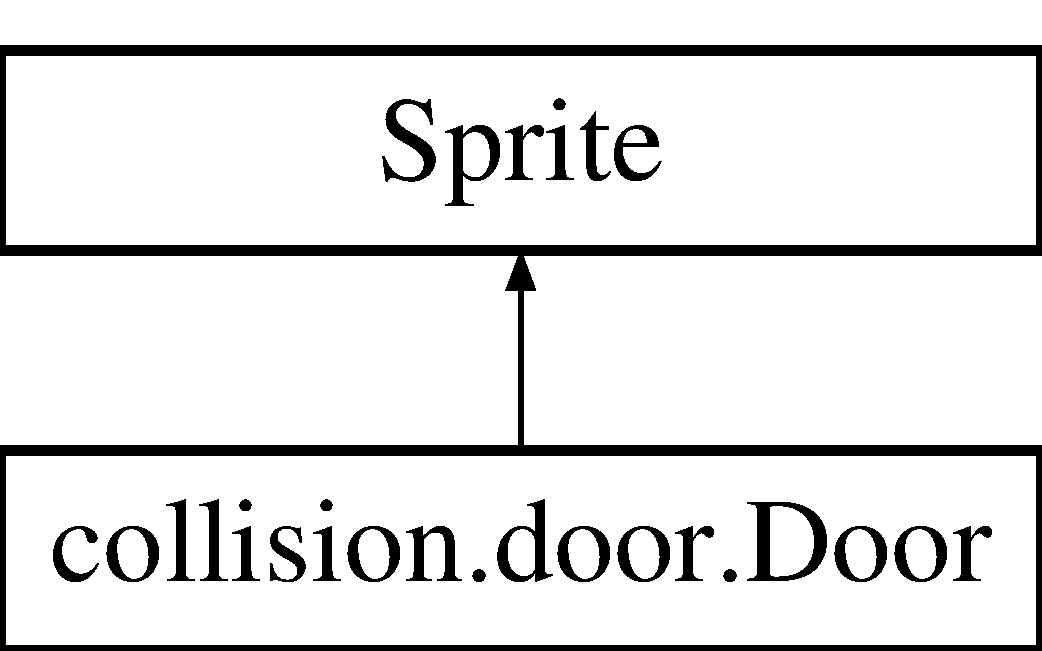
\includegraphics[height=2.000000cm]{classcollision_1_1door_1_1_door}
\end{center}
\end{figure}
\subsection*{Public Member Functions}
\begin{DoxyCompactItemize}
\item 
def \hyperlink{classcollision_1_1door_1_1_door_ab2b3e5e79d444388807a18f0c2022795}{\+\_\+\+\_\+init\+\_\+\+\_\+} (self, direction, \hyperlink{classcollision_1_1door_1_1_door_a22802ca389469576ecc1418e8c3e20b8}{state})
\begin{DoxyCompactList}\small\item\em \hyperlink{classcollision_1_1door_1_1_door}{Door} constructor, making a door on the specified side of the dungeon. \end{DoxyCompactList}\item 
def \hyperlink{classcollision_1_1door_1_1_door_a905d11890b7fa2fa789d67538136e685}{collision} (self, i)
\begin{DoxyCompactList}\small\item\em This method checks for collision with the \hyperlink{classcollision_1_1door_1_1_door}{Door} object and other sprite object. \end{DoxyCompactList}\item 
\mbox{\Hypertarget{classcollision_1_1door_1_1_door_a9ae0128993d925a4c6bcdb79936dbc4a}\label{classcollision_1_1door_1_1_door_a9ae0128993d925a4c6bcdb79936dbc4a}} 
def \hyperlink{classcollision_1_1door_1_1_door_a9ae0128993d925a4c6bcdb79936dbc4a}{open\+Door} (self)
\begin{DoxyCompactList}\small\item\em Function to set a door state and sprite to open  Changes a blocked door (state 1/2) to an open door (state 0), changing collision attributes and sprites respectively. \end{DoxyCompactList}\end{DoxyCompactItemize}
\subsection*{Public Attributes}
\begin{DoxyCompactItemize}
\item 
\mbox{\Hypertarget{classcollision_1_1door_1_1_door_a97c823f719c04f5bf8e5428e7b39b8b5}\label{classcollision_1_1door_1_1_door_a97c823f719c04f5bf8e5428e7b39b8b5}} 
{\bfseries dungeon\+\_\+sheet}
\item 
\hyperlink{classcollision_1_1door_1_1_door_a22802ca389469576ecc1418e8c3e20b8}{state}
\begin{DoxyCompactList}\small\item\em D\+O\+OR S\+T\+A\+TE 0 = open 1 = blocked (objective door) 2 = locked (key door) State of the door, integer value on whether the door is open(0), blocked by an objective(1), or locked(2) (blocked = eg. \end{DoxyCompactList}\item 
\mbox{\Hypertarget{classcollision_1_1door_1_1_door_a0ff4b9ac39898923fae449e1ed392b8a}\label{classcollision_1_1door_1_1_door_a0ff4b9ac39898923fae449e1ed392b8a}} 
{\bfseries dir}
\item 
\mbox{\Hypertarget{classcollision_1_1door_1_1_door_a4d8b68c958e4ec059f2e99e53e76abf1}\label{classcollision_1_1door_1_1_door_a4d8b68c958e4ec059f2e99e53e76abf1}} 
\hyperlink{classcollision_1_1door_1_1_door_a4d8b68c958e4ec059f2e99e53e76abf1}{image}
\begin{DoxyCompactList}\small\item\em Sprite image of the door. \end{DoxyCompactList}\item 
\mbox{\Hypertarget{classcollision_1_1door_1_1_door_a162269007487f8282278565e2f531a0c}\label{classcollision_1_1door_1_1_door_a162269007487f8282278565e2f531a0c}} 
\hyperlink{classcollision_1_1door_1_1_door_a162269007487f8282278565e2f531a0c}{rect}
\begin{DoxyCompactList}\small\item\em X and y coordinates of the image. \end{DoxyCompactList}\item 
\mbox{\Hypertarget{classcollision_1_1door_1_1_door_a101da4a463e317b8919c0bd1ad73b8df}\label{classcollision_1_1door_1_1_door_a101da4a463e317b8919c0bd1ad73b8df}} 
\hyperlink{classcollision_1_1door_1_1_door_a101da4a463e317b8919c0bd1ad73b8df}{id}
\begin{DoxyCompactList}\small\item\em Collision ID (to help other objects identify what they are colliding with and how to react) \end{DoxyCompactList}\end{DoxyCompactItemize}


\subsection{Detailed Description}
Dungeon \hyperlink{classcollision_1_1door_1_1_door}{Door} Class  This class is used to place a door on one of four places of a dungeon room, to allow the player to walk through and traverse to other rooms within the dungeon. 

\subsection{Constructor \& Destructor Documentation}
\mbox{\Hypertarget{classcollision_1_1door_1_1_door_ab2b3e5e79d444388807a18f0c2022795}\label{classcollision_1_1door_1_1_door_ab2b3e5e79d444388807a18f0c2022795}} 
\index{collision\+::door\+::\+Door@{collision\+::door\+::\+Door}!\+\_\+\+\_\+init\+\_\+\+\_\+@{\+\_\+\+\_\+init\+\_\+\+\_\+}}
\index{\+\_\+\+\_\+init\+\_\+\+\_\+@{\+\_\+\+\_\+init\+\_\+\+\_\+}!collision\+::door\+::\+Door@{collision\+::door\+::\+Door}}
\subsubsection{\texorpdfstring{\+\_\+\+\_\+init\+\_\+\+\_\+()}{\_\_init\_\_()}}
{\footnotesize\ttfamily def collision.\+door.\+Door.\+\_\+\+\_\+init\+\_\+\+\_\+ (\begin{DoxyParamCaption}\item[{}]{self,  }\item[{}]{direction,  }\item[{}]{state }\end{DoxyParamCaption})}



\hyperlink{classcollision_1_1door_1_1_door}{Door} constructor, making a door on the specified side of the dungeon. 


\begin{DoxyParams}{Parameters}
{\em direction} & Integer value of the wall the door will be on (direction from centre of room) \\
\hline
\end{DoxyParams}


\subsection{Member Function Documentation}
\mbox{\Hypertarget{classcollision_1_1door_1_1_door_a905d11890b7fa2fa789d67538136e685}\label{classcollision_1_1door_1_1_door_a905d11890b7fa2fa789d67538136e685}} 
\index{collision\+::door\+::\+Door@{collision\+::door\+::\+Door}!collision@{collision}}
\index{collision@{collision}!collision\+::door\+::\+Door@{collision\+::door\+::\+Door}}
\subsubsection{\texorpdfstring{collision()}{collision()}}
{\footnotesize\ttfamily def collision.\+door.\+Door.\+collision (\begin{DoxyParamCaption}\item[{}]{self,  }\item[{}]{i }\end{DoxyParamCaption})}



This method checks for collision with the \hyperlink{classcollision_1_1door_1_1_door}{Door} object and other sprite object. 

The collision will be checked with the \hyperlink{classcollision_1_1door_1_1_door}{Door} and other sprite object as the object collides with the wall. 
\begin{DoxyParams}{Parameters}
{\em i} & This is the sprite object that is passed into the method, and checks if the object is colliding with the \hyperlink{classcollision_1_1door_1_1_door}{Door} object, reseting the sprite objects location accordingly. \\
\hline
\end{DoxyParams}


\subsection{Member Data Documentation}
\mbox{\Hypertarget{classcollision_1_1door_1_1_door_a22802ca389469576ecc1418e8c3e20b8}\label{classcollision_1_1door_1_1_door_a22802ca389469576ecc1418e8c3e20b8}} 
\index{collision\+::door\+::\+Door@{collision\+::door\+::\+Door}!state@{state}}
\index{state@{state}!collision\+::door\+::\+Door@{collision\+::door\+::\+Door}}
\subsubsection{\texorpdfstring{state}{state}}
{\footnotesize\ttfamily collision.\+door.\+Door.\+state}



D\+O\+OR S\+T\+A\+TE 0 = open 1 = blocked (objective door) 2 = locked (key door) State of the door, integer value on whether the door is open(0), blocked by an objective(1), or locked(2) (blocked = eg. 

kill all enemies in room to open) 

The documentation for this class was generated from the following file\+:\begin{DoxyCompactItemize}
\item 
src/collision/\hyperlink{door_8py}{door.\+py}\end{DoxyCompactItemize}

\hypertarget{classactor_1_1enemy_1_1_enemy}{}\section{actor.\+enemy.\+Enemy Class Reference}
\label{classactor_1_1enemy_1_1_enemy}\index{actor.\+enemy.\+Enemy@{actor.\+enemy.\+Enemy}}


Superclass for representing an \hyperlink{classactor_1_1enemy_1_1_enemy}{Enemy}.  


Inheritance diagram for actor.\+enemy.\+Enemy\+:\begin{figure}[H]
\begin{center}
\leavevmode
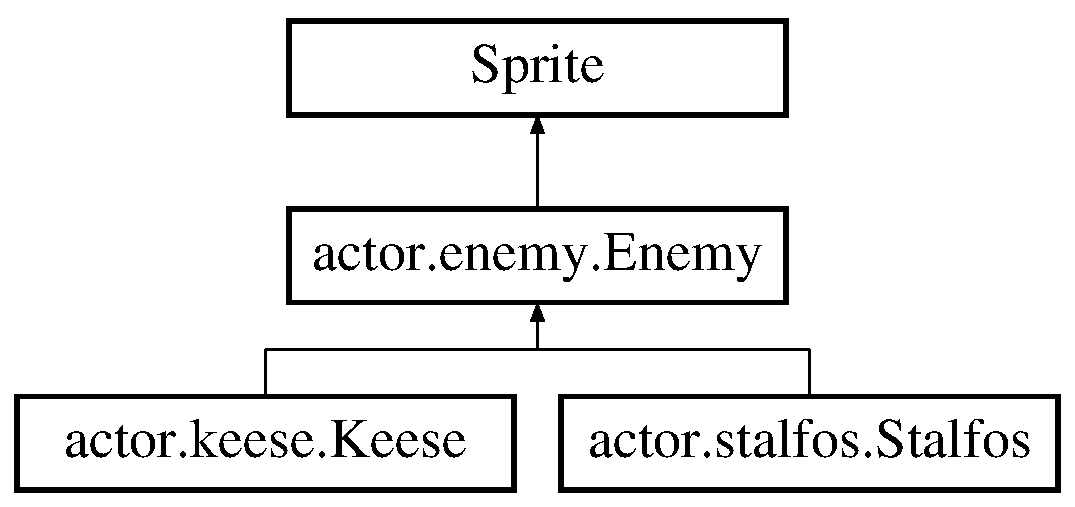
\includegraphics[height=3.000000cm]{classactor_1_1enemy_1_1_enemy}
\end{center}
\end{figure}
\subsection*{Public Member Functions}
\begin{DoxyCompactItemize}
\item 
def \hyperlink{classactor_1_1enemy_1_1_enemy_a6924d71617a5022d67fd46b36141dfd2}{\+\_\+\+\_\+init\+\_\+\+\_\+} (self, x, y)
\begin{DoxyCompactList}\small\item\em Constructor for \hyperlink{classactor_1_1enemy_1_1_enemy}{Enemy}. \end{DoxyCompactList}\item 
\mbox{\Hypertarget{classactor_1_1enemy_1_1_enemy_afa749d4d6a88fac474c3929ccd3b0753}\label{classactor_1_1enemy_1_1_enemy_afa749d4d6a88fac474c3929ccd3b0753}} 
def \hyperlink{classactor_1_1enemy_1_1_enemy_afa749d4d6a88fac474c3929ccd3b0753}{check\+State} (self)
\begin{DoxyCompactList}\small\item\em Empty function for evaluating \hyperlink{classactor_1_1enemy_1_1_enemy}{Enemy} state. \end{DoxyCompactList}\item 
def \hyperlink{classactor_1_1enemy_1_1_enemy_acae64f8e1e7e13ee7c440c74e3c214c8}{move} (self)
\begin{DoxyCompactList}\small\item\em Moves the \hyperlink{classactor_1_1enemy_1_1_enemy}{Enemy}. \end{DoxyCompactList}\item 
\mbox{\Hypertarget{classactor_1_1enemy_1_1_enemy_a94d38c945f048b873e33a539fb7cf502}\label{classactor_1_1enemy_1_1_enemy_a94d38c945f048b873e33a539fb7cf502}} 
def \hyperlink{classactor_1_1enemy_1_1_enemy_a94d38c945f048b873e33a539fb7cf502}{enemy\+Logic} (self)
\begin{DoxyCompactList}\small\item\em Empty function for logic of \hyperlink{classactor_1_1enemy_1_1_enemy}{Enemy}. \end{DoxyCompactList}\item 
def \hyperlink{classactor_1_1enemy_1_1_enemy_a5a7ad5761870721d959d491b33eb4908}{update} (self)
\begin{DoxyCompactList}\small\item\em Update loop for a \hyperlink{classactor_1_1enemy_1_1_enemy}{Enemy}. \end{DoxyCompactList}\item 
def \hyperlink{classactor_1_1enemy_1_1_enemy_a26b704148d13a372e1bf150937e30673}{hit} (self, direc)
\begin{DoxyCompactList}\small\item\em Hit dectetion for \hyperlink{classactor_1_1enemy_1_1_enemy}{Enemy}. \end{DoxyCompactList}\end{DoxyCompactItemize}
\subsection*{Public Attributes}
\begin{DoxyCompactItemize}
\item 
\mbox{\Hypertarget{classactor_1_1enemy_1_1_enemy_aa1cb2b099f1405c72c5aead1f72ca273}\label{classactor_1_1enemy_1_1_enemy_aa1cb2b099f1405c72c5aead1f72ca273}} 
\hyperlink{classactor_1_1enemy_1_1_enemy_aa1cb2b099f1405c72c5aead1f72ca273}{image}
\begin{DoxyCompactList}\small\item\em \hyperlink{classactor_1_1enemy_1_1_enemy}{Enemy} Pygame surface. \end{DoxyCompactList}\item 
\mbox{\Hypertarget{classactor_1_1enemy_1_1_enemy_aea251391a575a128f97cfd1806311f1e}\label{classactor_1_1enemy_1_1_enemy_aea251391a575a128f97cfd1806311f1e}} 
\hyperlink{classactor_1_1enemy_1_1_enemy_aea251391a575a128f97cfd1806311f1e}{rect}
\begin{DoxyCompactList}\small\item\em Rectanlge that represents enemy. \end{DoxyCompactList}\item 
\hyperlink{classactor_1_1enemy_1_1_enemy_a0e6ba00fdf6dd7aba8b872f7b21040a7}{id}
\begin{DoxyCompactList}\small\item\em \hyperlink{classactor_1_1enemy_1_1_enemy}{Enemy} x postion. \end{DoxyCompactList}\item 
\mbox{\Hypertarget{classactor_1_1enemy_1_1_enemy_ac706787533eed329ba4d3f69018dfd4f}\label{classactor_1_1enemy_1_1_enemy_ac706787533eed329ba4d3f69018dfd4f}} 
\hyperlink{classactor_1_1enemy_1_1_enemy_ac706787533eed329ba4d3f69018dfd4f}{is\+Hit}
\begin{DoxyCompactList}\small\item\em Wether the enemy is hit. \end{DoxyCompactList}\item 
\mbox{\Hypertarget{classactor_1_1enemy_1_1_enemy_a682e04fb5525441486f5ecfdd1a2d879}\label{classactor_1_1enemy_1_1_enemy_a682e04fb5525441486f5ecfdd1a2d879}} 
\hyperlink{classactor_1_1enemy_1_1_enemy_a682e04fb5525441486f5ecfdd1a2d879}{stuncount}
\begin{DoxyCompactList}\small\item\em Remaining stun frames. \end{DoxyCompactList}\item 
\mbox{\Hypertarget{classactor_1_1enemy_1_1_enemy_ad57e864feaa058d6e05344a5131e3c3b}\label{classactor_1_1enemy_1_1_enemy_ad57e864feaa058d6e05344a5131e3c3b}} 
\hyperlink{classactor_1_1enemy_1_1_enemy_ad57e864feaa058d6e05344a5131e3c3b}{max\+HP}
\begin{DoxyCompactList}\small\item\em \hyperlink{classactor_1_1enemy_1_1_enemy}{Enemy} max health. \end{DoxyCompactList}\item 
\mbox{\Hypertarget{classactor_1_1enemy_1_1_enemy_a628179612c6af830270a9fd49e147bce}\label{classactor_1_1enemy_1_1_enemy_a628179612c6af830270a9fd49e147bce}} 
\hyperlink{classactor_1_1enemy_1_1_enemy_a628179612c6af830270a9fd49e147bce}{HP}
\begin{DoxyCompactList}\small\item\em \hyperlink{classactor_1_1enemy_1_1_enemy}{Enemy} current health. \end{DoxyCompactList}\item 
\mbox{\Hypertarget{classactor_1_1enemy_1_1_enemy_a23382d6dec9cbf34c1feec91de95db36}\label{classactor_1_1enemy_1_1_enemy_a23382d6dec9cbf34c1feec91de95db36}} 
\hyperlink{classactor_1_1enemy_1_1_enemy_a23382d6dec9cbf34c1feec91de95db36}{dmg}
\begin{DoxyCompactList}\small\item\em \hyperlink{classactor_1_1enemy_1_1_enemy}{Enemy} damage. \end{DoxyCompactList}\item 
\hyperlink{classactor_1_1enemy_1_1_enemy_aaa23681089031060de8abdf44956b7d1}{hit\+Count}
\begin{DoxyCompactList}\small\item\em This represents the buffer for the number of hits for the \hyperlink{classactor_1_1enemy_1_1_enemy}{Enemy} after being hit by player character. \end{DoxyCompactList}\item 
\hyperlink{classactor_1_1enemy_1_1_enemy_acc0b053f7922d48e2b76b2a0341c2c0c}{hitdir}
\begin{DoxyCompactList}\small\item\em Represents the direction \hyperlink{classactor_1_1enemy_1_1_enemy}{Enemy} is hit in by player character attack. \end{DoxyCompactList}\item 
\mbox{\Hypertarget{classactor_1_1enemy_1_1_enemy_aeb8e66f955c0233222186a0b31ffebec}\label{classactor_1_1enemy_1_1_enemy_aeb8e66f955c0233222186a0b31ffebec}} 
\hyperlink{classactor_1_1enemy_1_1_enemy_aeb8e66f955c0233222186a0b31ffebec}{x\+Speed}
\begin{DoxyCompactList}\small\item\em \hyperlink{classactor_1_1enemy_1_1_enemy}{Enemy} speed in the x direction. \end{DoxyCompactList}\item 
\mbox{\Hypertarget{classactor_1_1enemy_1_1_enemy_a9df94b7c1824222274977377fc61de0b}\label{classactor_1_1enemy_1_1_enemy_a9df94b7c1824222274977377fc61de0b}} 
\hyperlink{classactor_1_1enemy_1_1_enemy_a9df94b7c1824222274977377fc61de0b}{y\+Speed}
\begin{DoxyCompactList}\small\item\em \hyperlink{classactor_1_1enemy_1_1_enemy}{Enemy} speed in the y direction. \end{DoxyCompactList}\item 
\mbox{\Hypertarget{classactor_1_1enemy_1_1_enemy_a2c89ef588742abcdeb22215bb381d69b}\label{classactor_1_1enemy_1_1_enemy_a2c89ef588742abcdeb22215bb381d69b}} 
\hyperlink{classactor_1_1enemy_1_1_enemy_a2c89ef588742abcdeb22215bb381d69b}{frame\+Counter}
\begin{DoxyCompactList}\small\item\em Total number of frames the enemy has been alive. \end{DoxyCompactList}\end{DoxyCompactItemize}


\subsection{Detailed Description}
Superclass for representing an \hyperlink{classactor_1_1enemy_1_1_enemy}{Enemy}. 

\subsection{Constructor \& Destructor Documentation}
\mbox{\Hypertarget{classactor_1_1enemy_1_1_enemy_a6924d71617a5022d67fd46b36141dfd2}\label{classactor_1_1enemy_1_1_enemy_a6924d71617a5022d67fd46b36141dfd2}} 
\index{actor\+::enemy\+::\+Enemy@{actor\+::enemy\+::\+Enemy}!\+\_\+\+\_\+init\+\_\+\+\_\+@{\+\_\+\+\_\+init\+\_\+\+\_\+}}
\index{\+\_\+\+\_\+init\+\_\+\+\_\+@{\+\_\+\+\_\+init\+\_\+\+\_\+}!actor\+::enemy\+::\+Enemy@{actor\+::enemy\+::\+Enemy}}
\subsubsection{\texorpdfstring{\+\_\+\+\_\+init\+\_\+\+\_\+()}{\_\_init\_\_()}}
{\footnotesize\ttfamily def actor.\+enemy.\+Enemy.\+\_\+\+\_\+init\+\_\+\+\_\+ (\begin{DoxyParamCaption}\item[{}]{self,  }\item[{}]{x,  }\item[{}]{y }\end{DoxyParamCaption})}



Constructor for \hyperlink{classactor_1_1enemy_1_1_enemy}{Enemy}. 

Constructor takes two parameters, the x and y coordinates 
\begin{DoxyParams}{Parameters}
{\em x} & X coordinate of the starting postion of the \hyperlink{classactor_1_1enemy_1_1_enemy}{Enemy} \\
\hline
{\em y} & Y coordinate of the starting postion of the \hyperlink{classactor_1_1enemy_1_1_enemy}{Enemy} \\
\hline
\end{DoxyParams}


\subsection{Member Function Documentation}
\mbox{\Hypertarget{classactor_1_1enemy_1_1_enemy_a26b704148d13a372e1bf150937e30673}\label{classactor_1_1enemy_1_1_enemy_a26b704148d13a372e1bf150937e30673}} 
\index{actor\+::enemy\+::\+Enemy@{actor\+::enemy\+::\+Enemy}!hit@{hit}}
\index{hit@{hit}!actor\+::enemy\+::\+Enemy@{actor\+::enemy\+::\+Enemy}}
\subsubsection{\texorpdfstring{hit()}{hit()}}
{\footnotesize\ttfamily def actor.\+enemy.\+Enemy.\+hit (\begin{DoxyParamCaption}\item[{}]{self,  }\item[{}]{direc }\end{DoxyParamCaption})}



Hit dectetion for \hyperlink{classactor_1_1enemy_1_1_enemy}{Enemy}. 

Handles health, iframes and knockback direction 
\begin{DoxyParams}{Parameters}
{\em direc} & Direction of the knockback \\
\hline
\end{DoxyParams}
\mbox{\Hypertarget{classactor_1_1enemy_1_1_enemy_acae64f8e1e7e13ee7c440c74e3c214c8}\label{classactor_1_1enemy_1_1_enemy_acae64f8e1e7e13ee7c440c74e3c214c8}} 
\index{actor\+::enemy\+::\+Enemy@{actor\+::enemy\+::\+Enemy}!move@{move}}
\index{move@{move}!actor\+::enemy\+::\+Enemy@{actor\+::enemy\+::\+Enemy}}
\subsubsection{\texorpdfstring{move()}{move()}}
{\footnotesize\ttfamily def actor.\+enemy.\+Enemy.\+move (\begin{DoxyParamCaption}\item[{}]{self }\end{DoxyParamCaption})}



Moves the \hyperlink{classactor_1_1enemy_1_1_enemy}{Enemy}. 

Adds the x speed and y speed to the x and y postion of the \hyperlink{classactor_1_1enemy_1_1_enemy}{Enemy} \mbox{\Hypertarget{classactor_1_1enemy_1_1_enemy_a5a7ad5761870721d959d491b33eb4908}\label{classactor_1_1enemy_1_1_enemy_a5a7ad5761870721d959d491b33eb4908}} 
\index{actor\+::enemy\+::\+Enemy@{actor\+::enemy\+::\+Enemy}!update@{update}}
\index{update@{update}!actor\+::enemy\+::\+Enemy@{actor\+::enemy\+::\+Enemy}}
\subsubsection{\texorpdfstring{update()}{update()}}
{\footnotesize\ttfamily def actor.\+enemy.\+Enemy.\+update (\begin{DoxyParamCaption}\item[{}]{self }\end{DoxyParamCaption})}



Update loop for a \hyperlink{classactor_1_1enemy_1_1_enemy}{Enemy}. 

Checks state, does the logic, and then moves \hyperlink{classactor_1_1enemy_1_1_enemy}{Enemy} 

\subsection{Member Data Documentation}
\mbox{\Hypertarget{classactor_1_1enemy_1_1_enemy_aaa23681089031060de8abdf44956b7d1}\label{classactor_1_1enemy_1_1_enemy_aaa23681089031060de8abdf44956b7d1}} 
\index{actor\+::enemy\+::\+Enemy@{actor\+::enemy\+::\+Enemy}!hit\+Count@{hit\+Count}}
\index{hit\+Count@{hit\+Count}!actor\+::enemy\+::\+Enemy@{actor\+::enemy\+::\+Enemy}}
\subsubsection{\texorpdfstring{hit\+Count}{hitCount}}
{\footnotesize\ttfamily actor.\+enemy.\+Enemy.\+hit\+Count}



This represents the buffer for the number of hits for the \hyperlink{classactor_1_1enemy_1_1_enemy}{Enemy} after being hit by player character. 

\mbox{\Hypertarget{classactor_1_1enemy_1_1_enemy_acc0b053f7922d48e2b76b2a0341c2c0c}\label{classactor_1_1enemy_1_1_enemy_acc0b053f7922d48e2b76b2a0341c2c0c}} 
\index{actor\+::enemy\+::\+Enemy@{actor\+::enemy\+::\+Enemy}!hitdir@{hitdir}}
\index{hitdir@{hitdir}!actor\+::enemy\+::\+Enemy@{actor\+::enemy\+::\+Enemy}}
\subsubsection{\texorpdfstring{hitdir}{hitdir}}
{\footnotesize\ttfamily actor.\+enemy.\+Enemy.\+hitdir}



Represents the direction \hyperlink{classactor_1_1enemy_1_1_enemy}{Enemy} is hit in by player character attack. 

\mbox{\Hypertarget{classactor_1_1enemy_1_1_enemy_a0e6ba00fdf6dd7aba8b872f7b21040a7}\label{classactor_1_1enemy_1_1_enemy_a0e6ba00fdf6dd7aba8b872f7b21040a7}} 
\index{actor\+::enemy\+::\+Enemy@{actor\+::enemy\+::\+Enemy}!id@{id}}
\index{id@{id}!actor\+::enemy\+::\+Enemy@{actor\+::enemy\+::\+Enemy}}
\subsubsection{\texorpdfstring{id}{id}}
{\footnotesize\ttfamily actor.\+enemy.\+Enemy.\+id}



\hyperlink{classactor_1_1enemy_1_1_enemy}{Enemy} x postion. 

\hyperlink{classactor_1_1enemy_1_1_enemy}{Enemy} y postion \hyperlink{classactor_1_1enemy_1_1_enemy}{Enemy} Id type 

The documentation for this class was generated from the following file\+:\begin{DoxyCompactItemize}
\item 
src/actor/\hyperlink{enemy_8py}{enemy.\+py}\end{DoxyCompactItemize}

\hypertarget{classactor_1_1fireball_1_1_fireball}{}\section{actor.\+fireball.\+Fireball Class Reference}
\label{classactor_1_1fireball_1_1_fireball}\index{actor.\+fireball.\+Fireball@{actor.\+fireball.\+Fireball}}


This class represents the \hyperlink{classactor_1_1fireball_1_1_fireball}{Fireball} object.  


Inheritance diagram for actor.\+fireball.\+Fireball\+:\begin{figure}[H]
\begin{center}
\leavevmode
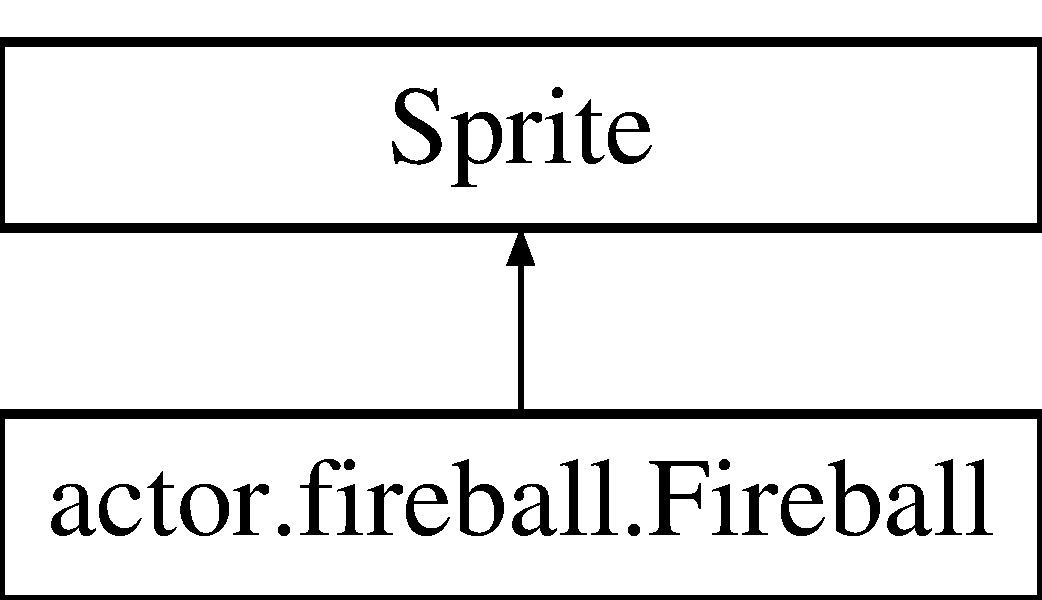
\includegraphics[height=2.000000cm]{classactor_1_1fireball_1_1_fireball}
\end{center}
\end{figure}
\subsection*{Public Member Functions}
\begin{DoxyCompactItemize}
\item 
def \hyperlink{classactor_1_1fireball_1_1_fireball_a8e8de406c4754cea725b3800053bbabc}{\+\_\+\+\_\+init\+\_\+\+\_\+} (self, x, y, \hyperlink{classactor_1_1fireball_1_1_fireball_a6708bc69526dffd73c714657dbfa0625}{x\+Speed}, \hyperlink{classactor_1_1fireball_1_1_fireball_a87f95efd62b2ebc27b5f742d9ae50ca6}{y\+Speed})
\begin{DoxyCompactList}\small\item\em Constructor for \hyperlink{classactor_1_1fireball_1_1_fireball}{Fireball}. \end{DoxyCompactList}\item 
def \hyperlink{classactor_1_1fireball_1_1_fireball_a5a93196e521c8cca75aac1dc7f9080a4}{start} (self, x, y, xs, ys)
\begin{DoxyCompactList}\small\item\em Starts the \hyperlink{classactor_1_1fireball_1_1_fireball}{Fireball}\textquotesingle{}s movement. \end{DoxyCompactList}\item 
def \hyperlink{classactor_1_1fireball_1_1_fireball_ab4e6a41b951134c42579f056ab0b4d43}{end} (self)
\begin{DoxyCompactList}\small\item\em Ends the \hyperlink{classactor_1_1fireball_1_1_fireball}{Fireball}\textquotesingle{}s movement. \end{DoxyCompactList}\item 
def \hyperlink{classactor_1_1fireball_1_1_fireball_a21e2ae2502f54f7a247f9201c167bc5e}{hit} (self, dir)
\begin{DoxyCompactList}\small\item\em Empty function for being hit by player. \end{DoxyCompactList}\item 
def \hyperlink{classactor_1_1fireball_1_1_fireball_abf7cee468c753aa1ed23bd45cd7a7bdc}{check\+State} (self)
\begin{DoxyCompactList}\small\item\em Evaluates the state of the \hyperlink{classactor_1_1fireball_1_1_fireball}{Fireball}. \end{DoxyCompactList}\item 
def \hyperlink{classactor_1_1fireball_1_1_fireball_a7eca2eb84a6f46f23df4a092edd044ac}{move} (self)
\begin{DoxyCompactList}\small\item\em Moves the \hyperlink{classactor_1_1fireball_1_1_fireball}{Fireball}. \end{DoxyCompactList}\item 
def \hyperlink{classactor_1_1fireball_1_1_fireball_ad19f7a375bf095055aadce16138d5713}{logic} (self)
\begin{DoxyCompactList}\small\item\em Updates the \hyperlink{classactor_1_1fireball_1_1_fireball}{Fireball} sprite. \end{DoxyCompactList}\item 
def \hyperlink{classactor_1_1fireball_1_1_fireball_af65dbfd4e9993637a797cc9cf7475238}{update} (self)
\begin{DoxyCompactList}\small\item\em Updates the \hyperlink{classactor_1_1fireball_1_1_fireball}{Fireball} every frame \end{DoxyCompactList}\end{DoxyCompactItemize}
\subsection*{Public Attributes}
\begin{DoxyCompactItemize}
\item 
\hyperlink{classactor_1_1fireball_1_1_fireball_a5dbeecf7c79f7dd02bd262048b79f908}{image}
\begin{DoxyCompactList}\small\item\em \hyperlink{classactor_1_1fireball_1_1_fireball}{Fireball} surface. \end{DoxyCompactList}\item 
\mbox{\Hypertarget{classactor_1_1fireball_1_1_fireball_a23e0fa743f75f08f14448d2ab61782e0}\label{classactor_1_1fireball_1_1_fireball_a23e0fa743f75f08f14448d2ab61782e0}} 
\hyperlink{classactor_1_1fireball_1_1_fireball_a23e0fa743f75f08f14448d2ab61782e0}{rect}
\begin{DoxyCompactList}\small\item\em Rectangle that represents the fireball. \end{DoxyCompactList}\item 
\hyperlink{classactor_1_1fireball_1_1_fireball_aeb50a9203c4b4a9d66934feadb95d8c0}{id}
\begin{DoxyCompactList}\small\item\em \hyperlink{classactor_1_1fireball_1_1_fireball}{Fireball} x postion. \end{DoxyCompactList}\item 
\mbox{\Hypertarget{classactor_1_1fireball_1_1_fireball_a5bb7cb975378011380c177af107bd50f}\label{classactor_1_1fireball_1_1_fireball_a5bb7cb975378011380c177af107bd50f}} 
\hyperlink{classactor_1_1fireball_1_1_fireball_a5bb7cb975378011380c177af107bd50f}{is\+Hit}
\begin{DoxyCompactList}\small\item\em Wether the fireball is hit. \end{DoxyCompactList}\item 
\mbox{\Hypertarget{classactor_1_1fireball_1_1_fireball_a6210caf7f7eb813b6a2f1b868670af94}\label{classactor_1_1fireball_1_1_fireball_a6210caf7f7eb813b6a2f1b868670af94}} 
\hyperlink{classactor_1_1fireball_1_1_fireball_a6210caf7f7eb813b6a2f1b868670af94}{dmg}
\begin{DoxyCompactList}\small\item\em \hyperlink{classactor_1_1fireball_1_1_fireball}{Fireball} damage. \end{DoxyCompactList}\item 
\mbox{\Hypertarget{classactor_1_1fireball_1_1_fireball_a28bb6b364aba11762bbb763ebb5c4e72}\label{classactor_1_1fireball_1_1_fireball_a28bb6b364aba11762bbb763ebb5c4e72}} 
\hyperlink{classactor_1_1fireball_1_1_fireball_a28bb6b364aba11762bbb763ebb5c4e72}{hit\+Count}
\begin{DoxyCompactList}\small\item\em \hyperlink{classactor_1_1fireball_1_1_fireball}{Fireball} hit frames. \end{DoxyCompactList}\item 
\mbox{\Hypertarget{classactor_1_1fireball_1_1_fireball_a6708bc69526dffd73c714657dbfa0625}\label{classactor_1_1fireball_1_1_fireball_a6708bc69526dffd73c714657dbfa0625}} 
\hyperlink{classactor_1_1fireball_1_1_fireball_a6708bc69526dffd73c714657dbfa0625}{x\+Speed}
\begin{DoxyCompactList}\small\item\em \hyperlink{classactor_1_1fireball_1_1_fireball}{Fireball} speed in the x direction. \end{DoxyCompactList}\item 
\mbox{\Hypertarget{classactor_1_1fireball_1_1_fireball_a87f95efd62b2ebc27b5f742d9ae50ca6}\label{classactor_1_1fireball_1_1_fireball_a87f95efd62b2ebc27b5f742d9ae50ca6}} 
\hyperlink{classactor_1_1fireball_1_1_fireball_a87f95efd62b2ebc27b5f742d9ae50ca6}{y\+Speed}
\begin{DoxyCompactList}\small\item\em \hyperlink{classactor_1_1fireball_1_1_fireball}{Fireball} speed in the y direction. \end{DoxyCompactList}\item 
\mbox{\Hypertarget{classactor_1_1fireball_1_1_fireball_a6569e0533d043a88a4e0d3393ac36c40}\label{classactor_1_1fireball_1_1_fireball_a6569e0533d043a88a4e0d3393ac36c40}} 
\hyperlink{classactor_1_1fireball_1_1_fireball_a6569e0533d043a88a4e0d3393ac36c40}{frame\+Counter}
\begin{DoxyCompactList}\small\item\em Total number of frames fireball is alive. \end{DoxyCompactList}\item 
\mbox{\Hypertarget{classactor_1_1fireball_1_1_fireball_aa034598272954824e2e9c2aac4c1a34d}\label{classactor_1_1fireball_1_1_fireball_aa034598272954824e2e9c2aac4c1a34d}} 
{\bfseries sprites}
\item 
\mbox{\Hypertarget{classactor_1_1fireball_1_1_fireball_a2e9d4868a5b6a944121481b9f82bd37d}\label{classactor_1_1fireball_1_1_fireball_a2e9d4868a5b6a944121481b9f82bd37d}} 
\hyperlink{classactor_1_1fireball_1_1_fireball_a2e9d4868a5b6a944121481b9f82bd37d}{obj}
\begin{DoxyCompactList}\small\item\em \hyperlink{classactor_1_1fireball_1_1_fireball}{Fireball} collision list. \end{DoxyCompactList}\item 
\mbox{\Hypertarget{classactor_1_1fireball_1_1_fireball_a73fd4922f27fe97472bd1e66ec809077}\label{classactor_1_1fireball_1_1_fireball_a73fd4922f27fe97472bd1e66ec809077}} 
\hyperlink{classactor_1_1fireball_1_1_fireball_a73fd4922f27fe97472bd1e66ec809077}{sprite\+Index}
\begin{DoxyCompactList}\small\item\em Sprite list index. \end{DoxyCompactList}\end{DoxyCompactItemize}


\subsection{Detailed Description}
This class represents the \hyperlink{classactor_1_1fireball_1_1_fireball}{Fireball} object. 

\subsection{Constructor \& Destructor Documentation}
\mbox{\Hypertarget{classactor_1_1fireball_1_1_fireball_a8e8de406c4754cea725b3800053bbabc}\label{classactor_1_1fireball_1_1_fireball_a8e8de406c4754cea725b3800053bbabc}} 
\index{actor\+::fireball\+::\+Fireball@{actor\+::fireball\+::\+Fireball}!\+\_\+\+\_\+init\+\_\+\+\_\+@{\+\_\+\+\_\+init\+\_\+\+\_\+}}
\index{\+\_\+\+\_\+init\+\_\+\+\_\+@{\+\_\+\+\_\+init\+\_\+\+\_\+}!actor\+::fireball\+::\+Fireball@{actor\+::fireball\+::\+Fireball}}
\subsubsection{\texorpdfstring{\+\_\+\+\_\+init\+\_\+\+\_\+()}{\_\_init\_\_()}}
{\footnotesize\ttfamily def actor.\+fireball.\+Fireball.\+\_\+\+\_\+init\+\_\+\+\_\+ (\begin{DoxyParamCaption}\item[{}]{self,  }\item[{}]{x,  }\item[{}]{y,  }\item[{}]{x\+Speed,  }\item[{}]{y\+Speed }\end{DoxyParamCaption})}



Constructor for \hyperlink{classactor_1_1fireball_1_1_fireball}{Fireball}. 

Constructor takes four parameters, the x and y coordinates and the x and y speeds 
\begin{DoxyParams}{Parameters}
{\em x} & X coordinate of the starting postion of the \hyperlink{classactor_1_1fireball_1_1_fireball}{Fireball} \\
\hline
{\em y} & Y coordinate of the starting postion of the \hyperlink{classactor_1_1fireball_1_1_fireball}{Fireball} \\
\hline
{\em x\+Speed} & The speed in the x direction of the \hyperlink{classactor_1_1fireball_1_1_fireball}{Fireball} \\
\hline
{\em y\+Speed} & The speed in the y direction of the \hyperlink{classactor_1_1fireball_1_1_fireball}{Fireball} \\
\hline
\end{DoxyParams}


\subsection{Member Function Documentation}
\mbox{\Hypertarget{classactor_1_1fireball_1_1_fireball_abf7cee468c753aa1ed23bd45cd7a7bdc}\label{classactor_1_1fireball_1_1_fireball_abf7cee468c753aa1ed23bd45cd7a7bdc}} 
\index{actor\+::fireball\+::\+Fireball@{actor\+::fireball\+::\+Fireball}!check\+State@{check\+State}}
\index{check\+State@{check\+State}!actor\+::fireball\+::\+Fireball@{actor\+::fireball\+::\+Fireball}}
\subsubsection{\texorpdfstring{check\+State()}{checkState()}}
{\footnotesize\ttfamily def actor.\+fireball.\+Fireball.\+check\+State (\begin{DoxyParamCaption}\item[{}]{self }\end{DoxyParamCaption})}



Evaluates the state of the \hyperlink{classactor_1_1fireball_1_1_fireball}{Fireball}. 

Checks for collision with walls, doors, and players \mbox{\Hypertarget{classactor_1_1fireball_1_1_fireball_ab4e6a41b951134c42579f056ab0b4d43}\label{classactor_1_1fireball_1_1_fireball_ab4e6a41b951134c42579f056ab0b4d43}} 
\index{actor\+::fireball\+::\+Fireball@{actor\+::fireball\+::\+Fireball}!end@{end}}
\index{end@{end}!actor\+::fireball\+::\+Fireball@{actor\+::fireball\+::\+Fireball}}
\subsubsection{\texorpdfstring{end()}{end()}}
{\footnotesize\ttfamily def actor.\+fireball.\+Fireball.\+end (\begin{DoxyParamCaption}\item[{}]{self }\end{DoxyParamCaption})}



Ends the \hyperlink{classactor_1_1fireball_1_1_fireball}{Fireball}\textquotesingle{}s movement. 

Sets the x and y speed to 0 and places the \hyperlink{classactor_1_1fireball_1_1_fireball}{Fireball} of screen \mbox{\Hypertarget{classactor_1_1fireball_1_1_fireball_a21e2ae2502f54f7a247f9201c167bc5e}\label{classactor_1_1fireball_1_1_fireball_a21e2ae2502f54f7a247f9201c167bc5e}} 
\index{actor\+::fireball\+::\+Fireball@{actor\+::fireball\+::\+Fireball}!hit@{hit}}
\index{hit@{hit}!actor\+::fireball\+::\+Fireball@{actor\+::fireball\+::\+Fireball}}
\subsubsection{\texorpdfstring{hit()}{hit()}}
{\footnotesize\ttfamily def actor.\+fireball.\+Fireball.\+hit (\begin{DoxyParamCaption}\item[{}]{self,  }\item[{}]{dir }\end{DoxyParamCaption})}



Empty function for being hit by player. 

Needs to exist for when player sword collides with \hyperlink{classactor_1_1fireball_1_1_fireball}{Fireball} \mbox{\Hypertarget{classactor_1_1fireball_1_1_fireball_ad19f7a375bf095055aadce16138d5713}\label{classactor_1_1fireball_1_1_fireball_ad19f7a375bf095055aadce16138d5713}} 
\index{actor\+::fireball\+::\+Fireball@{actor\+::fireball\+::\+Fireball}!logic@{logic}}
\index{logic@{logic}!actor\+::fireball\+::\+Fireball@{actor\+::fireball\+::\+Fireball}}
\subsubsection{\texorpdfstring{logic()}{logic()}}
{\footnotesize\ttfamily def actor.\+fireball.\+Fireball.\+logic (\begin{DoxyParamCaption}\item[{}]{self }\end{DoxyParamCaption})}



Updates the \hyperlink{classactor_1_1fireball_1_1_fireball}{Fireball} sprite. 

Swaps between the 2 sprites every 15 frames \mbox{\Hypertarget{classactor_1_1fireball_1_1_fireball_a7eca2eb84a6f46f23df4a092edd044ac}\label{classactor_1_1fireball_1_1_fireball_a7eca2eb84a6f46f23df4a092edd044ac}} 
\index{actor\+::fireball\+::\+Fireball@{actor\+::fireball\+::\+Fireball}!move@{move}}
\index{move@{move}!actor\+::fireball\+::\+Fireball@{actor\+::fireball\+::\+Fireball}}
\subsubsection{\texorpdfstring{move()}{move()}}
{\footnotesize\ttfamily def actor.\+fireball.\+Fireball.\+move (\begin{DoxyParamCaption}\item[{}]{self }\end{DoxyParamCaption})}



Moves the \hyperlink{classactor_1_1fireball_1_1_fireball}{Fireball}. 

Adds the x speed and y speed to the x and y postion of the \hyperlink{classactor_1_1fireball_1_1_fireball}{Fireball} \mbox{\Hypertarget{classactor_1_1fireball_1_1_fireball_a5a93196e521c8cca75aac1dc7f9080a4}\label{classactor_1_1fireball_1_1_fireball_a5a93196e521c8cca75aac1dc7f9080a4}} 
\index{actor\+::fireball\+::\+Fireball@{actor\+::fireball\+::\+Fireball}!start@{start}}
\index{start@{start}!actor\+::fireball\+::\+Fireball@{actor\+::fireball\+::\+Fireball}}
\subsubsection{\texorpdfstring{start()}{start()}}
{\footnotesize\ttfamily def actor.\+fireball.\+Fireball.\+start (\begin{DoxyParamCaption}\item[{}]{self,  }\item[{}]{x,  }\item[{}]{y,  }\item[{}]{xs,  }\item[{}]{ys }\end{DoxyParamCaption})}



Starts the \hyperlink{classactor_1_1fireball_1_1_fireball}{Fireball}\textquotesingle{}s movement. 

Sets the x and y postions and x and y speeds for \hyperlink{classactor_1_1fireball_1_1_fireball}{Fireball} 
\begin{DoxyParams}{Parameters}
{\em x} & X coordinate of where the \hyperlink{classactor_1_1fireball_1_1_fireball}{Fireball} is placed \\
\hline
{\em y} & Y coordinate of where the \hyperlink{classactor_1_1fireball_1_1_fireball}{Fireball} is placed \\
\hline
{\em xs} & The speed in the x direction of the \hyperlink{classactor_1_1fireball_1_1_fireball}{Fireball} \\
\hline
{\em ys} & The speed in the y direction of the \hyperlink{classactor_1_1fireball_1_1_fireball}{Fireball} \\
\hline
\end{DoxyParams}
\mbox{\Hypertarget{classactor_1_1fireball_1_1_fireball_af65dbfd4e9993637a797cc9cf7475238}\label{classactor_1_1fireball_1_1_fireball_af65dbfd4e9993637a797cc9cf7475238}} 
\index{actor\+::fireball\+::\+Fireball@{actor\+::fireball\+::\+Fireball}!update@{update}}
\index{update@{update}!actor\+::fireball\+::\+Fireball@{actor\+::fireball\+::\+Fireball}}
\subsubsection{\texorpdfstring{update()}{update()}}
{\footnotesize\ttfamily def actor.\+fireball.\+Fireball.\+update (\begin{DoxyParamCaption}\item[{}]{self }\end{DoxyParamCaption})}



Updates the \hyperlink{classactor_1_1fireball_1_1_fireball}{Fireball} every frame 

Checks the state, applies the logic, and then moves the \hyperlink{classactor_1_1fireball_1_1_fireball}{Fireball} 

\subsection{Member Data Documentation}
\mbox{\Hypertarget{classactor_1_1fireball_1_1_fireball_aeb50a9203c4b4a9d66934feadb95d8c0}\label{classactor_1_1fireball_1_1_fireball_aeb50a9203c4b4a9d66934feadb95d8c0}} 
\index{actor\+::fireball\+::\+Fireball@{actor\+::fireball\+::\+Fireball}!id@{id}}
\index{id@{id}!actor\+::fireball\+::\+Fireball@{actor\+::fireball\+::\+Fireball}}
\subsubsection{\texorpdfstring{id}{id}}
{\footnotesize\ttfamily actor.\+fireball.\+Fireball.\+id}



\hyperlink{classactor_1_1fireball_1_1_fireball}{Fireball} x postion. 

\hyperlink{classactor_1_1fireball_1_1_fireball}{Fireball} y positon \hyperlink{classactor_1_1fireball_1_1_fireball}{Fireball} ID type \mbox{\Hypertarget{classactor_1_1fireball_1_1_fireball_a5dbeecf7c79f7dd02bd262048b79f908}\label{classactor_1_1fireball_1_1_fireball_a5dbeecf7c79f7dd02bd262048b79f908}} 
\index{actor\+::fireball\+::\+Fireball@{actor\+::fireball\+::\+Fireball}!image@{image}}
\index{image@{image}!actor\+::fireball\+::\+Fireball@{actor\+::fireball\+::\+Fireball}}
\subsubsection{\texorpdfstring{image}{image}}
{\footnotesize\ttfamily actor.\+fireball.\+Fireball.\+image}



\hyperlink{classactor_1_1fireball_1_1_fireball}{Fireball} surface. 

\hyperlink{classactor_1_1fireball_1_1_fireball}{Fireball} current sprite. 

The documentation for this class was generated from the following file\+:\begin{DoxyCompactItemize}
\item 
src/actor/\hyperlink{fireball_8py}{fireball.\+py}\end{DoxyCompactItemize}

\hypertarget{classactor_1_1healthbar_1_1_health___bar}{}\section{actor.\+healthbar.\+Health\+\_\+\+Bar Class Reference}
\label{classactor_1_1healthbar_1_1_health___bar}\index{actor.\+healthbar.\+Health\+\_\+\+Bar@{actor.\+healthbar.\+Health\+\_\+\+Bar}}


This class represents the Health\+Bar for the user controlled player character.  


Inheritance diagram for actor.\+healthbar.\+Health\+\_\+\+Bar\+:\begin{figure}[H]
\begin{center}
\leavevmode
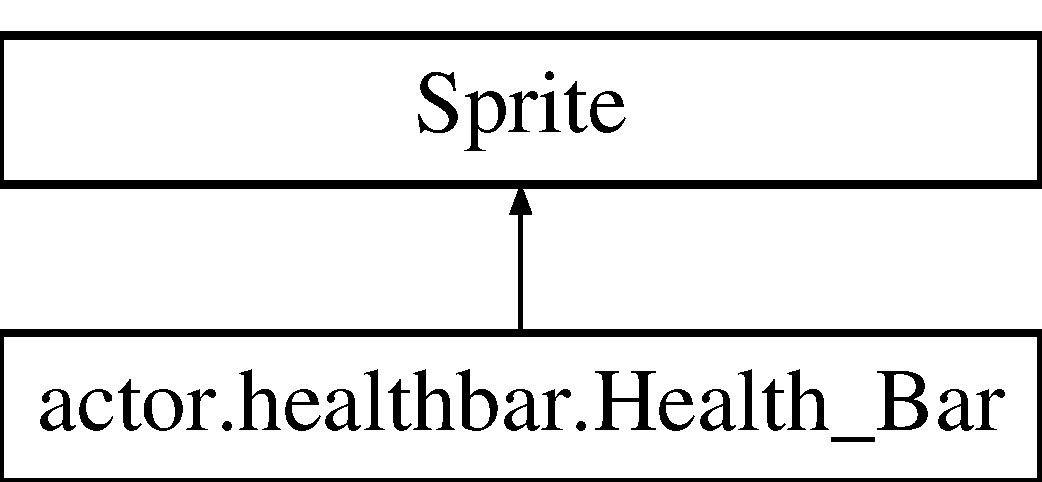
\includegraphics[height=2.000000cm]{classactor_1_1healthbar_1_1_health___bar}
\end{center}
\end{figure}
\subsection*{Public Member Functions}
\begin{DoxyCompactItemize}
\item 
def \hyperlink{classactor_1_1healthbar_1_1_health___bar_a1f35a409c7e1fc7d36600891b7a4a796}{\+\_\+\+\_\+init\+\_\+\+\_\+} (self, x, y)
\begin{DoxyCompactList}\small\item\em Constructor Health\+Bar class. \end{DoxyCompactList}\item 
def \hyperlink{classactor_1_1healthbar_1_1_health___bar_a13d9c179f223a080426841ed336407b5}{health} (self, i)
\begin{DoxyCompactList}\small\item\em Method to update the current sprite image for the healthbar. \end{DoxyCompactList}\end{DoxyCompactItemize}
\subsection*{Public Attributes}
\begin{DoxyCompactItemize}
\item 
\hyperlink{classactor_1_1healthbar_1_1_health___bar_a46e7454053636308c9a17dd63e73a8ee}{image}
\begin{DoxyCompactList}\small\item\em This represents the sprite image for the \hyperlink{classactor_1_1healthbar_1_1_health___bar}{Health\+\_\+\+Bar} object. \end{DoxyCompactList}\item 
\hyperlink{classactor_1_1healthbar_1_1_health___bar_a75ae2266b6d6757be66530b63f413fbd}{h\+\_\+sprite\+\_\+sheet}
\begin{DoxyCompactList}\small\item\em This represents the spritesheet for the image for the \hyperlink{classactor_1_1healthbar_1_1_health___bar}{Health\+\_\+\+Bar} object, containing all sprites associated with the health bar. \end{DoxyCompactList}\item 
\hyperlink{classactor_1_1healthbar_1_1_health___bar_add2392af674af1341a9bef3d18640e83}{rect}
\begin{DoxyCompactList}\small\item\em This represents rectangle for position for the sprite image of the \hyperlink{classactor_1_1healthbar_1_1_health___bar}{Health\+\_\+\+Bar} object. \end{DoxyCompactList}\end{DoxyCompactItemize}


\subsection{Detailed Description}
This class represents the Health\+Bar for the user controlled player character. 

The Health\+Bar class uses the base class for visible game objects from Pygame library. 

\subsection{Constructor \& Destructor Documentation}
\mbox{\Hypertarget{classactor_1_1healthbar_1_1_health___bar_a1f35a409c7e1fc7d36600891b7a4a796}\label{classactor_1_1healthbar_1_1_health___bar_a1f35a409c7e1fc7d36600891b7a4a796}} 
\index{actor\+::healthbar\+::\+Health\+\_\+\+Bar@{actor\+::healthbar\+::\+Health\+\_\+\+Bar}!\+\_\+\+\_\+init\+\_\+\+\_\+@{\+\_\+\+\_\+init\+\_\+\+\_\+}}
\index{\+\_\+\+\_\+init\+\_\+\+\_\+@{\+\_\+\+\_\+init\+\_\+\+\_\+}!actor\+::healthbar\+::\+Health\+\_\+\+Bar@{actor\+::healthbar\+::\+Health\+\_\+\+Bar}}
\subsubsection{\texorpdfstring{\+\_\+\+\_\+init\+\_\+\+\_\+()}{\_\_init\_\_()}}
{\footnotesize\ttfamily def actor.\+healthbar.\+Health\+\_\+\+Bar.\+\_\+\+\_\+init\+\_\+\+\_\+ (\begin{DoxyParamCaption}\item[{}]{self,  }\item[{}]{x,  }\item[{}]{y }\end{DoxyParamCaption})}



Constructor Health\+Bar class. 

Constructor for class initializes the x and y location of the Health\+Bar object. 
\begin{DoxyParams}{Parameters}
{\em x} & this represents the x-\/coordinate at which the Health\+Bar object will be drawn. \\
\hline
{\em y} & this represents the y-\/coordinate at which the Health\+Bar object will be drawn. \\
\hline
\end{DoxyParams}


\subsection{Member Function Documentation}
\mbox{\Hypertarget{classactor_1_1healthbar_1_1_health___bar_a13d9c179f223a080426841ed336407b5}\label{classactor_1_1healthbar_1_1_health___bar_a13d9c179f223a080426841ed336407b5}} 
\index{actor\+::healthbar\+::\+Health\+\_\+\+Bar@{actor\+::healthbar\+::\+Health\+\_\+\+Bar}!health@{health}}
\index{health@{health}!actor\+::healthbar\+::\+Health\+\_\+\+Bar@{actor\+::healthbar\+::\+Health\+\_\+\+Bar}}
\subsubsection{\texorpdfstring{health()}{health()}}
{\footnotesize\ttfamily def actor.\+healthbar.\+Health\+\_\+\+Bar.\+health (\begin{DoxyParamCaption}\item[{}]{self,  }\item[{}]{i }\end{DoxyParamCaption})}



Method to update the current sprite image for the healthbar. 

This method will allow the Health\+Bar to update as soon as the player character is damaged/receives health. 
\begin{DoxyParams}{Parameters}
{\em i} & value represening the number of heart sprites to render to screen. \\
\hline
\end{DoxyParams}


\subsection{Member Data Documentation}
\mbox{\Hypertarget{classactor_1_1healthbar_1_1_health___bar_a75ae2266b6d6757be66530b63f413fbd}\label{classactor_1_1healthbar_1_1_health___bar_a75ae2266b6d6757be66530b63f413fbd}} 
\index{actor\+::healthbar\+::\+Health\+\_\+\+Bar@{actor\+::healthbar\+::\+Health\+\_\+\+Bar}!h\+\_\+sprite\+\_\+sheet@{h\+\_\+sprite\+\_\+sheet}}
\index{h\+\_\+sprite\+\_\+sheet@{h\+\_\+sprite\+\_\+sheet}!actor\+::healthbar\+::\+Health\+\_\+\+Bar@{actor\+::healthbar\+::\+Health\+\_\+\+Bar}}
\subsubsection{\texorpdfstring{h\+\_\+sprite\+\_\+sheet}{h\_sprite\_sheet}}
{\footnotesize\ttfamily actor.\+healthbar.\+Health\+\_\+\+Bar.\+h\+\_\+sprite\+\_\+sheet}



This represents the spritesheet for the image for the \hyperlink{classactor_1_1healthbar_1_1_health___bar}{Health\+\_\+\+Bar} object, containing all sprites associated with the health bar. 

\mbox{\Hypertarget{classactor_1_1healthbar_1_1_health___bar_a46e7454053636308c9a17dd63e73a8ee}\label{classactor_1_1healthbar_1_1_health___bar_a46e7454053636308c9a17dd63e73a8ee}} 
\index{actor\+::healthbar\+::\+Health\+\_\+\+Bar@{actor\+::healthbar\+::\+Health\+\_\+\+Bar}!image@{image}}
\index{image@{image}!actor\+::healthbar\+::\+Health\+\_\+\+Bar@{actor\+::healthbar\+::\+Health\+\_\+\+Bar}}
\subsubsection{\texorpdfstring{image}{image}}
{\footnotesize\ttfamily actor.\+healthbar.\+Health\+\_\+\+Bar.\+image}



This represents the sprite image for the \hyperlink{classactor_1_1healthbar_1_1_health___bar}{Health\+\_\+\+Bar} object. 

\mbox{\Hypertarget{classactor_1_1healthbar_1_1_health___bar_add2392af674af1341a9bef3d18640e83}\label{classactor_1_1healthbar_1_1_health___bar_add2392af674af1341a9bef3d18640e83}} 
\index{actor\+::healthbar\+::\+Health\+\_\+\+Bar@{actor\+::healthbar\+::\+Health\+\_\+\+Bar}!rect@{rect}}
\index{rect@{rect}!actor\+::healthbar\+::\+Health\+\_\+\+Bar@{actor\+::healthbar\+::\+Health\+\_\+\+Bar}}
\subsubsection{\texorpdfstring{rect}{rect}}
{\footnotesize\ttfamily actor.\+healthbar.\+Health\+\_\+\+Bar.\+rect}



This represents rectangle for position for the sprite image of the \hyperlink{classactor_1_1healthbar_1_1_health___bar}{Health\+\_\+\+Bar} object. 



The documentation for this class was generated from the following file\+:\begin{DoxyCompactItemize}
\item 
src/actor/\hyperlink{healthbar_8py}{healthbar.\+py}\end{DoxyCompactItemize}

\hypertarget{classactor_1_1item_1_1_item}{}\section{actor.\+item.\+Item Class Reference}
\label{classactor_1_1item_1_1_item}\index{actor.\+item.\+Item@{actor.\+item.\+Item}}


Consumable \hyperlink{classactor_1_1item_1_1_item}{Item} Class  This class is used for the creation of a random consumable item, spawned once an enemy has been defeated on their last position before despawn.  


Inheritance diagram for actor.\+item.\+Item\+:\begin{figure}[H]
\begin{center}
\leavevmode
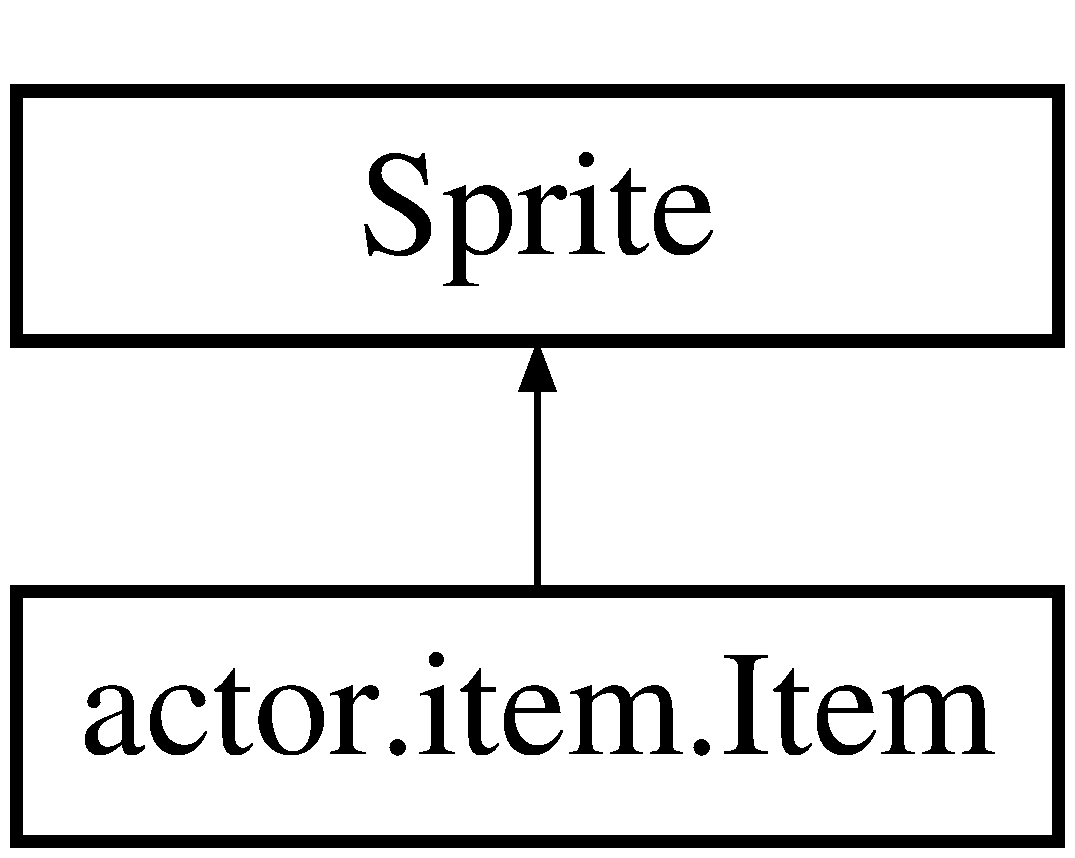
\includegraphics[height=2.000000cm]{classactor_1_1item_1_1_item}
\end{center}
\end{figure}
\subsection*{Public Member Functions}
\begin{DoxyCompactItemize}
\item 
def \hyperlink{classactor_1_1item_1_1_item_a13d4ef784805457c46d4c6872aa0903d}{\+\_\+\+\_\+init\+\_\+\+\_\+} (self, x, y, typ)
\begin{DoxyCompactList}\small\item\em \hyperlink{classactor_1_1item_1_1_item}{Item} constructor  A sprite subclass constructor which takes a pair of x-\/y coordinates, commonly those of the killed enemy, and an item type, in the form of a randomly generated integer from 0 to the \# of possible items. \end{DoxyCompactList}\item 
def \hyperlink{classactor_1_1item_1_1_item_a3ad3940f06483ccce49fe2673896555f}{collision} (self, p)
\begin{DoxyCompactList}\small\item\em Collision handler for the player and the consumable item, depending on the item\textquotesingle{}s type. \end{DoxyCompactList}\end{DoxyCompactItemize}
\subsection*{Public Attributes}
\begin{DoxyCompactItemize}
\item 
\mbox{\Hypertarget{classactor_1_1item_1_1_item_a2f2f0de31fa9a294bdf2c6070c43cf8a}\label{classactor_1_1item_1_1_item_a2f2f0de31fa9a294bdf2c6070c43cf8a}} 
\hyperlink{classactor_1_1item_1_1_item_a2f2f0de31fa9a294bdf2c6070c43cf8a}{image}
\begin{DoxyCompactList}\small\item\em \hyperlink{classactor_1_1item_1_1_item}{Item} sprite image. \end{DoxyCompactList}\item 
\mbox{\Hypertarget{classactor_1_1item_1_1_item_a0341980445d257f74dfc20208a93afd8}\label{classactor_1_1item_1_1_item_a0341980445d257f74dfc20208a93afd8}} 
\hyperlink{classactor_1_1item_1_1_item_a0341980445d257f74dfc20208a93afd8}{itemsprite}
\begin{DoxyCompactList}\small\item\em List of possible item sprite images. \end{DoxyCompactList}\item 
\mbox{\Hypertarget{classactor_1_1item_1_1_item_aebbc33971d663fba6f5bd54e03a63813}\label{classactor_1_1item_1_1_item_aebbc33971d663fba6f5bd54e03a63813}} 
\hyperlink{classactor_1_1item_1_1_item_aebbc33971d663fba6f5bd54e03a63813}{rect}
\begin{DoxyCompactList}\small\item\em \hyperlink{classactor_1_1item_1_1_item}{Item} x and y position. \end{DoxyCompactList}\item 
\mbox{\Hypertarget{classactor_1_1item_1_1_item_aee8f12aa657322ef895d9151dcc54e71}\label{classactor_1_1item_1_1_item_aee8f12aa657322ef895d9151dcc54e71}} 
\hyperlink{classactor_1_1item_1_1_item_aee8f12aa657322ef895d9151dcc54e71}{id}
\begin{DoxyCompactList}\small\item\em Collision ID (how other items tell what this item is) \end{DoxyCompactList}\item 
\mbox{\Hypertarget{classactor_1_1item_1_1_item_ae65791520a3bdb6905e6e14a8b0abb3c}\label{classactor_1_1item_1_1_item_ae65791520a3bdb6905e6e14a8b0abb3c}} 
\hyperlink{classactor_1_1item_1_1_item_ae65791520a3bdb6905e6e14a8b0abb3c}{type}
\begin{DoxyCompactList}\small\item\em Integer value to determine what kind of item this is (rupee, heart, etc) \end{DoxyCompactList}\end{DoxyCompactItemize}


\subsection{Detailed Description}
Consumable \hyperlink{classactor_1_1item_1_1_item}{Item} Class  This class is used for the creation of a random consumable item, spawned once an enemy has been defeated on their last position before despawn. 

\subsection{Constructor \& Destructor Documentation}
\mbox{\Hypertarget{classactor_1_1item_1_1_item_a13d4ef784805457c46d4c6872aa0903d}\label{classactor_1_1item_1_1_item_a13d4ef784805457c46d4c6872aa0903d}} 
\index{actor\+::item\+::\+Item@{actor\+::item\+::\+Item}!\+\_\+\+\_\+init\+\_\+\+\_\+@{\+\_\+\+\_\+init\+\_\+\+\_\+}}
\index{\+\_\+\+\_\+init\+\_\+\+\_\+@{\+\_\+\+\_\+init\+\_\+\+\_\+}!actor\+::item\+::\+Item@{actor\+::item\+::\+Item}}
\subsubsection{\texorpdfstring{\+\_\+\+\_\+init\+\_\+\+\_\+()}{\_\_init\_\_()}}
{\footnotesize\ttfamily def actor.\+item.\+Item.\+\_\+\+\_\+init\+\_\+\+\_\+ (\begin{DoxyParamCaption}\item[{}]{self,  }\item[{}]{x,  }\item[{}]{y,  }\item[{}]{typ }\end{DoxyParamCaption})}



\hyperlink{classactor_1_1item_1_1_item}{Item} constructor  A sprite subclass constructor which takes a pair of x-\/y coordinates, commonly those of the killed enemy, and an item type, in the form of a randomly generated integer from 0 to the \# of possible items. 


\begin{DoxyParams}{Parameters}
{\em x} & X coordinate of the spawned item \\
\hline
{\em y} & Y coordinate of the spawned item \\
\hline
{\em typ} & Integer value to specify the type of consumable item \\
\hline
\end{DoxyParams}


\subsection{Member Function Documentation}
\mbox{\Hypertarget{classactor_1_1item_1_1_item_a3ad3940f06483ccce49fe2673896555f}\label{classactor_1_1item_1_1_item_a3ad3940f06483ccce49fe2673896555f}} 
\index{actor\+::item\+::\+Item@{actor\+::item\+::\+Item}!collision@{collision}}
\index{collision@{collision}!actor\+::item\+::\+Item@{actor\+::item\+::\+Item}}
\subsubsection{\texorpdfstring{collision()}{collision()}}
{\footnotesize\ttfamily def actor.\+item.\+Item.\+collision (\begin{DoxyParamCaption}\item[{}]{self,  }\item[{}]{p }\end{DoxyParamCaption})}



Collision handler for the player and the consumable item, depending on the item\textquotesingle{}s type. 


\begin{DoxyParams}{Parameters}
{\em p} & Player object \\
\hline
\end{DoxyParams}


The documentation for this class was generated from the following file\+:\begin{DoxyCompactItemize}
\item 
src/actor/\hyperlink{item_8py}{item.\+py}\end{DoxyCompactItemize}

\hypertarget{classactor_1_1keese_1_1_keese}{}\section{actor.\+keese.\+Keese Class Reference}
\label{classactor_1_1keese_1_1_keese}\index{actor.\+keese.\+Keese@{actor.\+keese.\+Keese}}


This class represents the \hyperlink{classactor_1_1keese_1_1_keese}{Keese} enemy.  


Inheritance diagram for actor.\+keese.\+Keese\+:\begin{figure}[H]
\begin{center}
\leavevmode
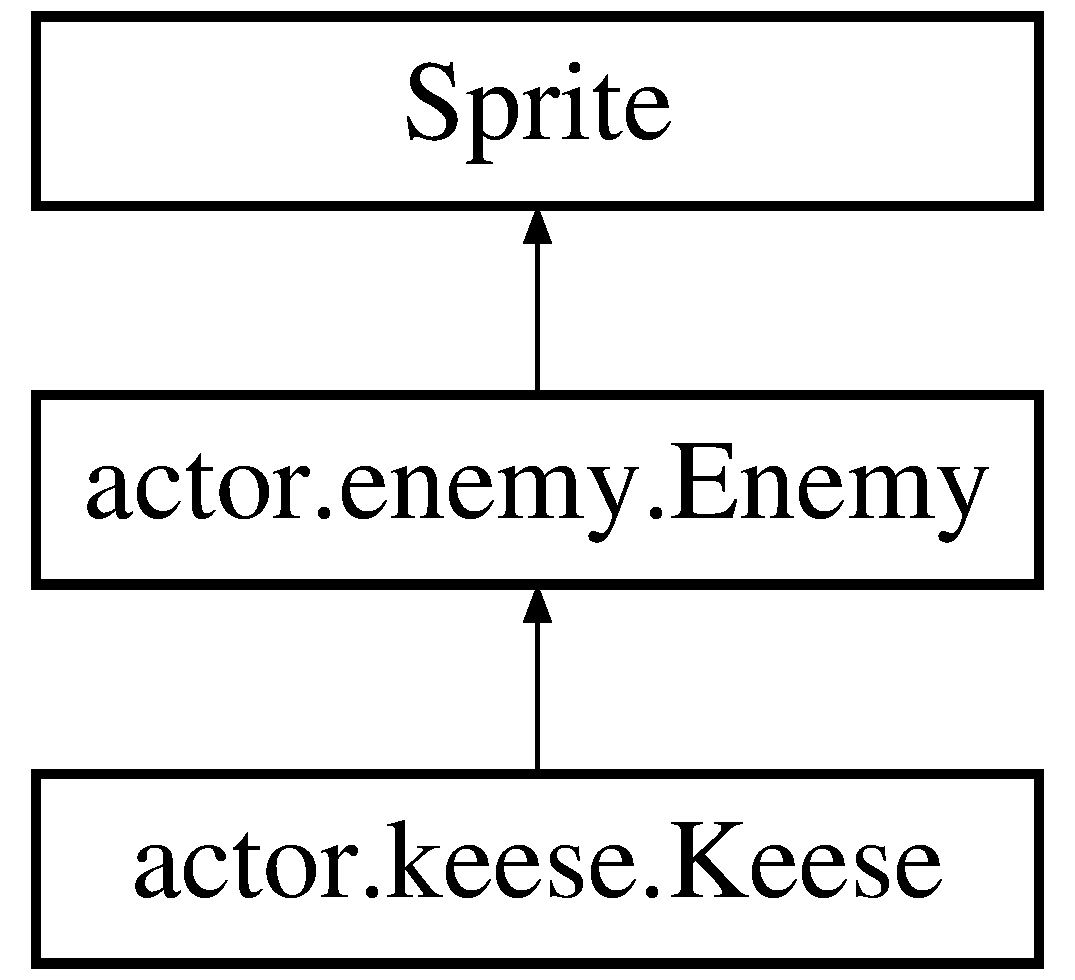
\includegraphics[height=3.000000cm]{classactor_1_1keese_1_1_keese}
\end{center}
\end{figure}
\subsection*{Public Member Functions}
\begin{DoxyCompactItemize}
\item 
def \hyperlink{classactor_1_1keese_1_1_keese_a5a6d46ac05ff7500ab07e0494ddbe3ce}{\+\_\+\+\_\+init\+\_\+\+\_\+} (self, x, y)
\begin{DoxyCompactList}\small\item\em Constructor for \hyperlink{classactor_1_1keese_1_1_keese}{Keese}. \end{DoxyCompactList}\item 
def \hyperlink{classactor_1_1keese_1_1_keese_ad69c85211ff8008fd3c223296dc16af7}{gen\+Rest\+Length} (self)
\begin{DoxyCompactList}\small\item\em Sets the \hyperlink{classactor_1_1keese_1_1_keese}{Keese} rest length. \end{DoxyCompactList}\item 
def \hyperlink{classactor_1_1keese_1_1_keese_a7abbd03624a6695b83d3086e48957d86}{gen\+Travel\+Point} (self)
\begin{DoxyCompactList}\small\item\em Creates a new travel point for \hyperlink{classactor_1_1keese_1_1_keese}{Keese}. \end{DoxyCompactList}\item 
def \hyperlink{classactor_1_1keese_1_1_keese_aee33f864229b0a7aa9a8b1d258ed696b}{switch\+Sprite} (self)
\begin{DoxyCompactList}\small\item\em Iterates through the sprite list. \end{DoxyCompactList}\item 
def \hyperlink{classactor_1_1keese_1_1_keese_a61477e66e28a62bb0a72a302b13c3ca0}{stop} (self)
\begin{DoxyCompactList}\small\item\em Stops the \hyperlink{classactor_1_1keese_1_1_keese}{Keese}. \end{DoxyCompactList}\item 
def \hyperlink{classactor_1_1keese_1_1_keese_a6fe0305b143de210b4b161a1091f7891}{set\+Move\+Speed} (self)
\begin{DoxyCompactList}\small\item\em Sets the \hyperlink{classactor_1_1keese_1_1_keese}{Keese} x and y movement speed. \end{DoxyCompactList}\item 
def \hyperlink{classactor_1_1keese_1_1_keese_a2c191c26fc310458619fdf49166e8434}{check\+State} (self)
\begin{DoxyCompactList}\small\item\em Evaluates the state of the \hyperlink{classactor_1_1keese_1_1_keese}{Keese}. \end{DoxyCompactList}\item 
def \hyperlink{classactor_1_1keese_1_1_keese_a838343717716ba48c0519e73d702cac9}{enemy\+Logic} (self)
\begin{DoxyCompactList}\small\item\em Controls \hyperlink{classactor_1_1keese_1_1_keese}{Keese} logic. \end{DoxyCompactList}\end{DoxyCompactItemize}
\subsection*{Public Attributes}
\begin{DoxyCompactItemize}
\item 
\mbox{\Hypertarget{classactor_1_1keese_1_1_keese_a65676a0ae6de92c1731dfa30ce354372}\label{classactor_1_1keese_1_1_keese_a65676a0ae6de92c1731dfa30ce354372}} 
\hyperlink{classactor_1_1keese_1_1_keese_a65676a0ae6de92c1731dfa30ce354372}{is\+Moving}
\begin{DoxyCompactList}\small\item\em Whether the \hyperlink{classactor_1_1keese_1_1_keese}{Keese} is moving. \end{DoxyCompactList}\item 
\mbox{\Hypertarget{classactor_1_1keese_1_1_keese_afd916a8c02ccf5ac8a28f87f67b67d9d}\label{classactor_1_1keese_1_1_keese_afd916a8c02ccf5ac8a28f87f67b67d9d}} 
\hyperlink{classactor_1_1keese_1_1_keese_afd916a8c02ccf5ac8a28f87f67b67d9d}{can\+Stop}
\begin{DoxyCompactList}\small\item\em Whether the \hyperlink{classactor_1_1keese_1_1_keese}{Keese} can stop. \end{DoxyCompactList}\item 
\mbox{\Hypertarget{classactor_1_1keese_1_1_keese_a38eccba4aae77109933d668223e5948c}\label{classactor_1_1keese_1_1_keese_a38eccba4aae77109933d668223e5948c}} 
\hyperlink{classactor_1_1keese_1_1_keese_a38eccba4aae77109933d668223e5948c}{is\+Resting}
\begin{DoxyCompactList}\small\item\em Whether the Keees is resting. \end{DoxyCompactList}\item 
\mbox{\Hypertarget{classactor_1_1keese_1_1_keese_ab98be6a25c06f1e149ff22c90a6937c9}\label{classactor_1_1keese_1_1_keese_ab98be6a25c06f1e149ff22c90a6937c9}} 
\hyperlink{classactor_1_1keese_1_1_keese_ab98be6a25c06f1e149ff22c90a6937c9}{travel\+Point}
\begin{DoxyCompactList}\small\item\em Point the \hyperlink{classactor_1_1keese_1_1_keese}{Keese} is traveling to. \end{DoxyCompactList}\item 
\mbox{\Hypertarget{classactor_1_1keese_1_1_keese_a547b4c212a286e288e38256351776a97}\label{classactor_1_1keese_1_1_keese_a547b4c212a286e288e38256351776a97}} 
\hyperlink{classactor_1_1keese_1_1_keese_a547b4c212a286e288e38256351776a97}{rest\+Time}
\begin{DoxyCompactList}\small\item\em The amount of frames the \hyperlink{classactor_1_1keese_1_1_keese}{Keese} will rest for. \end{DoxyCompactList}\item 
\mbox{\Hypertarget{classactor_1_1keese_1_1_keese_ab4569cac512e0ee58ace7bdc0e71ea8a}\label{classactor_1_1keese_1_1_keese_ab4569cac512e0ee58ace7bdc0e71ea8a}} 
\hyperlink{classactor_1_1keese_1_1_keese_ab4569cac512e0ee58ace7bdc0e71ea8a}{rest\+Start\+Frame}
\begin{DoxyCompactList}\small\item\em The frame the \hyperlink{classactor_1_1keese_1_1_keese}{Keese} starts resting. \end{DoxyCompactList}\item 
\mbox{\Hypertarget{classactor_1_1keese_1_1_keese_a9ecd9b101873fd64a9406ebd550dc761}\label{classactor_1_1keese_1_1_keese_a9ecd9b101873fd64a9406ebd550dc761}} 
\hyperlink{classactor_1_1keese_1_1_keese_a9ecd9b101873fd64a9406ebd550dc761}{fly\+Start\+Frame}
\begin{DoxyCompactList}\small\item\em The frame the \hyperlink{classactor_1_1keese_1_1_keese}{Keese} starts flying on. \end{DoxyCompactList}\item 
\mbox{\Hypertarget{classactor_1_1keese_1_1_keese_a9931a961d40612b60a09eec8607198a4}\label{classactor_1_1keese_1_1_keese_a9931a961d40612b60a09eec8607198a4}} 
\hyperlink{classactor_1_1keese_1_1_keese_a9931a961d40612b60a09eec8607198a4}{sprite\+Index}
\begin{DoxyCompactList}\small\item\em The sprite list index. \end{DoxyCompactList}\item 
\mbox{\Hypertarget{classactor_1_1keese_1_1_keese_a30dd6801255414be0d18fdba0f321bca}\label{classactor_1_1keese_1_1_keese_a30dd6801255414be0d18fdba0f321bca}} 
\hyperlink{classactor_1_1keese_1_1_keese_a30dd6801255414be0d18fdba0f321bca}{max\+HP}
\begin{DoxyCompactList}\small\item\em \hyperlink{classactor_1_1keese_1_1_keese}{Keese} max health. \end{DoxyCompactList}\item 
\mbox{\Hypertarget{classactor_1_1keese_1_1_keese_a41e62f021c65cd05dc748e265265be71}\label{classactor_1_1keese_1_1_keese_a41e62f021c65cd05dc748e265265be71}} 
\hyperlink{classactor_1_1keese_1_1_keese_a41e62f021c65cd05dc748e265265be71}{HP}
\begin{DoxyCompactList}\small\item\em \hyperlink{classactor_1_1keese_1_1_keese}{Keese} current health. \end{DoxyCompactList}\item 
\mbox{\Hypertarget{classactor_1_1keese_1_1_keese_a2698d3b6a02884479d1613d236618728}\label{classactor_1_1keese_1_1_keese_a2698d3b6a02884479d1613d236618728}} 
\hyperlink{classactor_1_1keese_1_1_keese_a2698d3b6a02884479d1613d236618728}{dmg}
\begin{DoxyCompactList}\small\item\em \hyperlink{classactor_1_1keese_1_1_keese}{Keese} damage. \end{DoxyCompactList}\item 
\hyperlink{classactor_1_1keese_1_1_keese_ae61225fd17e93f8441dae1eef5e41538}{image}
\begin{DoxyCompactList}\small\item\em \hyperlink{classactor_1_1keese_1_1_keese}{Keese} current sprite. \end{DoxyCompactList}\item 
\mbox{\Hypertarget{classactor_1_1keese_1_1_keese_a0217078fcd7416adddc4d3671c3a653e}\label{classactor_1_1keese_1_1_keese_a0217078fcd7416adddc4d3671c3a653e}} 
\hyperlink{classactor_1_1keese_1_1_keese_a0217078fcd7416adddc4d3671c3a653e}{sprites}
\begin{DoxyCompactList}\small\item\em \hyperlink{classactor_1_1keese_1_1_keese}{Keese} sprite list. \end{DoxyCompactList}\item 
\hyperlink{classactor_1_1keese_1_1_keese_a4d93a0d3f92f4e23517b90e538d40467}{x\+Speed}
\begin{DoxyCompactList}\small\item\em The current x-\/directional speed for \hyperlink{classactor_1_1keese_1_1_keese}{Keese} in movement/stationary state. \end{DoxyCompactList}\item 
\hyperlink{classactor_1_1keese_1_1_keese_a6a288010700b821bc27840aa94faf35f}{y\+Speed}
\begin{DoxyCompactList}\small\item\em The current y-\/directional speed for \hyperlink{classactor_1_1keese_1_1_keese}{Keese} in movement/stationary state. \end{DoxyCompactList}\item 
\hyperlink{classactor_1_1keese_1_1_keese_a4cb2d09574c5b9590ea9f9d30c942a16}{hit\+Count}
\begin{DoxyCompactList}\small\item\em Integer value representing the buffer for the number of hits for \hyperlink{classactor_1_1keese_1_1_keese}{Keese} after being hit by player character. \end{DoxyCompactList}\item 
\hyperlink{classactor_1_1keese_1_1_keese_a88d77dbe81f2a8ab5e25bfb8bb1b2ae7}{is\+Hit}
\begin{DoxyCompactList}\small\item\em Represents the current state if \hyperlink{classactor_1_1keese_1_1_keese}{Keese} has collided with player character attack. \end{DoxyCompactList}\end{DoxyCompactItemize}


\subsection{Detailed Description}
This class represents the \hyperlink{classactor_1_1keese_1_1_keese}{Keese} enemy. 

\subsection{Constructor \& Destructor Documentation}
\mbox{\Hypertarget{classactor_1_1keese_1_1_keese_a5a6d46ac05ff7500ab07e0494ddbe3ce}\label{classactor_1_1keese_1_1_keese_a5a6d46ac05ff7500ab07e0494ddbe3ce}} 
\index{actor\+::keese\+::\+Keese@{actor\+::keese\+::\+Keese}!\+\_\+\+\_\+init\+\_\+\+\_\+@{\+\_\+\+\_\+init\+\_\+\+\_\+}}
\index{\+\_\+\+\_\+init\+\_\+\+\_\+@{\+\_\+\+\_\+init\+\_\+\+\_\+}!actor\+::keese\+::\+Keese@{actor\+::keese\+::\+Keese}}
\subsubsection{\texorpdfstring{\+\_\+\+\_\+init\+\_\+\+\_\+()}{\_\_init\_\_()}}
{\footnotesize\ttfamily def actor.\+keese.\+Keese.\+\_\+\+\_\+init\+\_\+\+\_\+ (\begin{DoxyParamCaption}\item[{}]{self,  }\item[{}]{x,  }\item[{}]{y }\end{DoxyParamCaption})}



Constructor for \hyperlink{classactor_1_1keese_1_1_keese}{Keese}. 

Constructor takes two parameters, the x and y coordinates 
\begin{DoxyParams}{Parameters}
{\em x} & X coordinate of the starting postion of the \hyperlink{classactor_1_1keese_1_1_keese}{Keese} \\
\hline
{\em y} & Y coordinate of the starting postion of the \hyperlink{classactor_1_1keese_1_1_keese}{Keese} \\
\hline
\end{DoxyParams}


\subsection{Member Function Documentation}
\mbox{\Hypertarget{classactor_1_1keese_1_1_keese_a2c191c26fc310458619fdf49166e8434}\label{classactor_1_1keese_1_1_keese_a2c191c26fc310458619fdf49166e8434}} 
\index{actor\+::keese\+::\+Keese@{actor\+::keese\+::\+Keese}!check\+State@{check\+State}}
\index{check\+State@{check\+State}!actor\+::keese\+::\+Keese@{actor\+::keese\+::\+Keese}}
\subsubsection{\texorpdfstring{check\+State()}{checkState()}}
{\footnotesize\ttfamily def actor.\+keese.\+Keese.\+check\+State (\begin{DoxyParamCaption}\item[{}]{self }\end{DoxyParamCaption})}



Evaluates the state of the \hyperlink{classactor_1_1keese_1_1_keese}{Keese}. 

Evalautes if the \hyperlink{classactor_1_1keese_1_1_keese}{Keese} if moving, if it can stop, if it is in iframes, and if it has died \mbox{\Hypertarget{classactor_1_1keese_1_1_keese_a838343717716ba48c0519e73d702cac9}\label{classactor_1_1keese_1_1_keese_a838343717716ba48c0519e73d702cac9}} 
\index{actor\+::keese\+::\+Keese@{actor\+::keese\+::\+Keese}!enemy\+Logic@{enemy\+Logic}}
\index{enemy\+Logic@{enemy\+Logic}!actor\+::keese\+::\+Keese@{actor\+::keese\+::\+Keese}}
\subsubsection{\texorpdfstring{enemy\+Logic()}{enemyLogic()}}
{\footnotesize\ttfamily def actor.\+keese.\+Keese.\+enemy\+Logic (\begin{DoxyParamCaption}\item[{}]{self }\end{DoxyParamCaption})}



Controls \hyperlink{classactor_1_1keese_1_1_keese}{Keese} logic. 

Uses the states to control the \hyperlink{classactor_1_1keese_1_1_keese}{Keese} \mbox{\Hypertarget{classactor_1_1keese_1_1_keese_ad69c85211ff8008fd3c223296dc16af7}\label{classactor_1_1keese_1_1_keese_ad69c85211ff8008fd3c223296dc16af7}} 
\index{actor\+::keese\+::\+Keese@{actor\+::keese\+::\+Keese}!gen\+Rest\+Length@{gen\+Rest\+Length}}
\index{gen\+Rest\+Length@{gen\+Rest\+Length}!actor\+::keese\+::\+Keese@{actor\+::keese\+::\+Keese}}
\subsubsection{\texorpdfstring{gen\+Rest\+Length()}{genRestLength()}}
{\footnotesize\ttfamily def actor.\+keese.\+Keese.\+gen\+Rest\+Length (\begin{DoxyParamCaption}\item[{}]{self }\end{DoxyParamCaption})}



Sets the \hyperlink{classactor_1_1keese_1_1_keese}{Keese} rest length. 

Generates a random number between \mbox{[}1,2\mbox{]} inclusive as the rest time between movements and sets the rest start frame to the current frame \mbox{\Hypertarget{classactor_1_1keese_1_1_keese_a7abbd03624a6695b83d3086e48957d86}\label{classactor_1_1keese_1_1_keese_a7abbd03624a6695b83d3086e48957d86}} 
\index{actor\+::keese\+::\+Keese@{actor\+::keese\+::\+Keese}!gen\+Travel\+Point@{gen\+Travel\+Point}}
\index{gen\+Travel\+Point@{gen\+Travel\+Point}!actor\+::keese\+::\+Keese@{actor\+::keese\+::\+Keese}}
\subsubsection{\texorpdfstring{gen\+Travel\+Point()}{genTravelPoint()}}
{\footnotesize\ttfamily def actor.\+keese.\+Keese.\+gen\+Travel\+Point (\begin{DoxyParamCaption}\item[{}]{self }\end{DoxyParamCaption})}



Creates a new travel point for \hyperlink{classactor_1_1keese_1_1_keese}{Keese}. 

Generate a random point to move to between 0 an the width -\/ 30 of the screen for the x coordinate and between 0 and the height -\/ 30 of the screen for the y coordinate \mbox{\Hypertarget{classactor_1_1keese_1_1_keese_a6fe0305b143de210b4b161a1091f7891}\label{classactor_1_1keese_1_1_keese_a6fe0305b143de210b4b161a1091f7891}} 
\index{actor\+::keese\+::\+Keese@{actor\+::keese\+::\+Keese}!set\+Move\+Speed@{set\+Move\+Speed}}
\index{set\+Move\+Speed@{set\+Move\+Speed}!actor\+::keese\+::\+Keese@{actor\+::keese\+::\+Keese}}
\subsubsection{\texorpdfstring{set\+Move\+Speed()}{setMoveSpeed()}}
{\footnotesize\ttfamily def actor.\+keese.\+Keese.\+set\+Move\+Speed (\begin{DoxyParamCaption}\item[{}]{self }\end{DoxyParamCaption})}



Sets the \hyperlink{classactor_1_1keese_1_1_keese}{Keese} x and y movement speed. 

Compares the two lengths of travel (x and y) and sets the speed in which ever direction is longer to the max speed and the other to a scalar multiple of the max speed based on the ratio of the two lengths \mbox{\Hypertarget{classactor_1_1keese_1_1_keese_a61477e66e28a62bb0a72a302b13c3ca0}\label{classactor_1_1keese_1_1_keese_a61477e66e28a62bb0a72a302b13c3ca0}} 
\index{actor\+::keese\+::\+Keese@{actor\+::keese\+::\+Keese}!stop@{stop}}
\index{stop@{stop}!actor\+::keese\+::\+Keese@{actor\+::keese\+::\+Keese}}
\subsubsection{\texorpdfstring{stop()}{stop()}}
{\footnotesize\ttfamily def actor.\+keese.\+Keese.\+stop (\begin{DoxyParamCaption}\item[{}]{self }\end{DoxyParamCaption})}



Stops the \hyperlink{classactor_1_1keese_1_1_keese}{Keese}. 

Sets the \hyperlink{classactor_1_1keese_1_1_keese}{Keese} speed in the x direction and the y direction to zero \mbox{\Hypertarget{classactor_1_1keese_1_1_keese_aee33f864229b0a7aa9a8b1d258ed696b}\label{classactor_1_1keese_1_1_keese_aee33f864229b0a7aa9a8b1d258ed696b}} 
\index{actor\+::keese\+::\+Keese@{actor\+::keese\+::\+Keese}!switch\+Sprite@{switch\+Sprite}}
\index{switch\+Sprite@{switch\+Sprite}!actor\+::keese\+::\+Keese@{actor\+::keese\+::\+Keese}}
\subsubsection{\texorpdfstring{switch\+Sprite()}{switchSprite()}}
{\footnotesize\ttfamily def actor.\+keese.\+Keese.\+switch\+Sprite (\begin{DoxyParamCaption}\item[{}]{self }\end{DoxyParamCaption})}



Iterates through the sprite list. 

Swaps between the two sprites that are avalible for the keese 

\subsection{Member Data Documentation}
\mbox{\Hypertarget{classactor_1_1keese_1_1_keese_a4cb2d09574c5b9590ea9f9d30c942a16}\label{classactor_1_1keese_1_1_keese_a4cb2d09574c5b9590ea9f9d30c942a16}} 
\index{actor\+::keese\+::\+Keese@{actor\+::keese\+::\+Keese}!hit\+Count@{hit\+Count}}
\index{hit\+Count@{hit\+Count}!actor\+::keese\+::\+Keese@{actor\+::keese\+::\+Keese}}
\subsubsection{\texorpdfstring{hit\+Count}{hitCount}}
{\footnotesize\ttfamily actor.\+keese.\+Keese.\+hit\+Count}



Integer value representing the buffer for the number of hits for \hyperlink{classactor_1_1keese_1_1_keese}{Keese} after being hit by player character. 

\mbox{\Hypertarget{classactor_1_1keese_1_1_keese_ae61225fd17e93f8441dae1eef5e41538}\label{classactor_1_1keese_1_1_keese_ae61225fd17e93f8441dae1eef5e41538}} 
\index{actor\+::keese\+::\+Keese@{actor\+::keese\+::\+Keese}!image@{image}}
\index{image@{image}!actor\+::keese\+::\+Keese@{actor\+::keese\+::\+Keese}}
\subsubsection{\texorpdfstring{image}{image}}
{\footnotesize\ttfamily actor.\+keese.\+Keese.\+image}



\hyperlink{classactor_1_1keese_1_1_keese}{Keese} current sprite. 

Set \hyperlink{classactor_1_1keese_1_1_keese}{Keese} starting sprite. \mbox{\Hypertarget{classactor_1_1keese_1_1_keese_a88d77dbe81f2a8ab5e25bfb8bb1b2ae7}\label{classactor_1_1keese_1_1_keese_a88d77dbe81f2a8ab5e25bfb8bb1b2ae7}} 
\index{actor\+::keese\+::\+Keese@{actor\+::keese\+::\+Keese}!is\+Hit@{is\+Hit}}
\index{is\+Hit@{is\+Hit}!actor\+::keese\+::\+Keese@{actor\+::keese\+::\+Keese}}
\subsubsection{\texorpdfstring{is\+Hit}{isHit}}
{\footnotesize\ttfamily actor.\+keese.\+Keese.\+is\+Hit}



Represents the current state if \hyperlink{classactor_1_1keese_1_1_keese}{Keese} has collided with player character attack. 

\mbox{\Hypertarget{classactor_1_1keese_1_1_keese_a4d93a0d3f92f4e23517b90e538d40467}\label{classactor_1_1keese_1_1_keese_a4d93a0d3f92f4e23517b90e538d40467}} 
\index{actor\+::keese\+::\+Keese@{actor\+::keese\+::\+Keese}!x\+Speed@{x\+Speed}}
\index{x\+Speed@{x\+Speed}!actor\+::keese\+::\+Keese@{actor\+::keese\+::\+Keese}}
\subsubsection{\texorpdfstring{x\+Speed}{xSpeed}}
{\footnotesize\ttfamily actor.\+keese.\+Keese.\+x\+Speed}



The current x-\/directional speed for \hyperlink{classactor_1_1keese_1_1_keese}{Keese} in movement/stationary state. 

\mbox{\Hypertarget{classactor_1_1keese_1_1_keese_a6a288010700b821bc27840aa94faf35f}\label{classactor_1_1keese_1_1_keese_a6a288010700b821bc27840aa94faf35f}} 
\index{actor\+::keese\+::\+Keese@{actor\+::keese\+::\+Keese}!y\+Speed@{y\+Speed}}
\index{y\+Speed@{y\+Speed}!actor\+::keese\+::\+Keese@{actor\+::keese\+::\+Keese}}
\subsubsection{\texorpdfstring{y\+Speed}{ySpeed}}
{\footnotesize\ttfamily actor.\+keese.\+Keese.\+y\+Speed}



The current y-\/directional speed for \hyperlink{classactor_1_1keese_1_1_keese}{Keese} in movement/stationary state. 



The documentation for this class was generated from the following file\+:\begin{DoxyCompactItemize}
\item 
src/actor/\hyperlink{keese_8py}{keese.\+py}\end{DoxyCompactItemize}

\hypertarget{classcollision_1_1level_1_1_level}{}\section{collision.\+level.\+Level Class Reference}
\label{classcollision_1_1level_1_1_level}\index{collision.\+level.\+Level@{collision.\+level.\+Level}}


Dungeon level background class  Creates the background of a dungeon, can be modified in the future to change colour based on sprite sheet and new arg.  


Inheritance diagram for collision.\+level.\+Level\+:\begin{figure}[H]
\begin{center}
\leavevmode
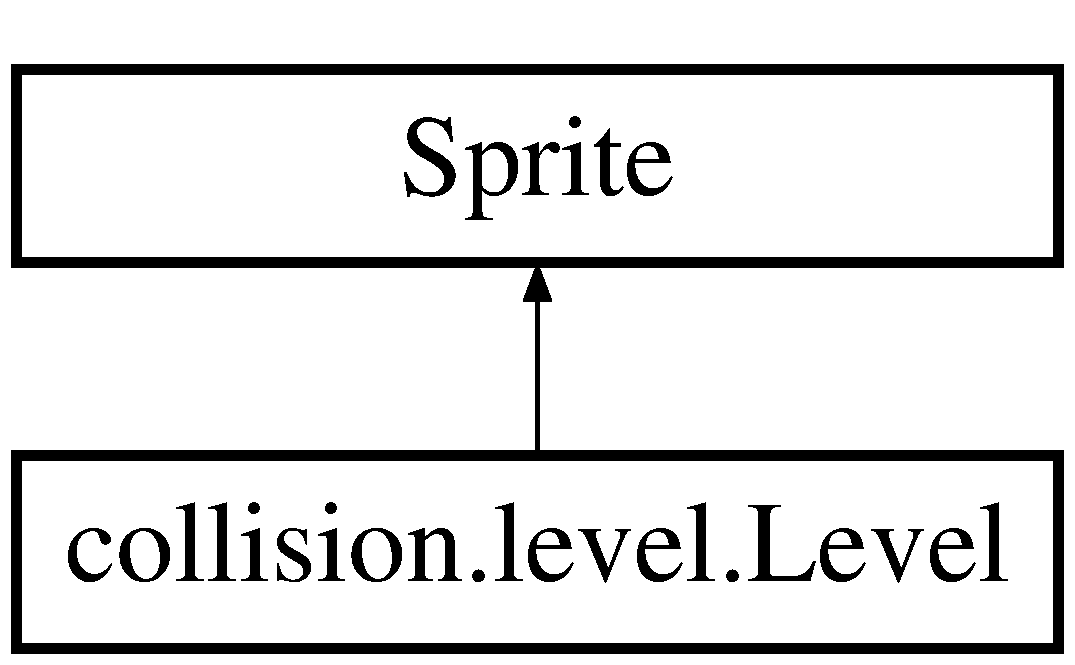
\includegraphics[height=2.000000cm]{classcollision_1_1level_1_1_level}
\end{center}
\end{figure}
\subsection*{Public Member Functions}
\begin{DoxyCompactItemize}
\item 
\mbox{\Hypertarget{classcollision_1_1level_1_1_level_a241b5e528c34fdcfe53f70c0041bea2a}\label{classcollision_1_1level_1_1_level_a241b5e528c34fdcfe53f70c0041bea2a}} 
def \hyperlink{classcollision_1_1level_1_1_level_a241b5e528c34fdcfe53f70c0041bea2a}{\+\_\+\+\_\+init\+\_\+\+\_\+} (self)
\begin{DoxyCompactList}\small\item\em Background initializer  Initialize a background to constantly be printed as game background. \end{DoxyCompactList}\end{DoxyCompactItemize}
\subsection*{Public Attributes}
\begin{DoxyCompactItemize}
\item 
\mbox{\Hypertarget{classcollision_1_1level_1_1_level_a6be6fa8fdddb3acd8c632933afaa1bd4}\label{classcollision_1_1level_1_1_level_a6be6fa8fdddb3acd8c632933afaa1bd4}} 
\hyperlink{classcollision_1_1level_1_1_level_a6be6fa8fdddb3acd8c632933afaa1bd4}{image}
\begin{DoxyCompactList}\small\item\em \hyperlink{classcollision_1_1level_1_1_level}{Level} background sprite image. \end{DoxyCompactList}\item 
\mbox{\Hypertarget{classcollision_1_1level_1_1_level_a8f353b28bfe30c913bb5806d8eff5d54}\label{classcollision_1_1level_1_1_level_a8f353b28bfe30c913bb5806d8eff5d54}} 
\hyperlink{classcollision_1_1level_1_1_level_a8f353b28bfe30c913bb5806d8eff5d54}{rect}
\begin{DoxyCompactList}\small\item\em Background x and y coordinates (adjusted for the H\+UD display) \end{DoxyCompactList}\end{DoxyCompactItemize}


\subsection{Detailed Description}
Dungeon level background class  Creates the background of a dungeon, can be modified in the future to change colour based on sprite sheet and new arg. 

The documentation for this class was generated from the following file\+:\begin{DoxyCompactItemize}
\item 
src/collision/\hyperlink{level_8py}{level.\+py}\end{DoxyCompactItemize}

\hypertarget{classcollision_1_1levelmanager_1_1_level_manager}{}\section{collision.\+levelmanager.\+Level\+Manager Class Reference}
\label{classcollision_1_1levelmanager_1_1_level_manager}\index{collision.\+levelmanager.\+Level\+Manager@{collision.\+levelmanager.\+Level\+Manager}}


Dungeon Level Creation Class  Class used as a master constructor for every dungeon levels, getting pre-\/written data and loading it when the game starts and when a transition occurs.  


\subsection*{Public Member Functions}
\begin{DoxyCompactItemize}
\item 
def \hyperlink{classcollision_1_1levelmanager_1_1_level_manager_ac15451905c2523ed3929d877762bb290}{\+\_\+\+\_\+init\+\_\+\+\_\+} (self, spritelist, collidlist, updatelist)
\begin{DoxyCompactList}\small\item\em Dungeon Level Master Initializer  The class initializer, taking empty lists, each for letting the \hyperlink{classcollision_1_1levelmanager_1_1_level_manager_a02aa3ee9b35d68c9386517c518c101f4}{make()} function define what objects need to be drawn/collidable/updatable. \end{DoxyCompactList}\item 
def \hyperlink{classcollision_1_1levelmanager_1_1_level_manager_a02aa3ee9b35d68c9386517c518c101f4}{make} (self, \hyperlink{classcollision_1_1levelmanager_1_1_level_manager_a5d1c987dbd37f1da1496915d4a754d70}{x}, \hyperlink{classcollision_1_1levelmanager_1_1_level_manager_a5b6011487a9ea527e43194554dbf1326}{y})
\begin{DoxyCompactList}\small\item\em Dungeon Level Constructor  The main function to load a given index of data from leveldata.\+py, and load it into the game environment. \end{DoxyCompactList}\item 
def \hyperlink{classcollision_1_1levelmanager_1_1_level_manager_ac73f0ef69a1d1ff85a906a68cb1e2c86}{transition} (self, xchange, ychange)
\begin{DoxyCompactList}\small\item\em Dungeon level transition function, used to go to an adjacent level, clear all current data, and load new room data. \end{DoxyCompactList}\item 
\mbox{\Hypertarget{classcollision_1_1levelmanager_1_1_level_manager_a5eb6314d72a5b6a438eb85ef1a926ce0}\label{classcollision_1_1levelmanager_1_1_level_manager_a5eb6314d72a5b6a438eb85ef1a926ce0}} 
def \hyperlink{classcollision_1_1levelmanager_1_1_level_manager_a5eb6314d72a5b6a438eb85ef1a926ce0}{open} (self)
\begin{DoxyCompactList}\small\item\em Function to open all blocked doors in the current dungeon room (usually used when all enemies defeated, locked doors stay locked) \end{DoxyCompactList}\item 
\mbox{\Hypertarget{classcollision_1_1levelmanager_1_1_level_manager_ab31d4ea306a0ef50bf25a4a4dd3b9aaf}\label{classcollision_1_1levelmanager_1_1_level_manager_ab31d4ea306a0ef50bf25a4a4dd3b9aaf}} 
def \hyperlink{classcollision_1_1levelmanager_1_1_level_manager_ab31d4ea306a0ef50bf25a4a4dd3b9aaf}{endroom} (self)
\begin{DoxyCompactList}\small\item\em Function to store current data, open all blocked doors, and possibly spawn a key/prize when all enemies defeated  When all enemies in a room are killed, this function is called, changing the enemy array in leveldata.\+py for the current level to an empty array (so enemies don\textquotesingle{}t reload once you enter again), running the self.\+open() function to open all blocked doors, and if the room\+ID is a predetermined key/rupy room, spawn a key/rupy in the middle of the room. \end{DoxyCompactList}\item 
\mbox{\Hypertarget{classcollision_1_1levelmanager_1_1_level_manager_a11bb309e2c9c137a0000f1d94b3788f6}\label{classcollision_1_1levelmanager_1_1_level_manager_a11bb309e2c9c137a0000f1d94b3788f6}} 
def \hyperlink{classcollision_1_1levelmanager_1_1_level_manager_a11bb309e2c9c137a0000f1d94b3788f6}{clear} (self)
\begin{DoxyCompactList}\small\item\em Clears the levelmanager\textquotesingle{}s update lists  Empty all sprite lists for the game (spritelist, collisionlist, and updatelist), usually used in transition from one room to another. \end{DoxyCompactList}\end{DoxyCompactItemize}
\subsection*{Public Attributes}
\begin{DoxyCompactItemize}
\item 
\mbox{\Hypertarget{classcollision_1_1levelmanager_1_1_level_manager_a05b0081f0ceb5ff238e29476d26f5bc5}\label{classcollision_1_1levelmanager_1_1_level_manager_a05b0081f0ceb5ff238e29476d26f5bc5}} 
\hyperlink{classcollision_1_1levelmanager_1_1_level_manager_a05b0081f0ceb5ff238e29476d26f5bc5}{sl}
\begin{DoxyCompactList}\small\item\em List of objects to be printed (ie player, not invisible walls) \end{DoxyCompactList}\item 
\mbox{\Hypertarget{classcollision_1_1levelmanager_1_1_level_manager_af2f247df791be0e0a8d1adc357e679b4}\label{classcollision_1_1levelmanager_1_1_level_manager_af2f247df791be0e0a8d1adc357e679b4}} 
\hyperlink{classcollision_1_1levelmanager_1_1_level_manager_af2f247df791be0e0a8d1adc357e679b4}{cl}
\begin{DoxyCompactList}\small\item\em List of objects that can be collided with (ie keese, not level background) \end{DoxyCompactList}\item 
\mbox{\Hypertarget{classcollision_1_1levelmanager_1_1_level_manager_a612895753b85eced72f425f4f23885fd}\label{classcollision_1_1levelmanager_1_1_level_manager_a612895753b85eced72f425f4f23885fd}} 
\hyperlink{classcollision_1_1levelmanager_1_1_level_manager_a612895753b85eced72f425f4f23885fd}{ul}
\begin{DoxyCompactList}\small\item\em List of objects that need to be constantly updated (ie player, not walls/static objects) \end{DoxyCompactList}\item 
\mbox{\Hypertarget{classcollision_1_1levelmanager_1_1_level_manager_a5d1c987dbd37f1da1496915d4a754d70}\label{classcollision_1_1levelmanager_1_1_level_manager_a5d1c987dbd37f1da1496915d4a754d70}} 
\hyperlink{classcollision_1_1levelmanager_1_1_level_manager_a5d1c987dbd37f1da1496915d4a754d70}{x}
\begin{DoxyCompactList}\small\item\em X-\/\+Coordinate of the level in leveldata\textquotesingle{}s Room ID array (R\+ID\mbox{[}y\mbox{]}\mbox{[}x\mbox{]}) \end{DoxyCompactList}\item 
\mbox{\Hypertarget{classcollision_1_1levelmanager_1_1_level_manager_a5b6011487a9ea527e43194554dbf1326}\label{classcollision_1_1levelmanager_1_1_level_manager_a5b6011487a9ea527e43194554dbf1326}} 
\hyperlink{classcollision_1_1levelmanager_1_1_level_manager_a5b6011487a9ea527e43194554dbf1326}{y}
\begin{DoxyCompactList}\small\item\em Y-\/\+Coordinate of the level in leveldata\textquotesingle{}s Room ID array (R\+ID\mbox{[}y\mbox{]}\mbox{[}x\mbox{]}) \end{DoxyCompactList}\item 
\mbox{\Hypertarget{classcollision_1_1levelmanager_1_1_level_manager_ab209d49d600cc240e4faa3fa4a74c9f1}\label{classcollision_1_1levelmanager_1_1_level_manager_ab209d49d600cc240e4faa3fa4a74c9f1}} 
\hyperlink{classcollision_1_1levelmanager_1_1_level_manager_ab209d49d600cc240e4faa3fa4a74c9f1}{level}
\begin{DoxyCompactList}\small\item\em Level background. \end{DoxyCompactList}\item 
\mbox{\Hypertarget{classcollision_1_1levelmanager_1_1_level_manager_a7821297ccd39fd8cb2c2adec0eeaaf8f}\label{classcollision_1_1levelmanager_1_1_level_manager_a7821297ccd39fd8cb2c2adec0eeaaf8f}} 
\hyperlink{classcollision_1_1levelmanager_1_1_level_manager_a7821297ccd39fd8cb2c2adec0eeaaf8f}{R\+ID}
\begin{DoxyCompactList}\small\item\em Misc room spawnings (ie shop room) \end{DoxyCompactList}\item 
\mbox{\Hypertarget{classcollision_1_1levelmanager_1_1_level_manager_a28b8cccf02562bdc237c121e45c3a257}\label{classcollision_1_1levelmanager_1_1_level_manager_a28b8cccf02562bdc237c121e45c3a257}} 
{\bfseries enarray}
\item 
\mbox{\Hypertarget{classcollision_1_1levelmanager_1_1_level_manager_a0f109f01f7dc8b59549e33af889da0ea}\label{classcollision_1_1levelmanager_1_1_level_manager_a0f109f01f7dc8b59549e33af889da0ea}} 
{\bfseries boss}
\item 
\mbox{\Hypertarget{classcollision_1_1levelmanager_1_1_level_manager_af88edf373a7c00e94164fccca24c07f3}\label{classcollision_1_1levelmanager_1_1_level_manager_af88edf373a7c00e94164fccca24c07f3}} 
{\bfseries doors}
\item 
\mbox{\Hypertarget{classcollision_1_1levelmanager_1_1_level_manager_a755ccaf64de0484a559d99ac313d2fc4}\label{classcollision_1_1levelmanager_1_1_level_manager_a755ccaf64de0484a559d99ac313d2fc4}} 
{\bfseries killed}
\end{DoxyCompactItemize}
\subsection*{Static Public Attributes}
\begin{DoxyCompactItemize}
\item 
\mbox{\Hypertarget{classcollision_1_1levelmanager_1_1_level_manager_aeaa35419e04210eb9b2c8b41a496fbb2}\label{classcollision_1_1levelmanager_1_1_level_manager_aeaa35419e04210eb9b2c8b41a496fbb2}} 
list {\bfseries keyset} = \mbox{[}3, 7, 17\mbox{]}
\item 
\mbox{\Hypertarget{classcollision_1_1levelmanager_1_1_level_manager_a116fbcd53b1b8da40479cb5db10e21ac}\label{classcollision_1_1levelmanager_1_1_level_manager_a116fbcd53b1b8da40479cb5db10e21ac}} 
list {\bfseries rupeset} = \mbox{[}1, 16, 12\mbox{]}
\item 
\mbox{\Hypertarget{classcollision_1_1levelmanager_1_1_level_manager_a6f0eec0ff65ac73c32225d1b9cd0ecaa}\label{classcollision_1_1levelmanager_1_1_level_manager_a6f0eec0ff65ac73c32225d1b9cd0ecaa}} 
\hyperlink{classcollision_1_1levelmanager_1_1_level_manager_a6f0eec0ff65ac73c32225d1b9cd0ecaa}{LD} = None
\begin{DoxyCompactList}\small\item\em List of all rooms to load (to be altered) \end{DoxyCompactList}\end{DoxyCompactItemize}


\subsection{Detailed Description}
Dungeon Level Creation Class  Class used as a master constructor for every dungeon levels, getting pre-\/written data and loading it when the game starts and when a transition occurs. 

\subsection{Constructor \& Destructor Documentation}
\mbox{\Hypertarget{classcollision_1_1levelmanager_1_1_level_manager_ac15451905c2523ed3929d877762bb290}\label{classcollision_1_1levelmanager_1_1_level_manager_ac15451905c2523ed3929d877762bb290}} 
\index{collision\+::levelmanager\+::\+Level\+Manager@{collision\+::levelmanager\+::\+Level\+Manager}!\+\_\+\+\_\+init\+\_\+\+\_\+@{\+\_\+\+\_\+init\+\_\+\+\_\+}}
\index{\+\_\+\+\_\+init\+\_\+\+\_\+@{\+\_\+\+\_\+init\+\_\+\+\_\+}!collision\+::levelmanager\+::\+Level\+Manager@{collision\+::levelmanager\+::\+Level\+Manager}}
\subsubsection{\texorpdfstring{\+\_\+\+\_\+init\+\_\+\+\_\+()}{\_\_init\_\_()}}
{\footnotesize\ttfamily def collision.\+levelmanager.\+Level\+Manager.\+\_\+\+\_\+init\+\_\+\+\_\+ (\begin{DoxyParamCaption}\item[{}]{self,  }\item[{}]{spritelist,  }\item[{}]{collidlist,  }\item[{}]{updatelist }\end{DoxyParamCaption})}



Dungeon Level Master Initializer  The class initializer, taking empty lists, each for letting the \hyperlink{classcollision_1_1levelmanager_1_1_level_manager_a02aa3ee9b35d68c9386517c518c101f4}{make()} function define what objects need to be drawn/collidable/updatable. 


\begin{DoxyParams}{Parameters}
{\em spritelist} & List of objects for the game to print (usually empty pygame.\+sprite.\+Group) \\
\hline
{\em collidlist} & List of objects which have a collision interaction with the player (usually empty pygame.\+sprite.\+Group) \\
\hline
{\em updatelist} & List of objects which need to be regularly updated (usually empty pygame.\+sprite.\+Group) \\
\hline
\end{DoxyParams}


\subsection{Member Function Documentation}
\mbox{\Hypertarget{classcollision_1_1levelmanager_1_1_level_manager_a02aa3ee9b35d68c9386517c518c101f4}\label{classcollision_1_1levelmanager_1_1_level_manager_a02aa3ee9b35d68c9386517c518c101f4}} 
\index{collision\+::levelmanager\+::\+Level\+Manager@{collision\+::levelmanager\+::\+Level\+Manager}!make@{make}}
\index{make@{make}!collision\+::levelmanager\+::\+Level\+Manager@{collision\+::levelmanager\+::\+Level\+Manager}}
\subsubsection{\texorpdfstring{make()}{make()}}
{\footnotesize\ttfamily def collision.\+levelmanager.\+Level\+Manager.\+make (\begin{DoxyParamCaption}\item[{}]{self,  }\item[{}]{x,  }\item[{}]{y }\end{DoxyParamCaption})}



Dungeon Level Constructor  The main function to load a given index of data from leveldata.\+py, and load it into the game environment. 


\begin{DoxyParams}{Parameters}
{\em i} & Index of the room to be created \\
\hline
\end{DoxyParams}
\mbox{\Hypertarget{classcollision_1_1levelmanager_1_1_level_manager_ac73f0ef69a1d1ff85a906a68cb1e2c86}\label{classcollision_1_1levelmanager_1_1_level_manager_ac73f0ef69a1d1ff85a906a68cb1e2c86}} 
\index{collision\+::levelmanager\+::\+Level\+Manager@{collision\+::levelmanager\+::\+Level\+Manager}!transition@{transition}}
\index{transition@{transition}!collision\+::levelmanager\+::\+Level\+Manager@{collision\+::levelmanager\+::\+Level\+Manager}}
\subsubsection{\texorpdfstring{transition()}{transition()}}
{\footnotesize\ttfamily def collision.\+levelmanager.\+Level\+Manager.\+transition (\begin{DoxyParamCaption}\item[{}]{self,  }\item[{}]{xchange,  }\item[{}]{ychange }\end{DoxyParamCaption})}



Dungeon level transition function, used to go to an adjacent level, clear all current data, and load new room data. 


\begin{DoxyParams}{Parameters}
{\em j} & Value to add to the current index to get to new room \\
\hline
\end{DoxyParams}


The documentation for this class was generated from the following file\+:\begin{DoxyCompactItemize}
\item 
src/collision/\hyperlink{levelmanager_8py}{levelmanager.\+py}\end{DoxyCompactItemize}

\hypertarget{classactor_1_1player_1_1_player}{}\section{actor.\+player.\+Player Class Reference}
\label{classactor_1_1player_1_1_player}\index{actor.\+player.\+Player@{actor.\+player.\+Player}}


\hyperlink{classactor_1_1player_1_1_player}{Player} Class  A pygame sprite subclass for defining the creation of the game\textquotesingle{}s playable character, as well as its interactions with both the user and other entities within the game.  


Inheritance diagram for actor.\+player.\+Player\+:\begin{figure}[H]
\begin{center}
\leavevmode
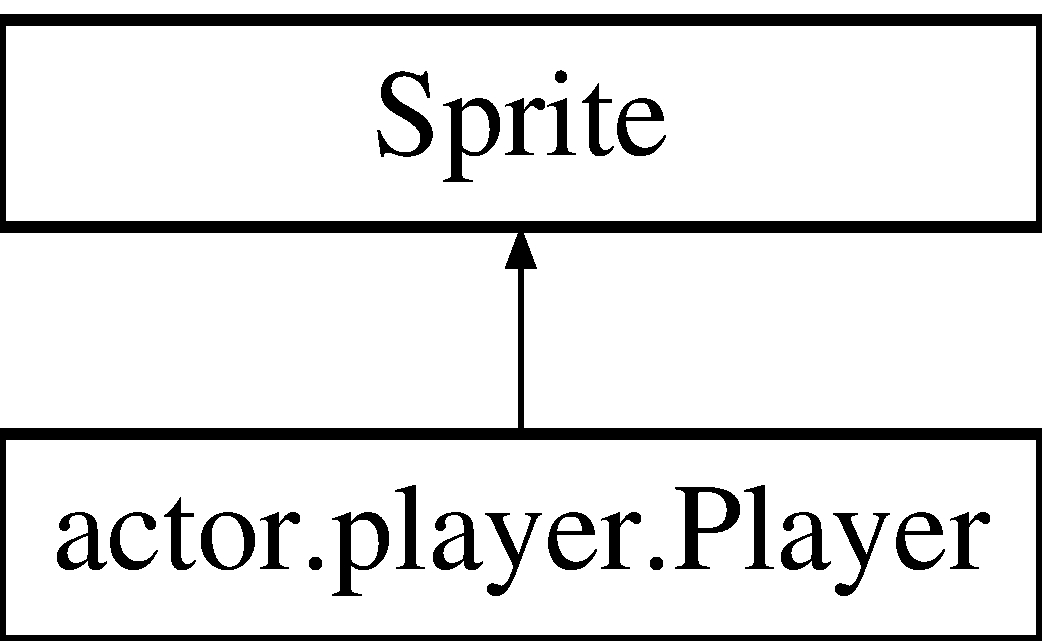
\includegraphics[height=2.000000cm]{classactor_1_1player_1_1_player}
\end{center}
\end{figure}
\subsection*{Public Member Functions}
\begin{DoxyCompactItemize}
\item 
def \hyperlink{classactor_1_1player_1_1_player_ab706da8ac6c2ddecb694069c9c55485b}{\+\_\+\+\_\+init\+\_\+\+\_\+} (self, x, y, hud)
\begin{DoxyCompactList}\small\item\em \hyperlink{classactor_1_1player_1_1_player}{Player} constructor  The constructor for the player object, used within the initialization of the game. \end{DoxyCompactList}\item 
\mbox{\Hypertarget{classactor_1_1player_1_1_player_a43e8f90a1db2286bfb59f80853dcb336}\label{classactor_1_1player_1_1_player_a43e8f90a1db2286bfb59f80853dcb336}} 
def \hyperlink{classactor_1_1player_1_1_player_a43e8f90a1db2286bfb59f80853dcb336}{movechar} (self)
\begin{DoxyCompactList}\small\item\em Function to move the player in a specified direction. \end{DoxyCompactList}\item 
def \hyperlink{classactor_1_1player_1_1_player_a8ac11a22aa47b7febd29d1c740f00452}{move} (self, d, b)
\begin{DoxyCompactList}\small\item\em Function to store which movement buttons are being pressed and let go of by the user. \end{DoxyCompactList}\item 
\mbox{\Hypertarget{classactor_1_1player_1_1_player_a2b481f9bd7f42a0dc98beec777ec5401}\label{classactor_1_1player_1_1_player_a2b481f9bd7f42a0dc98beec777ec5401}} 
def \hyperlink{classactor_1_1player_1_1_player_a2b481f9bd7f42a0dc98beec777ec5401}{attack} (self)
\begin{DoxyCompactList}\small\item\em Function to react to the user pressing the attack button, putting the player into an attack animation and spawning a sword for the duration. \end{DoxyCompactList}\item 
\mbox{\Hypertarget{classactor_1_1player_1_1_player_aacc64de5a021da2b0cfd9535309617e3}\label{classactor_1_1player_1_1_player_aacc64de5a021da2b0cfd9535309617e3}} 
def \hyperlink{classactor_1_1player_1_1_player_aacc64de5a021da2b0cfd9535309617e3}{useitem} (self)
\begin{DoxyCompactList}\small\item\em Function to react to the user pressing the use item button, putting the player into an attack animation and spawning a boomerang for the duration. \end{DoxyCompactList}\item 
def \hyperlink{classactor_1_1player_1_1_player_a709570fc745642d3ad2764e4d973491b}{moveupdate} (self)
\begin{DoxyCompactList}\small\item\em U\+P\+D\+A\+TE L\+O\+OP F\+U\+N\+C\+T\+I\+O\+NS. \end{DoxyCompactList}\item 
def \hyperlink{classactor_1_1player_1_1_player_ab05b71626b99e6cb0babce2d9f7bbb49}{attackupdate} (self)
\begin{DoxyCompactList}\small\item\em Update function for attack and boomerang conditions, as well as handing user collision with enemies (damage taken)  Checks sword collision on enemies, and checks the timeout on both the sword and boomerang attack animations, telling the player when they can move again. \end{DoxyCompactList}\item 
\mbox{\Hypertarget{classactor_1_1player_1_1_player_a427c65b6cb4d5b960493ead3cfc3fda1}\label{classactor_1_1player_1_1_player_a427c65b6cb4d5b960493ead3cfc3fda1}} 
def \hyperlink{classactor_1_1player_1_1_player_a427c65b6cb4d5b960493ead3cfc3fda1}{collisionupdate} (self)
\begin{DoxyCompactList}\small\item\em Update function to check collisions between the player and any specified collidable objects, and call their respective collision events. \end{DoxyCompactList}\item 
\mbox{\Hypertarget{classactor_1_1player_1_1_player_a20c476e0a1df612e3560916b9beda6ef}\label{classactor_1_1player_1_1_player_a20c476e0a1df612e3560916b9beda6ef}} 
def \hyperlink{classactor_1_1player_1_1_player_a20c476e0a1df612e3560916b9beda6ef}{update} (self)
\begin{DoxyCompactList}\small\item\em \hyperlink{classactor_1_1player_1_1_player}{Player} master update function, running all update functions, repeated in main file loop. \end{DoxyCompactList}\end{DoxyCompactItemize}
\subsection*{Public Attributes}
\begin{DoxyCompactItemize}
\item 
\mbox{\Hypertarget{classactor_1_1player_1_1_player_a3f083bf2ff3a0c9fd8838d1292eb6c24}\label{classactor_1_1player_1_1_player_a3f083bf2ff3a0c9fd8838d1292eb6c24}} 
\hyperlink{classactor_1_1player_1_1_player_a3f083bf2ff3a0c9fd8838d1292eb6c24}{image}
\begin{DoxyCompactList}\small\item\em \hyperlink{classactor_1_1player_1_1_player}{Player} sprite image. \end{DoxyCompactList}\item 
\mbox{\Hypertarget{classactor_1_1player_1_1_player_ae166fad5513e8a1afbf28b7090f84385}\label{classactor_1_1player_1_1_player_ae166fad5513e8a1afbf28b7090f84385}} 
\hyperlink{classactor_1_1player_1_1_player_ae166fad5513e8a1afbf28b7090f84385}{id}
\begin{DoxyCompactList}\small\item\em Collision ID (To tell other objects what this object is) \end{DoxyCompactList}\item 
\mbox{\Hypertarget{classactor_1_1player_1_1_player_a80b827225d4cd1ece986735ed50ccaab}\label{classactor_1_1player_1_1_player_a80b827225d4cd1ece986735ed50ccaab}} 
\hyperlink{classactor_1_1player_1_1_player_a80b827225d4cd1ece986735ed50ccaab}{leveltrans}
\begin{DoxyCompactList}\small\item\em Boolean value to tell the game when the player has left the room, and a room transition is needed. \end{DoxyCompactList}\item 
\mbox{\Hypertarget{classactor_1_1player_1_1_player_a17fb13fa8c9bb02af137a6f5e83d2620}\label{classactor_1_1player_1_1_player_a17fb13fa8c9bb02af137a6f5e83d2620}} 
\hyperlink{classactor_1_1player_1_1_player_a17fb13fa8c9bb02af137a6f5e83d2620}{rect}
\begin{DoxyCompactList}\small\item\em \hyperlink{classactor_1_1player_1_1_player}{Player} x and y position. \end{DoxyCompactList}\item 
\mbox{\Hypertarget{classactor_1_1player_1_1_player_a6a324fb53de6ee4b4bab31ea3fc0ffcf}\label{classactor_1_1player_1_1_player_a6a324fb53de6ee4b4bab31ea3fc0ffcf}} 
\hyperlink{classactor_1_1player_1_1_player_a6a324fb53de6ee4b4bab31ea3fc0ffcf}{walk\+Left}
\begin{DoxyCompactList}\small\item\em Animation sprites for player walking left. \end{DoxyCompactList}\item 
\mbox{\Hypertarget{classactor_1_1player_1_1_player_ae4f80d82c8fa045ba5f244d3418b1a1a}\label{classactor_1_1player_1_1_player_ae4f80d82c8fa045ba5f244d3418b1a1a}} 
\hyperlink{classactor_1_1player_1_1_player_ae4f80d82c8fa045ba5f244d3418b1a1a}{walk\+Right}
\begin{DoxyCompactList}\small\item\em Animation sprites for player walking right. \end{DoxyCompactList}\item 
\mbox{\Hypertarget{classactor_1_1player_1_1_player_ae184fcb45669b5da9ce115fcf4446099}\label{classactor_1_1player_1_1_player_ae184fcb45669b5da9ce115fcf4446099}} 
\hyperlink{classactor_1_1player_1_1_player_ae184fcb45669b5da9ce115fcf4446099}{walk\+Up}
\begin{DoxyCompactList}\small\item\em Animation sprites for player walking up. \end{DoxyCompactList}\item 
\mbox{\Hypertarget{classactor_1_1player_1_1_player_a4671e233ca20a575cd6cf6019a56bb12}\label{classactor_1_1player_1_1_player_a4671e233ca20a575cd6cf6019a56bb12}} 
\hyperlink{classactor_1_1player_1_1_player_a4671e233ca20a575cd6cf6019a56bb12}{walk\+Down}
\begin{DoxyCompactList}\small\item\em Animation sprites for player walking down. \end{DoxyCompactList}\item 
\mbox{\Hypertarget{classactor_1_1player_1_1_player_a544178e6ebb1b49a348753c870df24f1}\label{classactor_1_1player_1_1_player_a544178e6ebb1b49a348753c870df24f1}} 
\hyperlink{classactor_1_1player_1_1_player_a544178e6ebb1b49a348753c870df24f1}{attacksprite}
\begin{DoxyCompactList}\small\item\em Animation sprites for player attacking. \end{DoxyCompactList}\item 
\mbox{\Hypertarget{classactor_1_1player_1_1_player_a4f3f92ac7e33ec63e49914610d1cd5ed}\label{classactor_1_1player_1_1_player_a4f3f92ac7e33ec63e49914610d1cd5ed}} 
\hyperlink{classactor_1_1player_1_1_player_a4f3f92ac7e33ec63e49914610d1cd5ed}{obj}
\begin{DoxyCompactList}\small\item\em List of objects that the player can collide with. \end{DoxyCompactList}\item 
\mbox{\Hypertarget{classactor_1_1player_1_1_player_a8678a9b7bbec1f8a257498fdd66597fb}\label{classactor_1_1player_1_1_player_a8678a9b7bbec1f8a257498fdd66597fb}} 
\hyperlink{classactor_1_1player_1_1_player_a8678a9b7bbec1f8a257498fdd66597fb}{hbar}
\begin{DoxyCompactList}\small\item\em Health bar corresponding to the player\textquotesingle{}s health. \end{DoxyCompactList}\item 
\mbox{\Hypertarget{classactor_1_1player_1_1_player_a31f4d4cef26800b302bb683ab0008851}\label{classactor_1_1player_1_1_player_a31f4d4cef26800b302bb683ab0008851}} 
\hyperlink{classactor_1_1player_1_1_player_a31f4d4cef26800b302bb683ab0008851}{rbar}
\begin{DoxyCompactList}\small\item\em Rupee bar corresponding to the player\textquotesingle{}s rupy count. \end{DoxyCompactList}\item 
\mbox{\Hypertarget{classactor_1_1player_1_1_player_afa08d9f1172947ccc9eb5e5bae3a7a8e}\label{classactor_1_1player_1_1_player_afa08d9f1172947ccc9eb5e5bae3a7a8e}} 
\hyperlink{classactor_1_1player_1_1_player_afa08d9f1172947ccc9eb5e5bae3a7a8e}{kbar}
\begin{DoxyCompactList}\small\item\em Key bar corresponding to the player\textquotesingle{}s key count. \end{DoxyCompactList}\item 
\mbox{\Hypertarget{classactor_1_1player_1_1_player_af93fcffe1d5f4b16ad7ca71b54a779d7}\label{classactor_1_1player_1_1_player_af93fcffe1d5f4b16ad7ca71b54a779d7}} 
\hyperlink{classactor_1_1player_1_1_player_af93fcffe1d5f4b16ad7ca71b54a779d7}{totalhp}
\begin{DoxyCompactList}\small\item\em \hyperlink{classactor_1_1player_1_1_player}{Player}\textquotesingle{}s maximum HP amount. \end{DoxyCompactList}\item 
\mbox{\Hypertarget{classactor_1_1player_1_1_player_ae153752032a484c8f84d11a3bd4ad922}\label{classactor_1_1player_1_1_player_ae153752032a484c8f84d11a3bd4ad922}} 
\hyperlink{classactor_1_1player_1_1_player_ae153752032a484c8f84d11a3bd4ad922}{hp}
\begin{DoxyCompactList}\small\item\em \hyperlink{classactor_1_1player_1_1_player}{Player}\textquotesingle{}s current HP amount (starts at max) \end{DoxyCompactList}\item 
\mbox{\Hypertarget{classactor_1_1player_1_1_player_aafe402d4ccb42214e7afa642a97a91ee}\label{classactor_1_1player_1_1_player_aafe402d4ccb42214e7afa642a97a91ee}} 
\hyperlink{classactor_1_1player_1_1_player_aafe402d4ccb42214e7afa642a97a91ee}{rupes}
\begin{DoxyCompactList}\small\item\em \hyperlink{classactor_1_1player_1_1_player}{Player}\textquotesingle{}s rupee counter. \end{DoxyCompactList}\item 
\mbox{\Hypertarget{classactor_1_1player_1_1_player_a2be3c96f039bbc8e535f2bc2a9379b75}\label{classactor_1_1player_1_1_player_a2be3c96f039bbc8e535f2bc2a9379b75}} 
\hyperlink{classactor_1_1player_1_1_player_a2be3c96f039bbc8e535f2bc2a9379b75}{keys}
\begin{DoxyCompactList}\small\item\em \hyperlink{classactor_1_1player_1_1_player}{Player}\textquotesingle{}s key counter. \end{DoxyCompactList}\item 
\mbox{\Hypertarget{classactor_1_1player_1_1_player_a2d44111bc500754466a7cc60f560a3b1}\label{classactor_1_1player_1_1_player_a2d44111bc500754466a7cc60f560a3b1}} 
\hyperlink{classactor_1_1player_1_1_player_a2d44111bc500754466a7cc60f560a3b1}{collision}
\begin{DoxyCompactList}\small\item\em Whether the player is currently colliding with anything. \end{DoxyCompactList}\item 
\mbox{\Hypertarget{classactor_1_1player_1_1_player_ae7fd956a4af73cb7079ebac7fd02c500}\label{classactor_1_1player_1_1_player_ae7fd956a4af73cb7079ebac7fd02c500}} 
\hyperlink{classactor_1_1player_1_1_player_ae7fd956a4af73cb7079ebac7fd02c500}{collidbuy}
\begin{DoxyCompactList}\small\item\em Whether the player has collided with the shop object. \end{DoxyCompactList}\item 
\mbox{\Hypertarget{classactor_1_1player_1_1_player_ad9f2b3abde9b91875f4840fed4f64da2}\label{classactor_1_1player_1_1_player_ad9f2b3abde9b91875f4840fed4f64da2}} 
\hyperlink{classactor_1_1player_1_1_player_ad9f2b3abde9b91875f4840fed4f64da2}{doorcount}
\begin{DoxyCompactList}\small\item\em How long the player needs to walk into a locked door to use a key and unlock it (Prevents touching and unlocking doors by accident) \end{DoxyCompactList}\item 
\mbox{\Hypertarget{classactor_1_1player_1_1_player_ab086494231fe0db5a191209fb496aa32}\label{classactor_1_1player_1_1_player_ab086494231fe0db5a191209fb496aa32}} 
\hyperlink{classactor_1_1player_1_1_player_ab086494231fe0db5a191209fb496aa32}{spawning}
\begin{DoxyCompactList}\small\item\em Checks whether the player has just entered a room. \end{DoxyCompactList}\item 
\mbox{\Hypertarget{classactor_1_1player_1_1_player_acf96b0094e3294d7c0d0dcc23a2450e2}\label{classactor_1_1player_1_1_player_acf96b0094e3294d7c0d0dcc23a2450e2}} 
\hyperlink{classactor_1_1player_1_1_player_acf96b0094e3294d7c0d0dcc23a2450e2}{spawncount}
\begin{DoxyCompactList}\small\item\em Number of frames before the user can take control of the player when they enter a room. \end{DoxyCompactList}\item 
\mbox{\Hypertarget{classactor_1_1player_1_1_player_a62a06e2de507cf924ceb42c478e0acb9}\label{classactor_1_1player_1_1_player_a62a06e2de507cf924ceb42c478e0acb9}} 
\hyperlink{classactor_1_1player_1_1_player_a62a06e2de507cf924ceb42c478e0acb9}{moveable}
\begin{DoxyCompactList}\small\item\em Boolean allowing and stoping the player from moving. \end{DoxyCompactList}\item 
\mbox{\Hypertarget{classactor_1_1player_1_1_player_a77d57d979bab2c2918501b536130cd4f}\label{classactor_1_1player_1_1_player_a77d57d979bab2c2918501b536130cd4f}} 
\hyperlink{classactor_1_1player_1_1_player_a77d57d979bab2c2918501b536130cd4f}{attackbool}
\begin{DoxyCompactList}\small\item\em Boolean to tell whether the player is attacking or not. \end{DoxyCompactList}\item 
\mbox{\Hypertarget{classactor_1_1player_1_1_player_a9014fc320d75f42a42067131ef359521}\label{classactor_1_1player_1_1_player_a9014fc320d75f42a42067131ef359521}} 
\hyperlink{classactor_1_1player_1_1_player_a9014fc320d75f42a42067131ef359521}{attackcount}
\begin{DoxyCompactList}\small\item\em Attack counter, to control how long the attack lasts. \end{DoxyCompactList}\item 
\hyperlink{classactor_1_1player_1_1_player_a479ddb8958705d9cbd7830e9ba59f8c5}{attacksword}
\begin{DoxyCompactList}\small\item\em Holder for a sword object when attacking. \end{DoxyCompactList}\item 
\mbox{\Hypertarget{classactor_1_1player_1_1_player_a6c97e5519cba645d52374ef46537b913}\label{classactor_1_1player_1_1_player_a6c97e5519cba645d52374ef46537b913}} 
\hyperlink{classactor_1_1player_1_1_player_a6c97e5519cba645d52374ef46537b913}{item}
\begin{DoxyCompactList}\small\item\em Holder for a boomerang object when using item. \end{DoxyCompactList}\item 
\mbox{\Hypertarget{classactor_1_1player_1_1_player_ad03534ba44251c9d8d6b72d2b1cc027e}\label{classactor_1_1player_1_1_player_ad03534ba44251c9d8d6b72d2b1cc027e}} 
\hyperlink{classactor_1_1player_1_1_player_ad03534ba44251c9d8d6b72d2b1cc027e}{itembool}
\begin{DoxyCompactList}\small\item\em Boolean to tell whether the player is using their boomerang or not. \end{DoxyCompactList}\item 
\mbox{\Hypertarget{classactor_1_1player_1_1_player_a1dd72a6eb3f660ee7ae95848e534b5b4}\label{classactor_1_1player_1_1_player_a1dd72a6eb3f660ee7ae95848e534b5b4}} 
\hyperlink{classactor_1_1player_1_1_player_a1dd72a6eb3f660ee7ae95848e534b5b4}{oldx}
\begin{DoxyCompactList}\small\item\em \hyperlink{classactor_1_1player_1_1_player}{Player}\textquotesingle{}s x value one frame ago. \end{DoxyCompactList}\item 
\mbox{\Hypertarget{classactor_1_1player_1_1_player_a732ab21f88b48cad06541e86e4f5166c}\label{classactor_1_1player_1_1_player_a732ab21f88b48cad06541e86e4f5166c}} 
\hyperlink{classactor_1_1player_1_1_player_a732ab21f88b48cad06541e86e4f5166c}{oldy}
\begin{DoxyCompactList}\small\item\em \hyperlink{classactor_1_1player_1_1_player}{Player}\textquotesingle{}s y value one frame ago. \end{DoxyCompactList}\item 
\mbox{\Hypertarget{classactor_1_1player_1_1_player_aae66aa3ba8ee37f20c3f24278c203f5b}\label{classactor_1_1player_1_1_player_aae66aa3ba8ee37f20c3f24278c203f5b}} 
\hyperlink{classactor_1_1player_1_1_player_aae66aa3ba8ee37f20c3f24278c203f5b}{dirbool}
\begin{DoxyCompactList}\small\item\em Boolean array to tell which directional buttons are pressed or not (starting left going clockwise, dirbool\mbox{[}0\mbox{]} is left, dirbool\mbox{[}1\mbox{]} is up, etc) \end{DoxyCompactList}\item 
\hyperlink{classactor_1_1player_1_1_player_a569ec214c309ddbf82e414c310861832}{dir}
\begin{DoxyCompactList}\small\item\em Current direction the player is facing. \end{DoxyCompactList}\item 
\mbox{\Hypertarget{classactor_1_1player_1_1_player_a80a7403771d9fb980354b43241eb21d2}\label{classactor_1_1player_1_1_player_a80a7403771d9fb980354b43241eb21d2}} 
\hyperlink{classactor_1_1player_1_1_player_a80a7403771d9fb980354b43241eb21d2}{hit}
\begin{DoxyCompactList}\small\item\em Boolean on whether the player was recently hit. \end{DoxyCompactList}\item 
\mbox{\Hypertarget{classactor_1_1player_1_1_player_a0c6434fb932d898b1ec1ed77c97d46b5}\label{classactor_1_1player_1_1_player_a0c6434fb932d898b1ec1ed77c97d46b5}} 
\hyperlink{classactor_1_1player_1_1_player_a0c6434fb932d898b1ec1ed77c97d46b5}{hitcount}
\begin{DoxyCompactList}\small\item\em How long a hit counts for on the player (how long until self.\+hit turns off) \end{DoxyCompactList}\item 
\mbox{\Hypertarget{classactor_1_1player_1_1_player_a303bd9cebacff3d0c25b359e18d7bb3a}\label{classactor_1_1player_1_1_player_a303bd9cebacff3d0c25b359e18d7bb3a}} 
\hyperlink{classactor_1_1player_1_1_player_a303bd9cebacff3d0c25b359e18d7bb3a}{speed}
\begin{DoxyCompactList}\small\item\em Per-\/frame unit speed of player. \end{DoxyCompactList}\item 
\mbox{\Hypertarget{classactor_1_1player_1_1_player_a5cf8c2343817f5fdf357579fc078b677}\label{classactor_1_1player_1_1_player_a5cf8c2343817f5fdf357579fc078b677}} 
\hyperlink{classactor_1_1player_1_1_player_a5cf8c2343817f5fdf357579fc078b677}{debug}
\begin{DoxyCompactList}\small\item\em Whether debug mode is on/off. \end{DoxyCompactList}\item 
\mbox{\Hypertarget{classactor_1_1player_1_1_player_aa3b90c5623839511cd22f4e0ee1745ea}\label{classactor_1_1player_1_1_player_aa3b90c5623839511cd22f4e0ee1745ea}} 
\hyperlink{classactor_1_1player_1_1_player_aa3b90c5623839511cd22f4e0ee1745ea}{has\+Won}
\begin{DoxyCompactList}\small\item\em Has the player won or not. \end{DoxyCompactList}\end{DoxyCompactItemize}


\subsection{Detailed Description}
\hyperlink{classactor_1_1player_1_1_player}{Player} Class  A pygame sprite subclass for defining the creation of the game\textquotesingle{}s playable character, as well as its interactions with both the user and other entities within the game. 

\subsection{Constructor \& Destructor Documentation}
\mbox{\Hypertarget{classactor_1_1player_1_1_player_ab706da8ac6c2ddecb694069c9c55485b}\label{classactor_1_1player_1_1_player_ab706da8ac6c2ddecb694069c9c55485b}} 
\index{actor\+::player\+::\+Player@{actor\+::player\+::\+Player}!\+\_\+\+\_\+init\+\_\+\+\_\+@{\+\_\+\+\_\+init\+\_\+\+\_\+}}
\index{\+\_\+\+\_\+init\+\_\+\+\_\+@{\+\_\+\+\_\+init\+\_\+\+\_\+}!actor\+::player\+::\+Player@{actor\+::player\+::\+Player}}
\subsubsection{\texorpdfstring{\+\_\+\+\_\+init\+\_\+\+\_\+()}{\_\_init\_\_()}}
{\footnotesize\ttfamily def actor.\+player.\+Player.\+\_\+\+\_\+init\+\_\+\+\_\+ (\begin{DoxyParamCaption}\item[{}]{self,  }\item[{}]{x,  }\item[{}]{y,  }\item[{}]{hud }\end{DoxyParamCaption})}



\hyperlink{classactor_1_1player_1_1_player}{Player} constructor  The constructor for the player object, used within the initialization of the game. 

The only arguments passed are an initial x and y position, as well as heads-\/up-\/display (H\+UD) elements. 
\begin{DoxyParams}{Parameters}
{\em x} & Initial player x coordinate \\
\hline
{\em y} & Initial player y coordinate \\
\hline
{\em hud} & Array of H\+UD elements which act directly with the user\textquotesingle{}s tracked values (health bar, rupy/key count) \\
\hline
\end{DoxyParams}


\subsection{Member Function Documentation}
\mbox{\Hypertarget{classactor_1_1player_1_1_player_ab05b71626b99e6cb0babce2d9f7bbb49}\label{classactor_1_1player_1_1_player_ab05b71626b99e6cb0babce2d9f7bbb49}} 
\index{actor\+::player\+::\+Player@{actor\+::player\+::\+Player}!attackupdate@{attackupdate}}
\index{attackupdate@{attackupdate}!actor\+::player\+::\+Player@{actor\+::player\+::\+Player}}
\subsubsection{\texorpdfstring{attackupdate()}{attackupdate()}}
{\footnotesize\ttfamily def actor.\+player.\+Player.\+attackupdate (\begin{DoxyParamCaption}\item[{}]{self }\end{DoxyParamCaption})}



Update function for attack and boomerang conditions, as well as handing user collision with enemies (damage taken)  Checks sword collision on enemies, and checks the timeout on both the sword and boomerang attack animations, telling the player when they can move again. 

Also updates the player and reacts accordingly to recieving damage. \mbox{\Hypertarget{classactor_1_1player_1_1_player_a8ac11a22aa47b7febd29d1c740f00452}\label{classactor_1_1player_1_1_player_a8ac11a22aa47b7febd29d1c740f00452}} 
\index{actor\+::player\+::\+Player@{actor\+::player\+::\+Player}!move@{move}}
\index{move@{move}!actor\+::player\+::\+Player@{actor\+::player\+::\+Player}}
\subsubsection{\texorpdfstring{move()}{move()}}
{\footnotesize\ttfamily def actor.\+player.\+Player.\+move (\begin{DoxyParamCaption}\item[{}]{self,  }\item[{}]{d,  }\item[{}]{b }\end{DoxyParamCaption})}



Function to store which movement buttons are being pressed and let go of by the user. 


\begin{DoxyParams}{Parameters}
{\em d} & Direction related to the button pressed (integer value from 0 to 3, starting from the left and going clockwise) \\
\hline
{\em b} & Boolean value on whether the button is pressed or not \\
\hline
\end{DoxyParams}
\mbox{\Hypertarget{classactor_1_1player_1_1_player_a709570fc745642d3ad2764e4d973491b}\label{classactor_1_1player_1_1_player_a709570fc745642d3ad2764e4d973491b}} 
\index{actor\+::player\+::\+Player@{actor\+::player\+::\+Player}!moveupdate@{moveupdate}}
\index{moveupdate@{moveupdate}!actor\+::player\+::\+Player@{actor\+::player\+::\+Player}}
\subsubsection{\texorpdfstring{moveupdate()}{moveupdate()}}
{\footnotesize\ttfamily def actor.\+player.\+Player.\+moveupdate (\begin{DoxyParamCaption}\item[{}]{self }\end{DoxyParamCaption})}



U\+P\+D\+A\+TE L\+O\+OP F\+U\+N\+C\+T\+I\+O\+NS. 

Update function for player movement and according sprite animation 

\subsection{Member Data Documentation}
\mbox{\Hypertarget{classactor_1_1player_1_1_player_a479ddb8958705d9cbd7830e9ba59f8c5}\label{classactor_1_1player_1_1_player_a479ddb8958705d9cbd7830e9ba59f8c5}} 
\index{actor\+::player\+::\+Player@{actor\+::player\+::\+Player}!attacksword@{attacksword}}
\index{attacksword@{attacksword}!actor\+::player\+::\+Player@{actor\+::player\+::\+Player}}
\subsubsection{\texorpdfstring{attacksword}{attacksword}}
{\footnotesize\ttfamily actor.\+player.\+Player.\+attacksword}



Holder for a sword object when attacking. 

Sprite function to delete a sprite object and all relations of the object in the project. \mbox{\Hypertarget{classactor_1_1player_1_1_player_a569ec214c309ddbf82e414c310861832}\label{classactor_1_1player_1_1_player_a569ec214c309ddbf82e414c310861832}} 
\index{actor\+::player\+::\+Player@{actor\+::player\+::\+Player}!dir@{dir}}
\index{dir@{dir}!actor\+::player\+::\+Player@{actor\+::player\+::\+Player}}
\subsubsection{\texorpdfstring{dir}{dir}}
{\footnotesize\ttfamily actor.\+player.\+Player.\+dir}



Current direction the player is facing. 

Render Appropriate Sprites According to movement. 

The documentation for this class was generated from the following file\+:\begin{DoxyCompactItemize}
\item 
src/actor/\hyperlink{player_8py}{player.\+py}\end{DoxyCompactItemize}

\hypertarget{classactor_1_1rupee_1_1_rupee___bar}{}\section{actor.\+rupee.\+Rupee\+\_\+\+Bar Class Reference}
\label{classactor_1_1rupee_1_1_rupee___bar}\index{actor.\+rupee.\+Rupee\+\_\+\+Bar@{actor.\+rupee.\+Rupee\+\_\+\+Bar}}


This class represents the Rupee\+Bar object.  


Inheritance diagram for actor.\+rupee.\+Rupee\+\_\+\+Bar\+:\begin{figure}[H]
\begin{center}
\leavevmode
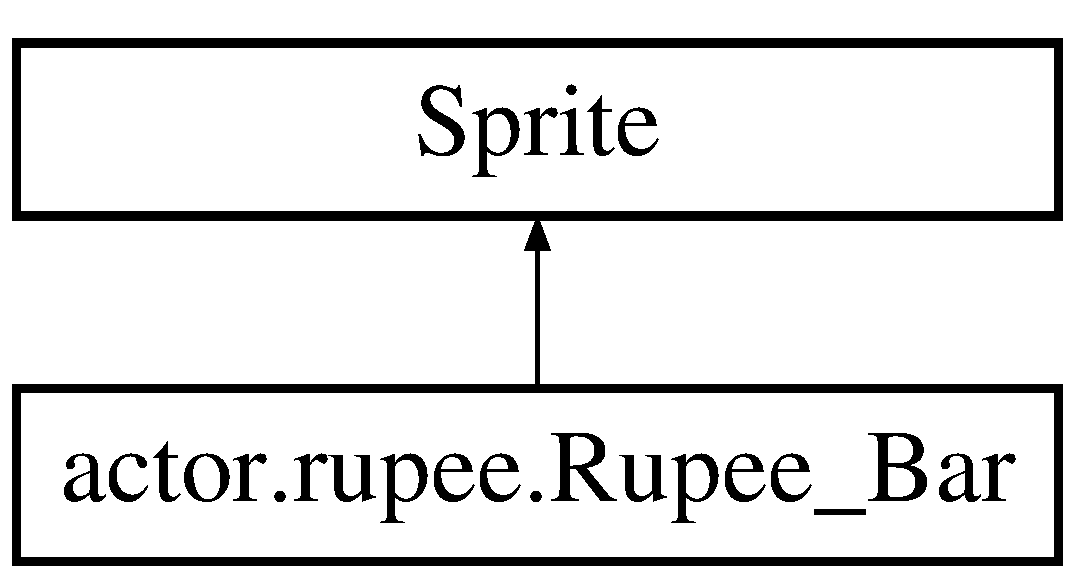
\includegraphics[height=2.000000cm]{classactor_1_1rupee_1_1_rupee___bar}
\end{center}
\end{figure}
\subsection*{Public Member Functions}
\begin{DoxyCompactItemize}
\item 
def \hyperlink{classactor_1_1rupee_1_1_rupee___bar_acd0085452fdaff7478db209487bc8a80}{\+\_\+\+\_\+init\+\_\+\+\_\+} (self, x, y)
\begin{DoxyCompactList}\small\item\em Constructor for the Rupee\+Bar object. \end{DoxyCompactList}\end{DoxyCompactItemize}
\subsection*{Public Attributes}
\begin{DoxyCompactItemize}
\item 
\hyperlink{classactor_1_1rupee_1_1_rupee___bar_a8a0f7e6f0ac2c12e172d691e2fe4aba4}{image}
\begin{DoxyCompactList}\small\item\em This represents the sprite image of the \hyperlink{classactor_1_1rupee_1_1_rupee___bar}{Rupee\+\_\+\+Bar} object. \end{DoxyCompactList}\item 
\hyperlink{classactor_1_1rupee_1_1_rupee___bar_ace89c66353c7b26fafa8a52a5fec2733}{rect}
\begin{DoxyCompactList}\small\item\em This represents rectangle for collision and position for the sprite image of the \hyperlink{classactor_1_1rupee_1_1_rupee___bar}{Rupee\+\_\+\+Bar} object. \end{DoxyCompactList}\end{DoxyCompactItemize}


\subsection{Detailed Description}
This class represents the Rupee\+Bar object. 

The Rupee class uses the Pygame library and Sprite\+Sheet module to create an image for the 

\subsection{Constructor \& Destructor Documentation}
\mbox{\Hypertarget{classactor_1_1rupee_1_1_rupee___bar_acd0085452fdaff7478db209487bc8a80}\label{classactor_1_1rupee_1_1_rupee___bar_acd0085452fdaff7478db209487bc8a80}} 
\index{actor\+::rupee\+::\+Rupee\+\_\+\+Bar@{actor\+::rupee\+::\+Rupee\+\_\+\+Bar}!\+\_\+\+\_\+init\+\_\+\+\_\+@{\+\_\+\+\_\+init\+\_\+\+\_\+}}
\index{\+\_\+\+\_\+init\+\_\+\+\_\+@{\+\_\+\+\_\+init\+\_\+\+\_\+}!actor\+::rupee\+::\+Rupee\+\_\+\+Bar@{actor\+::rupee\+::\+Rupee\+\_\+\+Bar}}
\subsubsection{\texorpdfstring{\+\_\+\+\_\+init\+\_\+\+\_\+()}{\_\_init\_\_()}}
{\footnotesize\ttfamily def actor.\+rupee.\+Rupee\+\_\+\+Bar.\+\_\+\+\_\+init\+\_\+\+\_\+ (\begin{DoxyParamCaption}\item[{}]{self,  }\item[{}]{x,  }\item[{}]{y }\end{DoxyParamCaption})}



Constructor for the Rupee\+Bar object. 

Constructor for class initializes the x and y location of the Rupee\+Bar object. 
\begin{DoxyParams}{Parameters}
{\em x} & this represents the x-\/coordinate at which the Rupee\+Bar object will be drawn. \\
\hline
{\em y} & this represents the y-\/coordinate at which the Rupeeh\+Bar object will be drawn. \\
\hline
\end{DoxyParams}


\subsection{Member Data Documentation}
\mbox{\Hypertarget{classactor_1_1rupee_1_1_rupee___bar_a8a0f7e6f0ac2c12e172d691e2fe4aba4}\label{classactor_1_1rupee_1_1_rupee___bar_a8a0f7e6f0ac2c12e172d691e2fe4aba4}} 
\index{actor\+::rupee\+::\+Rupee\+\_\+\+Bar@{actor\+::rupee\+::\+Rupee\+\_\+\+Bar}!image@{image}}
\index{image@{image}!actor\+::rupee\+::\+Rupee\+\_\+\+Bar@{actor\+::rupee\+::\+Rupee\+\_\+\+Bar}}
\subsubsection{\texorpdfstring{image}{image}}
{\footnotesize\ttfamily actor.\+rupee.\+Rupee\+\_\+\+Bar.\+image}



This represents the sprite image of the \hyperlink{classactor_1_1rupee_1_1_rupee___bar}{Rupee\+\_\+\+Bar} object. 

\mbox{\Hypertarget{classactor_1_1rupee_1_1_rupee___bar_ace89c66353c7b26fafa8a52a5fec2733}\label{classactor_1_1rupee_1_1_rupee___bar_ace89c66353c7b26fafa8a52a5fec2733}} 
\index{actor\+::rupee\+::\+Rupee\+\_\+\+Bar@{actor\+::rupee\+::\+Rupee\+\_\+\+Bar}!rect@{rect}}
\index{rect@{rect}!actor\+::rupee\+::\+Rupee\+\_\+\+Bar@{actor\+::rupee\+::\+Rupee\+\_\+\+Bar}}
\subsubsection{\texorpdfstring{rect}{rect}}
{\footnotesize\ttfamily actor.\+rupee.\+Rupee\+\_\+\+Bar.\+rect}



This represents rectangle for collision and position for the sprite image of the \hyperlink{classactor_1_1rupee_1_1_rupee___bar}{Rupee\+\_\+\+Bar} object. 



The documentation for this class was generated from the following file\+:\begin{DoxyCompactItemize}
\item 
src/actor/\hyperlink{rupee_8py}{rupee.\+py}\end{DoxyCompactItemize}

\hypertarget{classactor_1_1spritesheet_1_1_sprite_sheet}{}\section{actor.\+spritesheet.\+Sprite\+Sheet Class Reference}
\label{classactor_1_1spritesheet_1_1_sprite_sheet}\index{actor.\+spritesheet.\+Sprite\+Sheet@{actor.\+spritesheet.\+Sprite\+Sheet}}


This class represents the \hyperlink{classactor_1_1spritesheet_1_1_sprite_sheet}{Sprite\+Sheet} object, allowing sprites to be loaded and processed.  


Inheritance diagram for actor.\+spritesheet.\+Sprite\+Sheet\+:\begin{figure}[H]
\begin{center}
\leavevmode
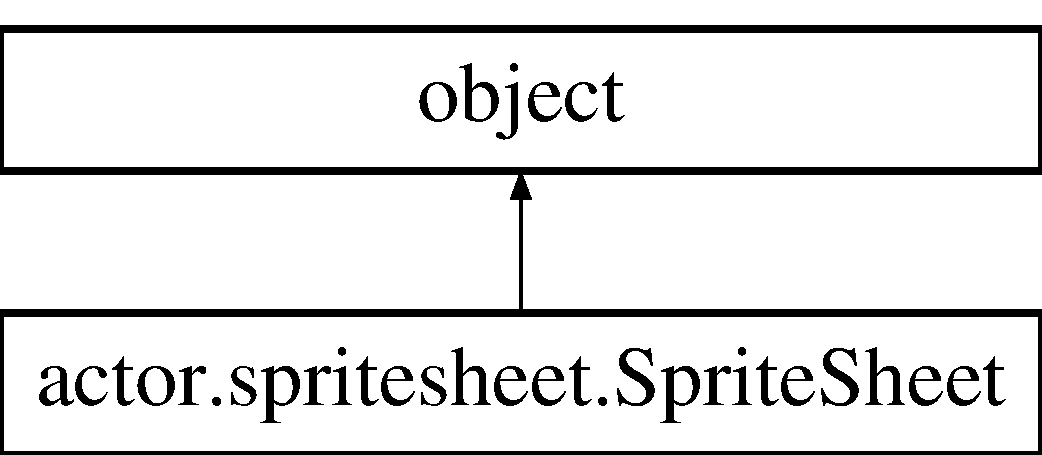
\includegraphics[height=2.000000cm]{classactor_1_1spritesheet_1_1_sprite_sheet}
\end{center}
\end{figure}
\subsection*{Public Member Functions}
\begin{DoxyCompactItemize}
\item 
def \hyperlink{classactor_1_1spritesheet_1_1_sprite_sheet_a00df0cb80c019436add7a699a83c5ae2}{\+\_\+\+\_\+init\+\_\+\+\_\+} (self, file\+\_\+name)
\begin{DoxyCompactList}\small\item\em Constructor for the \hyperlink{classactor_1_1spritesheet_1_1_sprite_sheet}{Sprite\+Sheet} class. \end{DoxyCompactList}\item 
def \hyperlink{classactor_1_1spritesheet_1_1_sprite_sheet_ad2c4f5b00c63a9377b64fe28ef26587b}{get\+\_\+image} (self, x, y, width, height)
\begin{DoxyCompactList}\small\item\em Accessor to return an image splice from the loaded \hyperlink{classactor_1_1spritesheet_1_1_sprite_sheet}{Sprite\+Sheet}. \end{DoxyCompactList}\item 
def \hyperlink{classactor_1_1spritesheet_1_1_sprite_sheet_a2d0883c80dad8344520f40f6fd2b79a6}{get\+\_\+image\+NT} (self, x, y, width, height)
\begin{DoxyCompactList}\small\item\em Accessor to return an image splice from the loaded \hyperlink{classactor_1_1spritesheet_1_1_sprite_sheet}{Sprite\+Sheet}, W\+I\+T\+H\+O\+UT removing the image background. \end{DoxyCompactList}\end{DoxyCompactItemize}
\subsection*{Public Attributes}
\begin{DoxyCompactItemize}
\item 
\hyperlink{classactor_1_1spritesheet_1_1_sprite_sheet_ae4eb015142736df995f9564c47f4ddd6}{sprite\+\_\+sheet}
\begin{DoxyCompactList}\small\item\em This represents the current spritesheet loaded from the specific file\+\_\+name path. \end{DoxyCompactList}\end{DoxyCompactItemize}


\subsection{Detailed Description}
This class represents the \hyperlink{classactor_1_1spritesheet_1_1_sprite_sheet}{Sprite\+Sheet} object, allowing sprites to be loaded and processed. 

The \hyperlink{classactor_1_1spritesheet_1_1_sprite_sheet}{Sprite\+Sheet} class uses the Pygame library to load images and change the transperancy on those images. 

\subsection{Constructor \& Destructor Documentation}
\mbox{\Hypertarget{classactor_1_1spritesheet_1_1_sprite_sheet_a00df0cb80c019436add7a699a83c5ae2}\label{classactor_1_1spritesheet_1_1_sprite_sheet_a00df0cb80c019436add7a699a83c5ae2}} 
\index{actor\+::spritesheet\+::\+Sprite\+Sheet@{actor\+::spritesheet\+::\+Sprite\+Sheet}!\+\_\+\+\_\+init\+\_\+\+\_\+@{\+\_\+\+\_\+init\+\_\+\+\_\+}}
\index{\+\_\+\+\_\+init\+\_\+\+\_\+@{\+\_\+\+\_\+init\+\_\+\+\_\+}!actor\+::spritesheet\+::\+Sprite\+Sheet@{actor\+::spritesheet\+::\+Sprite\+Sheet}}
\subsubsection{\texorpdfstring{\+\_\+\+\_\+init\+\_\+\+\_\+()}{\_\_init\_\_()}}
{\footnotesize\ttfamily def actor.\+spritesheet.\+Sprite\+Sheet.\+\_\+\+\_\+init\+\_\+\+\_\+ (\begin{DoxyParamCaption}\item[{}]{self,  }\item[{}]{file\+\_\+name }\end{DoxyParamCaption})}



Constructor for the \hyperlink{classactor_1_1spritesheet_1_1_sprite_sheet}{Sprite\+Sheet} class. 

This constructor initializes an image file using the Pygame library. 
\begin{DoxyParams}{Parameters}
{\em file\+\_\+name} & This is the string representing the path to the image file. \\
\hline
\end{DoxyParams}


\subsection{Member Function Documentation}
\mbox{\Hypertarget{classactor_1_1spritesheet_1_1_sprite_sheet_ad2c4f5b00c63a9377b64fe28ef26587b}\label{classactor_1_1spritesheet_1_1_sprite_sheet_ad2c4f5b00c63a9377b64fe28ef26587b}} 
\index{actor\+::spritesheet\+::\+Sprite\+Sheet@{actor\+::spritesheet\+::\+Sprite\+Sheet}!get\+\_\+image@{get\+\_\+image}}
\index{get\+\_\+image@{get\+\_\+image}!actor\+::spritesheet\+::\+Sprite\+Sheet@{actor\+::spritesheet\+::\+Sprite\+Sheet}}
\subsubsection{\texorpdfstring{get\+\_\+image()}{get\_image()}}
{\footnotesize\ttfamily def actor.\+spritesheet.\+Sprite\+Sheet.\+get\+\_\+image (\begin{DoxyParamCaption}\item[{}]{self,  }\item[{}]{x,  }\item[{}]{y,  }\item[{}]{width,  }\item[{}]{height }\end{DoxyParamCaption})}



Accessor to return an image splice from the loaded \hyperlink{classactor_1_1spritesheet_1_1_sprite_sheet}{Sprite\+Sheet}. 

This accessor returns an image splice based on the x,y location and the height and width of the image. 
\begin{DoxyParams}{Parameters}
{\em x} & The x-\/coordinate for starting point of the splice on the \hyperlink{classactor_1_1spritesheet_1_1_sprite_sheet}{Sprite\+Sheet}. \\
\hline
{\em y} & The y-\/coordinate for starting point of the splice on the \hyperlink{classactor_1_1spritesheet_1_1_sprite_sheet}{Sprite\+Sheet}. \\
\hline
{\em width} & The width of the splice on the \hyperlink{classactor_1_1spritesheet_1_1_sprite_sheet}{Sprite\+Sheet}. \\
\hline
{\em height} & The height of the splice on the \hyperlink{classactor_1_1spritesheet_1_1_sprite_sheet}{Sprite\+Sheet}. \\
\hline
\end{DoxyParams}
\begin{DoxyReturn}{Returns}
image This returns the newly spliced image after removing the image background transparency. 
\end{DoxyReturn}
\mbox{\Hypertarget{classactor_1_1spritesheet_1_1_sprite_sheet_a2d0883c80dad8344520f40f6fd2b79a6}\label{classactor_1_1spritesheet_1_1_sprite_sheet_a2d0883c80dad8344520f40f6fd2b79a6}} 
\index{actor\+::spritesheet\+::\+Sprite\+Sheet@{actor\+::spritesheet\+::\+Sprite\+Sheet}!get\+\_\+image\+NT@{get\+\_\+image\+NT}}
\index{get\+\_\+image\+NT@{get\+\_\+image\+NT}!actor\+::spritesheet\+::\+Sprite\+Sheet@{actor\+::spritesheet\+::\+Sprite\+Sheet}}
\subsubsection{\texorpdfstring{get\+\_\+image\+N\+T()}{get\_imageNT()}}
{\footnotesize\ttfamily def actor.\+spritesheet.\+Sprite\+Sheet.\+get\+\_\+image\+NT (\begin{DoxyParamCaption}\item[{}]{self,  }\item[{}]{x,  }\item[{}]{y,  }\item[{}]{width,  }\item[{}]{height }\end{DoxyParamCaption})}



Accessor to return an image splice from the loaded \hyperlink{classactor_1_1spritesheet_1_1_sprite_sheet}{Sprite\+Sheet}, W\+I\+T\+H\+O\+UT removing the image background. 

This accessor returns an image splice based on the x,y location and the height and width of the image. 
\begin{DoxyParams}{Parameters}
{\em x} & The x-\/coordinate for starting point of the splice on the \hyperlink{classactor_1_1spritesheet_1_1_sprite_sheet}{Sprite\+Sheet}. \\
\hline
{\em y} & The y-\/coordinate for starting point of the splice on the \hyperlink{classactor_1_1spritesheet_1_1_sprite_sheet}{Sprite\+Sheet}. \\
\hline
{\em width} & The width of the splice on the \hyperlink{classactor_1_1spritesheet_1_1_sprite_sheet}{Sprite\+Sheet}. \\
\hline
{\em height} & The height of the splice on the \hyperlink{classactor_1_1spritesheet_1_1_sprite_sheet}{Sprite\+Sheet}. \\
\hline
\end{DoxyParams}
\begin{DoxyReturn}{Returns}
image This returns the newly spliced image W\+I\+T\+H\+O\+UT removing the image background transparency. 
\end{DoxyReturn}


\subsection{Member Data Documentation}
\mbox{\Hypertarget{classactor_1_1spritesheet_1_1_sprite_sheet_ae4eb015142736df995f9564c47f4ddd6}\label{classactor_1_1spritesheet_1_1_sprite_sheet_ae4eb015142736df995f9564c47f4ddd6}} 
\index{actor\+::spritesheet\+::\+Sprite\+Sheet@{actor\+::spritesheet\+::\+Sprite\+Sheet}!sprite\+\_\+sheet@{sprite\+\_\+sheet}}
\index{sprite\+\_\+sheet@{sprite\+\_\+sheet}!actor\+::spritesheet\+::\+Sprite\+Sheet@{actor\+::spritesheet\+::\+Sprite\+Sheet}}
\subsubsection{\texorpdfstring{sprite\+\_\+sheet}{sprite\_sheet}}
{\footnotesize\ttfamily actor.\+spritesheet.\+Sprite\+Sheet.\+sprite\+\_\+sheet}



This represents the current spritesheet loaded from the specific file\+\_\+name path. 



The documentation for this class was generated from the following file\+:\begin{DoxyCompactItemize}
\item 
src/actor/\hyperlink{spritesheet_8py}{spritesheet.\+py}\end{DoxyCompactItemize}

\hypertarget{classactor_1_1stalfos_1_1_stalfos}{}\section{actor.\+stalfos.\+Stalfos Class Reference}
\label{classactor_1_1stalfos_1_1_stalfos}\index{actor.\+stalfos.\+Stalfos@{actor.\+stalfos.\+Stalfos}}


This class represents the \hyperlink{classactor_1_1stalfos_1_1_stalfos}{Stalfos} enemy.  


Inheritance diagram for actor.\+stalfos.\+Stalfos\+:\begin{figure}[H]
\begin{center}
\leavevmode
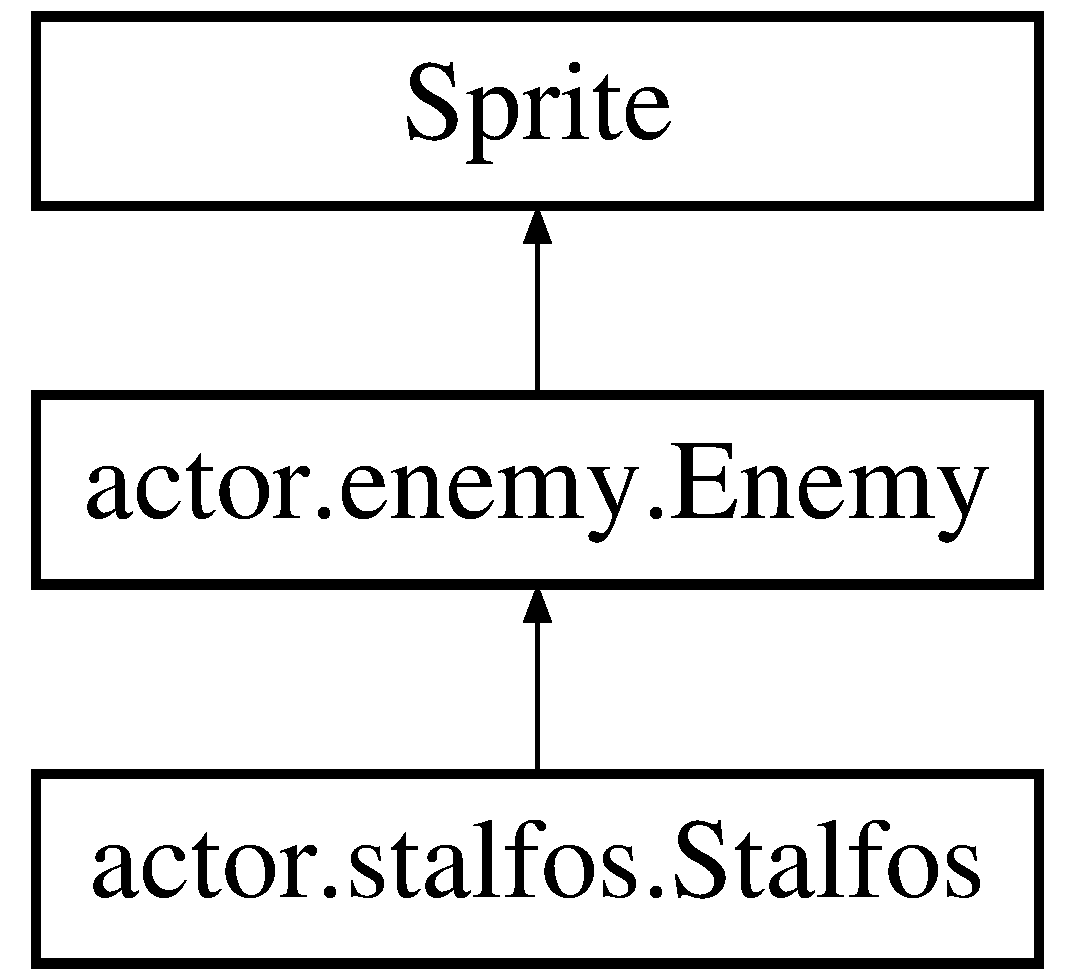
\includegraphics[height=3.000000cm]{classactor_1_1stalfos_1_1_stalfos}
\end{center}
\end{figure}
\subsection*{Public Member Functions}
\begin{DoxyCompactItemize}
\item 
def \hyperlink{classactor_1_1stalfos_1_1_stalfos_ad8c4e62f51605d1b83c80e21263334af}{\+\_\+\+\_\+init\+\_\+\+\_\+} (self, x, y)
\begin{DoxyCompactList}\small\item\em Constructor for \hyperlink{classactor_1_1stalfos_1_1_stalfos}{Stalfos}. \end{DoxyCompactList}\item 
def \hyperlink{classactor_1_1stalfos_1_1_stalfos_adea3ec3198efffc7015efb4b49a44a69}{check\+State} (self)
\begin{DoxyCompactList}\small\item\em Evaluates the state of the \hyperlink{classactor_1_1stalfos_1_1_stalfos}{Stalfos}. \end{DoxyCompactList}\item 
def \hyperlink{classactor_1_1stalfos_1_1_stalfos_a1789c1afbf23d5983dec9432578fd058}{enemy\+Logic} (self)
\begin{DoxyCompactList}\small\item\em Controls \hyperlink{classactor_1_1stalfos_1_1_stalfos}{Stalfos} logic. \end{DoxyCompactList}\item 
def \hyperlink{classactor_1_1stalfos_1_1_stalfos_aba32f6c73afde82b410eee05e86c6545}{gen\+Travel\+Path} (self)
\begin{DoxyCompactList}\small\item\em Creates a new travel point for \hyperlink{classactor_1_1stalfos_1_1_stalfos}{Stalfos}. \end{DoxyCompactList}\item 
def \hyperlink{classactor_1_1stalfos_1_1_stalfos_ac3fe6cc13509504318f492473795dc41}{set\+Walk\+Speed} (self)
\begin{DoxyCompactList}\small\item\em Sets the walk speed of the \hyperlink{classactor_1_1stalfos_1_1_stalfos}{Stalfos}. \end{DoxyCompactList}\item 
def \hyperlink{classactor_1_1stalfos_1_1_stalfos_abb5c74f32bbfa0a9d7d4bfaa60b6f2d7}{stop} (self)
\begin{DoxyCompactList}\small\item\em Stops the \hyperlink{classactor_1_1stalfos_1_1_stalfos}{Stalfos}. \end{DoxyCompactList}\end{DoxyCompactItemize}
\subsection*{Public Attributes}
\begin{DoxyCompactItemize}
\item 
\hyperlink{classactor_1_1stalfos_1_1_stalfos_a75c99c163e71b951ea617a47e2ed1dda}{is\+Moving}
\begin{DoxyCompactList}\small\item\em Call superclass constructor. \end{DoxyCompactList}\item 
\hyperlink{classactor_1_1stalfos_1_1_stalfos_a7e91c289f586728284c20c3963b86b06}{previous\+Direction}
\begin{DoxyCompactList}\small\item\em Movement integer value for previous direction of movement for \hyperlink{classactor_1_1stalfos_1_1_stalfos}{Stalfos} state. \end{DoxyCompactList}\item 
\hyperlink{classactor_1_1stalfos_1_1_stalfos_ae98d09367d88672074d0ae4622b03eda}{direction}
\begin{DoxyCompactList}\small\item\em Movement integer value for current direction of movement for \hyperlink{classactor_1_1stalfos_1_1_stalfos}{Stalfos} state. \end{DoxyCompactList}\item 
\hyperlink{classactor_1_1stalfos_1_1_stalfos_ae583478be5ec05f00f4f3fb460516012}{walk\+Frames}
\begin{DoxyCompactList}\small\item\em Integer representing the frames walked by Staflos in movement state. \end{DoxyCompactList}\item 
\hyperlink{classactor_1_1stalfos_1_1_stalfos_ac0fcfca44d7cc2642a4116806bb6b1b6}{walk\+Start\+Frame}
\begin{DoxyCompactList}\small\item\em Integer value for movement frame for \hyperlink{classactor_1_1stalfos_1_1_stalfos}{Stalfos} during movement state. \end{DoxyCompactList}\item 
\hyperlink{classactor_1_1stalfos_1_1_stalfos_ae5e4aa1e1b15ec9e23b59e73584bd474}{oldx}
\begin{DoxyCompactList}\small\item\em This represents the previous x-\/location of \hyperlink{classactor_1_1stalfos_1_1_stalfos}{Stalfos} in movement/stationary state. \end{DoxyCompactList}\item 
\hyperlink{classactor_1_1stalfos_1_1_stalfos_a591766705ab3a05f6c09f71172c1a8c4}{oldy}
\begin{DoxyCompactList}\small\item\em This represents the previous y-\/location of \hyperlink{classactor_1_1stalfos_1_1_stalfos}{Stalfos} in movement/stationary state. \end{DoxyCompactList}\item 
\hyperlink{classactor_1_1stalfos_1_1_stalfos_a359a06edb086b7c8a5c2092c53ee1e38}{obj}
\begin{DoxyCompactList}\small\item\em This represents the list of objects \hyperlink{classactor_1_1stalfos_1_1_stalfos}{Stalfos} can collide with, in movement/stationary state. \end{DoxyCompactList}\item 
\hyperlink{classactor_1_1stalfos_1_1_stalfos_a43fcf57e6c8f01de5789d44065645d63}{max\+HP}
\begin{DoxyCompactList}\small\item\em The integer value setting the \hyperlink{classactor_1_1stalfos_1_1_stalfos}{Stalfos} health to maximum health. \end{DoxyCompactList}\item 
\hyperlink{classactor_1_1stalfos_1_1_stalfos_adff362c2a85501a23a65192fe991af3d}{HP}
\begin{DoxyCompactList}\small\item\em The integer value representing Current \hyperlink{classactor_1_1stalfos_1_1_stalfos}{Stalfos} health. \end{DoxyCompactList}\item 
\hyperlink{classactor_1_1stalfos_1_1_stalfos_a9d2a9b04c99612889141d0c89309beb1}{dmg}
\begin{DoxyCompactList}\small\item\em The integer value representing the current damage value that the \hyperlink{classactor_1_1stalfos_1_1_stalfos}{Stalfos} object has received from player character. \end{DoxyCompactList}\item 
\hyperlink{classactor_1_1stalfos_1_1_stalfos_a138d42da7f7b1333cc3739642c55673d}{image}
\begin{DoxyCompactList}\small\item\em Spritesheet for the acessing of the \hyperlink{classactor_1_1stalfos_1_1_stalfos}{Stalfos} sprite image. \end{DoxyCompactList}\item 
\hyperlink{classactor_1_1stalfos_1_1_stalfos_ae17287c8f3a51b650b3f99cad297b3f1}{sprites}
\begin{DoxyCompactList}\small\item\em Creates a list of sprites list for \hyperlink{classactor_1_1stalfos_1_1_stalfos}{Stalfos}. \end{DoxyCompactList}\item 
\hyperlink{classactor_1_1stalfos_1_1_stalfos_a9036a53b8457cda5d4955ad65dde6ae0}{sprite\+Index}
\begin{DoxyCompactList}\small\item\em Represents the integer value for the current index in the sprite list for \hyperlink{classactor_1_1stalfos_1_1_stalfos}{Stalfos}. \end{DoxyCompactList}\item 
\hyperlink{classactor_1_1stalfos_1_1_stalfos_acc6601a3d6ab3ff329bf2cd9f5186ef3}{hitdir}
\begin{DoxyCompactList}\small\item\em Represents the integer value (0,1,2,3) direction \hyperlink{classactor_1_1stalfos_1_1_stalfos}{Stalfos} is hit in by player character attack. \end{DoxyCompactList}\item 
\hyperlink{classactor_1_1stalfos_1_1_stalfos_aaebbd89b15752a9cca8e144dd6645b7b}{hit\+Count}
\begin{DoxyCompactList}\small\item\em Integer value representing the buffer for the number of hits for the Enemy after being hit by player character. \end{DoxyCompactList}\item 
\hyperlink{classactor_1_1stalfos_1_1_stalfos_a60385857eaf3f3b7aacc4bec982223eb}{is\+Hit}
\begin{DoxyCompactList}\small\item\em Represents the current state if \hyperlink{classactor_1_1stalfos_1_1_stalfos}{Stalfos} has collided with player character attack. \end{DoxyCompactList}\item 
\hyperlink{classactor_1_1stalfos_1_1_stalfos_a43a40d9338696f2c75c883b13a13ea45}{x\+Speed}
\begin{DoxyCompactList}\small\item\em The current x-\/directional speed for \hyperlink{classactor_1_1stalfos_1_1_stalfos}{Stalfos} in movement/stationary state. \end{DoxyCompactList}\item 
\hyperlink{classactor_1_1stalfos_1_1_stalfos_ab71f0423b0af31ef9f60230eda08ff91}{y\+Speed}
\begin{DoxyCompactList}\small\item\em The current y-\/directional speed for \hyperlink{classactor_1_1stalfos_1_1_stalfos}{Stalfos} in movement/stationary state. \end{DoxyCompactList}\end{DoxyCompactItemize}


\subsection{Detailed Description}
This class represents the \hyperlink{classactor_1_1stalfos_1_1_stalfos}{Stalfos} enemy. 

\subsection{Constructor \& Destructor Documentation}
\mbox{\Hypertarget{classactor_1_1stalfos_1_1_stalfos_ad8c4e62f51605d1b83c80e21263334af}\label{classactor_1_1stalfos_1_1_stalfos_ad8c4e62f51605d1b83c80e21263334af}} 
\index{actor\+::stalfos\+::\+Stalfos@{actor\+::stalfos\+::\+Stalfos}!\+\_\+\+\_\+init\+\_\+\+\_\+@{\+\_\+\+\_\+init\+\_\+\+\_\+}}
\index{\+\_\+\+\_\+init\+\_\+\+\_\+@{\+\_\+\+\_\+init\+\_\+\+\_\+}!actor\+::stalfos\+::\+Stalfos@{actor\+::stalfos\+::\+Stalfos}}
\subsubsection{\texorpdfstring{\+\_\+\+\_\+init\+\_\+\+\_\+()}{\_\_init\_\_()}}
{\footnotesize\ttfamily def actor.\+stalfos.\+Stalfos.\+\_\+\+\_\+init\+\_\+\+\_\+ (\begin{DoxyParamCaption}\item[{}]{self,  }\item[{}]{x,  }\item[{}]{y }\end{DoxyParamCaption})}



Constructor for \hyperlink{classactor_1_1stalfos_1_1_stalfos}{Stalfos}. 

Constructor takes two parameters, the x and y coordinates 
\begin{DoxyParams}{Parameters}
{\em x} & X coordinate of the starting postion of the Keese \\
\hline
{\em y} & Y coordinate of the starting postion of the Keese \\
\hline
\end{DoxyParams}


\subsection{Member Function Documentation}
\mbox{\Hypertarget{classactor_1_1stalfos_1_1_stalfos_adea3ec3198efffc7015efb4b49a44a69}\label{classactor_1_1stalfos_1_1_stalfos_adea3ec3198efffc7015efb4b49a44a69}} 
\index{actor\+::stalfos\+::\+Stalfos@{actor\+::stalfos\+::\+Stalfos}!check\+State@{check\+State}}
\index{check\+State@{check\+State}!actor\+::stalfos\+::\+Stalfos@{actor\+::stalfos\+::\+Stalfos}}
\subsubsection{\texorpdfstring{check\+State()}{checkState()}}
{\footnotesize\ttfamily def actor.\+stalfos.\+Stalfos.\+check\+State (\begin{DoxyParamCaption}\item[{}]{self }\end{DoxyParamCaption})}



Evaluates the state of the \hyperlink{classactor_1_1stalfos_1_1_stalfos}{Stalfos}. 

Evalautes if the \hyperlink{classactor_1_1stalfos_1_1_stalfos}{Stalfos} if moving, if it can stop, if it is in iframes, if it collides with something, and if it has died \mbox{\Hypertarget{classactor_1_1stalfos_1_1_stalfos_a1789c1afbf23d5983dec9432578fd058}\label{classactor_1_1stalfos_1_1_stalfos_a1789c1afbf23d5983dec9432578fd058}} 
\index{actor\+::stalfos\+::\+Stalfos@{actor\+::stalfos\+::\+Stalfos}!enemy\+Logic@{enemy\+Logic}}
\index{enemy\+Logic@{enemy\+Logic}!actor\+::stalfos\+::\+Stalfos@{actor\+::stalfos\+::\+Stalfos}}
\subsubsection{\texorpdfstring{enemy\+Logic()}{enemyLogic()}}
{\footnotesize\ttfamily def actor.\+stalfos.\+Stalfos.\+enemy\+Logic (\begin{DoxyParamCaption}\item[{}]{self }\end{DoxyParamCaption})}



Controls \hyperlink{classactor_1_1stalfos_1_1_stalfos}{Stalfos} logic. 

Uses the states to control the \hyperlink{classactor_1_1stalfos_1_1_stalfos}{Stalfos} \mbox{\Hypertarget{classactor_1_1stalfos_1_1_stalfos_aba32f6c73afde82b410eee05e86c6545}\label{classactor_1_1stalfos_1_1_stalfos_aba32f6c73afde82b410eee05e86c6545}} 
\index{actor\+::stalfos\+::\+Stalfos@{actor\+::stalfos\+::\+Stalfos}!gen\+Travel\+Path@{gen\+Travel\+Path}}
\index{gen\+Travel\+Path@{gen\+Travel\+Path}!actor\+::stalfos\+::\+Stalfos@{actor\+::stalfos\+::\+Stalfos}}
\subsubsection{\texorpdfstring{gen\+Travel\+Path()}{genTravelPath()}}
{\footnotesize\ttfamily def actor.\+stalfos.\+Stalfos.\+gen\+Travel\+Path (\begin{DoxyParamCaption}\item[{}]{self }\end{DoxyParamCaption})}



Creates a new travel point for \hyperlink{classactor_1_1stalfos_1_1_stalfos}{Stalfos}. 

Generates a direction to walk and the distance to move \mbox{\Hypertarget{classactor_1_1stalfos_1_1_stalfos_ac3fe6cc13509504318f492473795dc41}\label{classactor_1_1stalfos_1_1_stalfos_ac3fe6cc13509504318f492473795dc41}} 
\index{actor\+::stalfos\+::\+Stalfos@{actor\+::stalfos\+::\+Stalfos}!set\+Walk\+Speed@{set\+Walk\+Speed}}
\index{set\+Walk\+Speed@{set\+Walk\+Speed}!actor\+::stalfos\+::\+Stalfos@{actor\+::stalfos\+::\+Stalfos}}
\subsubsection{\texorpdfstring{set\+Walk\+Speed()}{setWalkSpeed()}}
{\footnotesize\ttfamily def actor.\+stalfos.\+Stalfos.\+set\+Walk\+Speed (\begin{DoxyParamCaption}\item[{}]{self }\end{DoxyParamCaption})}



Sets the walk speed of the \hyperlink{classactor_1_1stalfos_1_1_stalfos}{Stalfos}. 

Sets speed based on the direction \mbox{\Hypertarget{classactor_1_1stalfos_1_1_stalfos_abb5c74f32bbfa0a9d7d4bfaa60b6f2d7}\label{classactor_1_1stalfos_1_1_stalfos_abb5c74f32bbfa0a9d7d4bfaa60b6f2d7}} 
\index{actor\+::stalfos\+::\+Stalfos@{actor\+::stalfos\+::\+Stalfos}!stop@{stop}}
\index{stop@{stop}!actor\+::stalfos\+::\+Stalfos@{actor\+::stalfos\+::\+Stalfos}}
\subsubsection{\texorpdfstring{stop()}{stop()}}
{\footnotesize\ttfamily def actor.\+stalfos.\+Stalfos.\+stop (\begin{DoxyParamCaption}\item[{}]{self }\end{DoxyParamCaption})}



Stops the \hyperlink{classactor_1_1stalfos_1_1_stalfos}{Stalfos}. 

Sets the \hyperlink{classactor_1_1stalfos_1_1_stalfos}{Stalfos} speed in the x direction and the y direction to zero 

\subsection{Member Data Documentation}
\mbox{\Hypertarget{classactor_1_1stalfos_1_1_stalfos_ae98d09367d88672074d0ae4622b03eda}\label{classactor_1_1stalfos_1_1_stalfos_ae98d09367d88672074d0ae4622b03eda}} 
\index{actor\+::stalfos\+::\+Stalfos@{actor\+::stalfos\+::\+Stalfos}!direction@{direction}}
\index{direction@{direction}!actor\+::stalfos\+::\+Stalfos@{actor\+::stalfos\+::\+Stalfos}}
\subsubsection{\texorpdfstring{direction}{direction}}
{\footnotesize\ttfamily actor.\+stalfos.\+Stalfos.\+direction}



Movement integer value for current direction of movement for \hyperlink{classactor_1_1stalfos_1_1_stalfos}{Stalfos} state. 

\mbox{\Hypertarget{classactor_1_1stalfos_1_1_stalfos_a9d2a9b04c99612889141d0c89309beb1}\label{classactor_1_1stalfos_1_1_stalfos_a9d2a9b04c99612889141d0c89309beb1}} 
\index{actor\+::stalfos\+::\+Stalfos@{actor\+::stalfos\+::\+Stalfos}!dmg@{dmg}}
\index{dmg@{dmg}!actor\+::stalfos\+::\+Stalfos@{actor\+::stalfos\+::\+Stalfos}}
\subsubsection{\texorpdfstring{dmg}{dmg}}
{\footnotesize\ttfamily actor.\+stalfos.\+Stalfos.\+dmg}



The integer value representing the current damage value that the \hyperlink{classactor_1_1stalfos_1_1_stalfos}{Stalfos} object has received from player character. 

\mbox{\Hypertarget{classactor_1_1stalfos_1_1_stalfos_aaebbd89b15752a9cca8e144dd6645b7b}\label{classactor_1_1stalfos_1_1_stalfos_aaebbd89b15752a9cca8e144dd6645b7b}} 
\index{actor\+::stalfos\+::\+Stalfos@{actor\+::stalfos\+::\+Stalfos}!hit\+Count@{hit\+Count}}
\index{hit\+Count@{hit\+Count}!actor\+::stalfos\+::\+Stalfos@{actor\+::stalfos\+::\+Stalfos}}
\subsubsection{\texorpdfstring{hit\+Count}{hitCount}}
{\footnotesize\ttfamily actor.\+stalfos.\+Stalfos.\+hit\+Count}



Integer value representing the buffer for the number of hits for the Enemy after being hit by player character. 

\mbox{\Hypertarget{classactor_1_1stalfos_1_1_stalfos_acc6601a3d6ab3ff329bf2cd9f5186ef3}\label{classactor_1_1stalfos_1_1_stalfos_acc6601a3d6ab3ff329bf2cd9f5186ef3}} 
\index{actor\+::stalfos\+::\+Stalfos@{actor\+::stalfos\+::\+Stalfos}!hitdir@{hitdir}}
\index{hitdir@{hitdir}!actor\+::stalfos\+::\+Stalfos@{actor\+::stalfos\+::\+Stalfos}}
\subsubsection{\texorpdfstring{hitdir}{hitdir}}
{\footnotesize\ttfamily actor.\+stalfos.\+Stalfos.\+hitdir}



Represents the integer value (0,1,2,3) direction \hyperlink{classactor_1_1stalfos_1_1_stalfos}{Stalfos} is hit in by player character attack. 

\mbox{\Hypertarget{classactor_1_1stalfos_1_1_stalfos_adff362c2a85501a23a65192fe991af3d}\label{classactor_1_1stalfos_1_1_stalfos_adff362c2a85501a23a65192fe991af3d}} 
\index{actor\+::stalfos\+::\+Stalfos@{actor\+::stalfos\+::\+Stalfos}!HP@{HP}}
\index{HP@{HP}!actor\+::stalfos\+::\+Stalfos@{actor\+::stalfos\+::\+Stalfos}}
\subsubsection{\texorpdfstring{HP}{HP}}
{\footnotesize\ttfamily actor.\+stalfos.\+Stalfos.\+HP}



The integer value representing Current \hyperlink{classactor_1_1stalfos_1_1_stalfos}{Stalfos} health. 

\mbox{\Hypertarget{classactor_1_1stalfos_1_1_stalfos_a138d42da7f7b1333cc3739642c55673d}\label{classactor_1_1stalfos_1_1_stalfos_a138d42da7f7b1333cc3739642c55673d}} 
\index{actor\+::stalfos\+::\+Stalfos@{actor\+::stalfos\+::\+Stalfos}!image@{image}}
\index{image@{image}!actor\+::stalfos\+::\+Stalfos@{actor\+::stalfos\+::\+Stalfos}}
\subsubsection{\texorpdfstring{image}{image}}
{\footnotesize\ttfamily actor.\+stalfos.\+Stalfos.\+image}



Spritesheet for the acessing of the \hyperlink{classactor_1_1stalfos_1_1_stalfos}{Stalfos} sprite image. 

Set \hyperlink{classactor_1_1stalfos_1_1_stalfos}{Stalfos} starting sprite.

Sprite image for the \hyperlink{classactor_1_1stalfos_1_1_stalfos}{Stalfos} object. \mbox{\Hypertarget{classactor_1_1stalfos_1_1_stalfos_a60385857eaf3f3b7aacc4bec982223eb}\label{classactor_1_1stalfos_1_1_stalfos_a60385857eaf3f3b7aacc4bec982223eb}} 
\index{actor\+::stalfos\+::\+Stalfos@{actor\+::stalfos\+::\+Stalfos}!is\+Hit@{is\+Hit}}
\index{is\+Hit@{is\+Hit}!actor\+::stalfos\+::\+Stalfos@{actor\+::stalfos\+::\+Stalfos}}
\subsubsection{\texorpdfstring{is\+Hit}{isHit}}
{\footnotesize\ttfamily actor.\+stalfos.\+Stalfos.\+is\+Hit}



Represents the current state if \hyperlink{classactor_1_1stalfos_1_1_stalfos}{Stalfos} has collided with player character attack. 

\mbox{\Hypertarget{classactor_1_1stalfos_1_1_stalfos_a75c99c163e71b951ea617a47e2ed1dda}\label{classactor_1_1stalfos_1_1_stalfos_a75c99c163e71b951ea617a47e2ed1dda}} 
\index{actor\+::stalfos\+::\+Stalfos@{actor\+::stalfos\+::\+Stalfos}!is\+Moving@{is\+Moving}}
\index{is\+Moving@{is\+Moving}!actor\+::stalfos\+::\+Stalfos@{actor\+::stalfos\+::\+Stalfos}}
\subsubsection{\texorpdfstring{is\+Moving}{isMoving}}
{\footnotesize\ttfamily actor.\+stalfos.\+Stalfos.\+is\+Moving}



Call superclass constructor. 

Check for movement.

Boolean values for keeping track of the \hyperlink{classactor_1_1stalfos_1_1_stalfos}{Stalfos} state. \mbox{\Hypertarget{classactor_1_1stalfos_1_1_stalfos_a43fcf57e6c8f01de5789d44065645d63}\label{classactor_1_1stalfos_1_1_stalfos_a43fcf57e6c8f01de5789d44065645d63}} 
\index{actor\+::stalfos\+::\+Stalfos@{actor\+::stalfos\+::\+Stalfos}!max\+HP@{max\+HP}}
\index{max\+HP@{max\+HP}!actor\+::stalfos\+::\+Stalfos@{actor\+::stalfos\+::\+Stalfos}}
\subsubsection{\texorpdfstring{max\+HP}{maxHP}}
{\footnotesize\ttfamily actor.\+stalfos.\+Stalfos.\+max\+HP}



The integer value setting the \hyperlink{classactor_1_1stalfos_1_1_stalfos}{Stalfos} health to maximum health. 

\mbox{\Hypertarget{classactor_1_1stalfos_1_1_stalfos_a359a06edb086b7c8a5c2092c53ee1e38}\label{classactor_1_1stalfos_1_1_stalfos_a359a06edb086b7c8a5c2092c53ee1e38}} 
\index{actor\+::stalfos\+::\+Stalfos@{actor\+::stalfos\+::\+Stalfos}!obj@{obj}}
\index{obj@{obj}!actor\+::stalfos\+::\+Stalfos@{actor\+::stalfos\+::\+Stalfos}}
\subsubsection{\texorpdfstring{obj}{obj}}
{\footnotesize\ttfamily actor.\+stalfos.\+Stalfos.\+obj}



This represents the list of objects \hyperlink{classactor_1_1stalfos_1_1_stalfos}{Stalfos} can collide with, in movement/stationary state. 

\mbox{\Hypertarget{classactor_1_1stalfos_1_1_stalfos_ae5e4aa1e1b15ec9e23b59e73584bd474}\label{classactor_1_1stalfos_1_1_stalfos_ae5e4aa1e1b15ec9e23b59e73584bd474}} 
\index{actor\+::stalfos\+::\+Stalfos@{actor\+::stalfos\+::\+Stalfos}!oldx@{oldx}}
\index{oldx@{oldx}!actor\+::stalfos\+::\+Stalfos@{actor\+::stalfos\+::\+Stalfos}}
\subsubsection{\texorpdfstring{oldx}{oldx}}
{\footnotesize\ttfamily actor.\+stalfos.\+Stalfos.\+oldx}



This represents the previous x-\/location of \hyperlink{classactor_1_1stalfos_1_1_stalfos}{Stalfos} in movement/stationary state. 

\mbox{\Hypertarget{classactor_1_1stalfos_1_1_stalfos_a591766705ab3a05f6c09f71172c1a8c4}\label{classactor_1_1stalfos_1_1_stalfos_a591766705ab3a05f6c09f71172c1a8c4}} 
\index{actor\+::stalfos\+::\+Stalfos@{actor\+::stalfos\+::\+Stalfos}!oldy@{oldy}}
\index{oldy@{oldy}!actor\+::stalfos\+::\+Stalfos@{actor\+::stalfos\+::\+Stalfos}}
\subsubsection{\texorpdfstring{oldy}{oldy}}
{\footnotesize\ttfamily actor.\+stalfos.\+Stalfos.\+oldy}



This represents the previous y-\/location of \hyperlink{classactor_1_1stalfos_1_1_stalfos}{Stalfos} in movement/stationary state. 

\mbox{\Hypertarget{classactor_1_1stalfos_1_1_stalfos_a7e91c289f586728284c20c3963b86b06}\label{classactor_1_1stalfos_1_1_stalfos_a7e91c289f586728284c20c3963b86b06}} 
\index{actor\+::stalfos\+::\+Stalfos@{actor\+::stalfos\+::\+Stalfos}!previous\+Direction@{previous\+Direction}}
\index{previous\+Direction@{previous\+Direction}!actor\+::stalfos\+::\+Stalfos@{actor\+::stalfos\+::\+Stalfos}}
\subsubsection{\texorpdfstring{previous\+Direction}{previousDirection}}
{\footnotesize\ttfamily actor.\+stalfos.\+Stalfos.\+previous\+Direction}



Movement integer value for previous direction of movement for \hyperlink{classactor_1_1stalfos_1_1_stalfos}{Stalfos} state. 

\mbox{\Hypertarget{classactor_1_1stalfos_1_1_stalfos_a9036a53b8457cda5d4955ad65dde6ae0}\label{classactor_1_1stalfos_1_1_stalfos_a9036a53b8457cda5d4955ad65dde6ae0}} 
\index{actor\+::stalfos\+::\+Stalfos@{actor\+::stalfos\+::\+Stalfos}!sprite\+Index@{sprite\+Index}}
\index{sprite\+Index@{sprite\+Index}!actor\+::stalfos\+::\+Stalfos@{actor\+::stalfos\+::\+Stalfos}}
\subsubsection{\texorpdfstring{sprite\+Index}{spriteIndex}}
{\footnotesize\ttfamily actor.\+stalfos.\+Stalfos.\+sprite\+Index}



Represents the integer value for the current index in the sprite list for \hyperlink{classactor_1_1stalfos_1_1_stalfos}{Stalfos}. 

\mbox{\Hypertarget{classactor_1_1stalfos_1_1_stalfos_ae17287c8f3a51b650b3f99cad297b3f1}\label{classactor_1_1stalfos_1_1_stalfos_ae17287c8f3a51b650b3f99cad297b3f1}} 
\index{actor\+::stalfos\+::\+Stalfos@{actor\+::stalfos\+::\+Stalfos}!sprites@{sprites}}
\index{sprites@{sprites}!actor\+::stalfos\+::\+Stalfos@{actor\+::stalfos\+::\+Stalfos}}
\subsubsection{\texorpdfstring{sprites}{sprites}}
{\footnotesize\ttfamily actor.\+stalfos.\+Stalfos.\+sprites}



Creates a list of sprites list for \hyperlink{classactor_1_1stalfos_1_1_stalfos}{Stalfos}. 

\mbox{\Hypertarget{classactor_1_1stalfos_1_1_stalfos_ae583478be5ec05f00f4f3fb460516012}\label{classactor_1_1stalfos_1_1_stalfos_ae583478be5ec05f00f4f3fb460516012}} 
\index{actor\+::stalfos\+::\+Stalfos@{actor\+::stalfos\+::\+Stalfos}!walk\+Frames@{walk\+Frames}}
\index{walk\+Frames@{walk\+Frames}!actor\+::stalfos\+::\+Stalfos@{actor\+::stalfos\+::\+Stalfos}}
\subsubsection{\texorpdfstring{walk\+Frames}{walkFrames}}
{\footnotesize\ttfamily actor.\+stalfos.\+Stalfos.\+walk\+Frames}



Integer representing the frames walked by Staflos in movement state. 

\mbox{\Hypertarget{classactor_1_1stalfos_1_1_stalfos_ac0fcfca44d7cc2642a4116806bb6b1b6}\label{classactor_1_1stalfos_1_1_stalfos_ac0fcfca44d7cc2642a4116806bb6b1b6}} 
\index{actor\+::stalfos\+::\+Stalfos@{actor\+::stalfos\+::\+Stalfos}!walk\+Start\+Frame@{walk\+Start\+Frame}}
\index{walk\+Start\+Frame@{walk\+Start\+Frame}!actor\+::stalfos\+::\+Stalfos@{actor\+::stalfos\+::\+Stalfos}}
\subsubsection{\texorpdfstring{walk\+Start\+Frame}{walkStartFrame}}
{\footnotesize\ttfamily actor.\+stalfos.\+Stalfos.\+walk\+Start\+Frame}



Integer value for movement frame for \hyperlink{classactor_1_1stalfos_1_1_stalfos}{Stalfos} during movement state. 

\mbox{\Hypertarget{classactor_1_1stalfos_1_1_stalfos_a43a40d9338696f2c75c883b13a13ea45}\label{classactor_1_1stalfos_1_1_stalfos_a43a40d9338696f2c75c883b13a13ea45}} 
\index{actor\+::stalfos\+::\+Stalfos@{actor\+::stalfos\+::\+Stalfos}!x\+Speed@{x\+Speed}}
\index{x\+Speed@{x\+Speed}!actor\+::stalfos\+::\+Stalfos@{actor\+::stalfos\+::\+Stalfos}}
\subsubsection{\texorpdfstring{x\+Speed}{xSpeed}}
{\footnotesize\ttfamily actor.\+stalfos.\+Stalfos.\+x\+Speed}



The current x-\/directional speed for \hyperlink{classactor_1_1stalfos_1_1_stalfos}{Stalfos} in movement/stationary state. 

\mbox{\Hypertarget{classactor_1_1stalfos_1_1_stalfos_ab71f0423b0af31ef9f60230eda08ff91}\label{classactor_1_1stalfos_1_1_stalfos_ab71f0423b0af31ef9f60230eda08ff91}} 
\index{actor\+::stalfos\+::\+Stalfos@{actor\+::stalfos\+::\+Stalfos}!y\+Speed@{y\+Speed}}
\index{y\+Speed@{y\+Speed}!actor\+::stalfos\+::\+Stalfos@{actor\+::stalfos\+::\+Stalfos}}
\subsubsection{\texorpdfstring{y\+Speed}{ySpeed}}
{\footnotesize\ttfamily actor.\+stalfos.\+Stalfos.\+y\+Speed}



The current y-\/directional speed for \hyperlink{classactor_1_1stalfos_1_1_stalfos}{Stalfos} in movement/stationary state. 



The documentation for this class was generated from the following file\+:\begin{DoxyCompactItemize}
\item 
src/actor/\hyperlink{stalfos_8py}{stalfos.\+py}\end{DoxyCompactItemize}

\hypertarget{classactor_1_1sword_1_1_sword}{}\section{actor.\+sword.\+Sword Class Reference}
\label{classactor_1_1sword_1_1_sword}\index{actor.\+sword.\+Sword@{actor.\+sword.\+Sword}}


Player \hyperlink{classactor_1_1sword_1_1_sword}{Sword} Class  Class for the creation and deletion of the sword sprite object, made when the player attacks.  


Inheritance diagram for actor.\+sword.\+Sword\+:\begin{figure}[H]
\begin{center}
\leavevmode
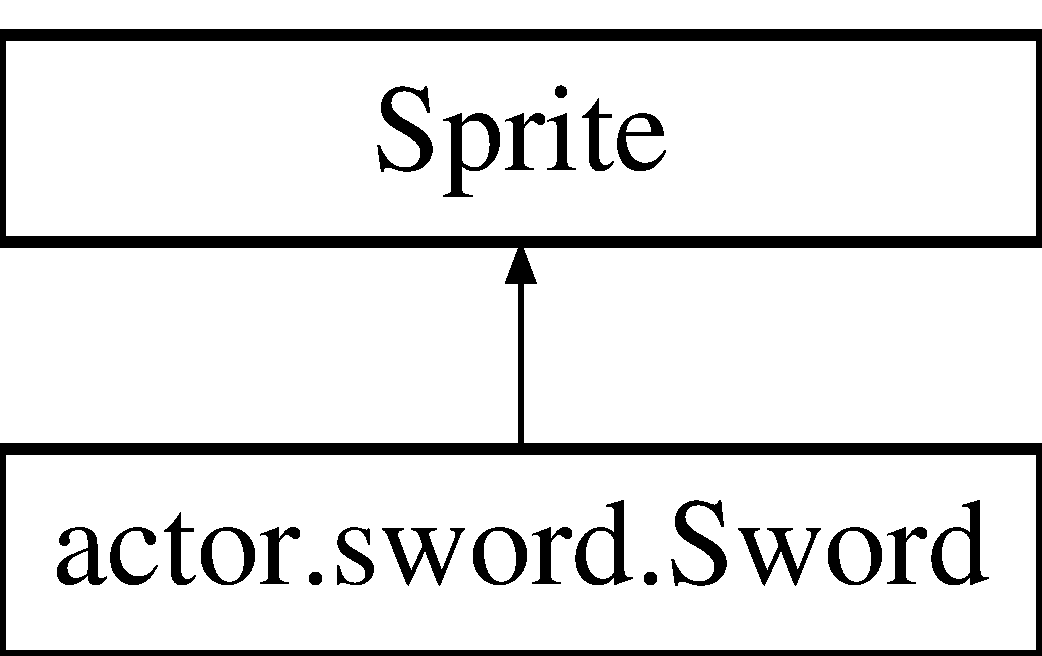
\includegraphics[height=2.000000cm]{classactor_1_1sword_1_1_sword}
\end{center}
\end{figure}
\subsection*{Public Member Functions}
\begin{DoxyCompactItemize}
\item 
def \hyperlink{classactor_1_1sword_1_1_sword_a311383f1e990c512b78b02c1b28cd7ea}{\+\_\+\+\_\+init\+\_\+\+\_\+} (self, x, y, direction)
\begin{DoxyCompactList}\small\item\em \hyperlink{classactor_1_1sword_1_1_sword}{Sword} constructor, taking an x and y coordinate, and the direction for the sword to be pointing (player direction) \end{DoxyCompactList}\end{DoxyCompactItemize}
\subsection*{Public Attributes}
\begin{DoxyCompactItemize}
\item 
\mbox{\Hypertarget{classactor_1_1sword_1_1_sword_a4647017ca649b12ca382614b3af59827}\label{classactor_1_1sword_1_1_sword_a4647017ca649b12ca382614b3af59827}} 
\hyperlink{classactor_1_1sword_1_1_sword_a4647017ca649b12ca382614b3af59827}{sprite}
\begin{DoxyCompactList}\small\item\em Array of all possible sword directions (following usual directional standards, 0-\/3, starting at left going clockwise) \end{DoxyCompactList}\item 
\hyperlink{classactor_1_1sword_1_1_sword_a9fd392562552eb7009662bd7e6701148}{image}
\begin{DoxyCompactList}\small\item\em Sprite image of the sword. \end{DoxyCompactList}\item 
\mbox{\Hypertarget{classactor_1_1sword_1_1_sword_ae79e5ac458440b092db89e72c26c2aa6}\label{classactor_1_1sword_1_1_sword_ae79e5ac458440b092db89e72c26c2aa6}} 
\hyperlink{classactor_1_1sword_1_1_sword_ae79e5ac458440b092db89e72c26c2aa6}{rect}
\begin{DoxyCompactList}\small\item\em X and Y position of the sword. \end{DoxyCompactList}\end{DoxyCompactItemize}


\subsection{Detailed Description}
Player \hyperlink{classactor_1_1sword_1_1_sword}{Sword} Class  Class for the creation and deletion of the sword sprite object, made when the player attacks. 

\subsection{Constructor \& Destructor Documentation}
\mbox{\Hypertarget{classactor_1_1sword_1_1_sword_a311383f1e990c512b78b02c1b28cd7ea}\label{classactor_1_1sword_1_1_sword_a311383f1e990c512b78b02c1b28cd7ea}} 
\index{actor\+::sword\+::\+Sword@{actor\+::sword\+::\+Sword}!\+\_\+\+\_\+init\+\_\+\+\_\+@{\+\_\+\+\_\+init\+\_\+\+\_\+}}
\index{\+\_\+\+\_\+init\+\_\+\+\_\+@{\+\_\+\+\_\+init\+\_\+\+\_\+}!actor\+::sword\+::\+Sword@{actor\+::sword\+::\+Sword}}
\subsubsection{\texorpdfstring{\+\_\+\+\_\+init\+\_\+\+\_\+()}{\_\_init\_\_()}}
{\footnotesize\ttfamily def actor.\+sword.\+Sword.\+\_\+\+\_\+init\+\_\+\+\_\+ (\begin{DoxyParamCaption}\item[{}]{self,  }\item[{}]{x,  }\item[{}]{y,  }\item[{}]{direction }\end{DoxyParamCaption})}



\hyperlink{classactor_1_1sword_1_1_sword}{Sword} constructor, taking an x and y coordinate, and the direction for the sword to be pointing (player direction) 


\begin{DoxyParams}{Parameters}
{\em x} & \hyperlink{classactor_1_1sword_1_1_sword}{Sword}\textquotesingle{}s x coordinate \\
\hline
{\em y} & \hyperlink{classactor_1_1sword_1_1_sword}{Sword}\textquotesingle{}s y coordinate \\
\hline
{\em direction} & \hyperlink{classactor_1_1sword_1_1_sword}{Sword}\textquotesingle{}s direction (integer from 0 to 3, starting left, going clockwise) \\
\hline
\end{DoxyParams}


\subsection{Member Data Documentation}
\mbox{\Hypertarget{classactor_1_1sword_1_1_sword_a9fd392562552eb7009662bd7e6701148}\label{classactor_1_1sword_1_1_sword_a9fd392562552eb7009662bd7e6701148}} 
\index{actor\+::sword\+::\+Sword@{actor\+::sword\+::\+Sword}!image@{image}}
\index{image@{image}!actor\+::sword\+::\+Sword@{actor\+::sword\+::\+Sword}}
\subsubsection{\texorpdfstring{image}{image}}
{\footnotesize\ttfamily actor.\+sword.\+Sword.\+image}



Sprite image of the sword. 

Below is for testing self.\+image = pygame.\+Surface(\mbox{[}26, 14\mbox{]}) self.\+image.\+fill((200, 0, 0)) 

The documentation for this class was generated from the following file\+:\begin{DoxyCompactItemize}
\item 
src/actor/\hyperlink{sword_8py}{sword.\+py}\end{DoxyCompactItemize}

\hypertarget{classcollision_1_1wall_1_1_wall}{}\section{collision.\+wall.\+Wall Class Reference}
\label{classcollision_1_1wall_1_1_wall}\index{collision.\+wall.\+Wall@{collision.\+wall.\+Wall}}


This class represents the \hyperlink{classcollision_1_1wall_1_1_wall}{Wall} class for collision for objects in the environment.  


Inheritance diagram for collision.\+wall.\+Wall\+:\begin{figure}[H]
\begin{center}
\leavevmode
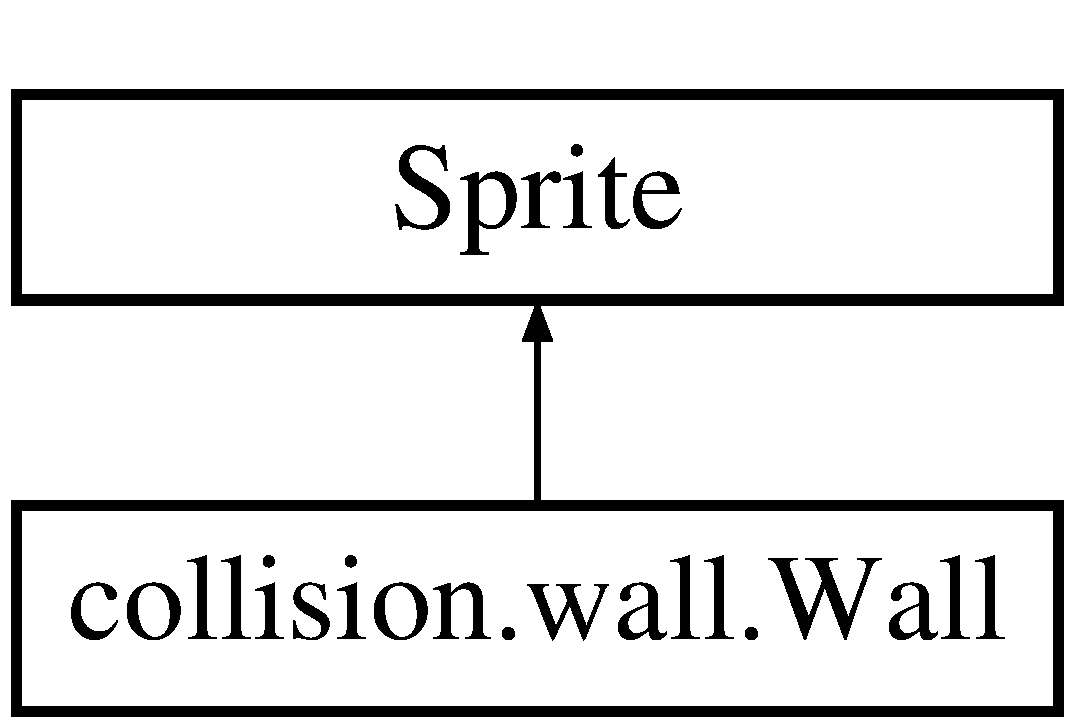
\includegraphics[height=2.000000cm]{classcollision_1_1wall_1_1_wall}
\end{center}
\end{figure}
\subsection*{Public Member Functions}
\begin{DoxyCompactItemize}
\item 
def \hyperlink{classcollision_1_1wall_1_1_wall_a9e55a33a1a456adb22a7dadc4f26be4c}{\+\_\+\+\_\+init\+\_\+\+\_\+} (self, x, y, w, h, sprite)
\begin{DoxyCompactList}\small\item\em Constructor for the \hyperlink{classcollision_1_1wall_1_1_wall}{Wall} class. \end{DoxyCompactList}\item 
def \hyperlink{classcollision_1_1wall_1_1_wall_a9514acfca4d222ec8d838d7bb29aeb1e}{collision} (self, i)
\begin{DoxyCompactList}\small\item\em This method checks for collision with the \hyperlink{classcollision_1_1wall_1_1_wall}{Wall} object and other sprite object. \end{DoxyCompactList}\end{DoxyCompactItemize}
\subsection*{Public Attributes}
\begin{DoxyCompactItemize}
\item 
\hyperlink{classcollision_1_1wall_1_1_wall_ac5d61504c644c284d3fb0b67e9bcc1c3}{image}
\begin{DoxyCompactList}\small\item\em This represents the sprite image for \hyperlink{classcollision_1_1wall_1_1_wall}{Wall} object. \end{DoxyCompactList}\item 
\hyperlink{classcollision_1_1wall_1_1_wall_a7bdfce57724f53f3b0879e12f2f3b78e}{rect}
\begin{DoxyCompactList}\small\item\em This represents rectangle for position for the sprite image of the \hyperlink{classcollision_1_1wall_1_1_wall}{Wall} object. \end{DoxyCompactList}\item 
\hyperlink{classcollision_1_1wall_1_1_wall_aacfb0da0a2fa307f54a571348a0df427}{id}
\begin{DoxyCompactList}\small\item\em This represents the ID for the \hyperlink{classcollision_1_1wall_1_1_wall}{Wall} object, ised for collision in {\bfseries main.\+py}. \end{DoxyCompactList}\end{DoxyCompactItemize}


\subsection{Detailed Description}
This class represents the \hyperlink{classcollision_1_1wall_1_1_wall}{Wall} class for collision for objects in the environment. 

The \hyperlink{classcollision_1_1wall_1_1_wall}{Wall} class uses the base class for visible game objects from Pygame library. 

\subsection{Constructor \& Destructor Documentation}
\mbox{\Hypertarget{classcollision_1_1wall_1_1_wall_a9e55a33a1a456adb22a7dadc4f26be4c}\label{classcollision_1_1wall_1_1_wall_a9e55a33a1a456adb22a7dadc4f26be4c}} 
\index{collision\+::wall\+::\+Wall@{collision\+::wall\+::\+Wall}!\+\_\+\+\_\+init\+\_\+\+\_\+@{\+\_\+\+\_\+init\+\_\+\+\_\+}}
\index{\+\_\+\+\_\+init\+\_\+\+\_\+@{\+\_\+\+\_\+init\+\_\+\+\_\+}!collision\+::wall\+::\+Wall@{collision\+::wall\+::\+Wall}}
\subsubsection{\texorpdfstring{\+\_\+\+\_\+init\+\_\+\+\_\+()}{\_\_init\_\_()}}
{\footnotesize\ttfamily def collision.\+wall.\+Wall.\+\_\+\+\_\+init\+\_\+\+\_\+ (\begin{DoxyParamCaption}\item[{}]{self,  }\item[{}]{x,  }\item[{}]{y,  }\item[{}]{w,  }\item[{}]{h,  }\item[{}]{sprite }\end{DoxyParamCaption})}



Constructor for the \hyperlink{classcollision_1_1wall_1_1_wall}{Wall} class. 

Constructor for \hyperlink{classcollision_1_1wall_1_1_wall}{Wall} class initializes a \hyperlink{classcollision_1_1wall_1_1_wall}{Wall} object based on the x/y location and the width/height of the wall, and the sprite the collision for the wall will be created upon. 
\begin{DoxyParams}{Parameters}
{\em x} & This represents the integer value for the x-\/location for the \hyperlink{classcollision_1_1wall_1_1_wall}{Wall} object to be created. \\
\hline
{\em y} & This represents the integer value for the y-\/location for the \hyperlink{classcollision_1_1wall_1_1_wall}{Wall} object to be created. \\
\hline
{\em w} & This represents the integer value for the width of the \hyperlink{classcollision_1_1wall_1_1_wall}{Wall} object when created. \\
\hline
{\em h} & This represents the integer value for the height of the \hyperlink{classcollision_1_1wall_1_1_wall}{Wall} object when created. \\
\hline
{\em sprite} & This represents the sprite that the collison for a \hyperlink{classcollision_1_1wall_1_1_wall}{Wall} will be present upon at all times. \\
\hline
\end{DoxyParams}


\subsection{Member Function Documentation}
\mbox{\Hypertarget{classcollision_1_1wall_1_1_wall_a9514acfca4d222ec8d838d7bb29aeb1e}\label{classcollision_1_1wall_1_1_wall_a9514acfca4d222ec8d838d7bb29aeb1e}} 
\index{collision\+::wall\+::\+Wall@{collision\+::wall\+::\+Wall}!collision@{collision}}
\index{collision@{collision}!collision\+::wall\+::\+Wall@{collision\+::wall\+::\+Wall}}
\subsubsection{\texorpdfstring{collision()}{collision()}}
{\footnotesize\ttfamily def collision.\+wall.\+Wall.\+collision (\begin{DoxyParamCaption}\item[{}]{self,  }\item[{}]{i }\end{DoxyParamCaption})}



This method checks for collision with the \hyperlink{classcollision_1_1wall_1_1_wall}{Wall} object and other sprite object. 

The collision will be checked with the \hyperlink{classcollision_1_1wall_1_1_wall}{Wall} and other sprite object as the object collides with the wall. 
\begin{DoxyParams}{Parameters}
{\em i} & This is the sprite object that is passed into the method, and checks if the object is colliding with the \hyperlink{classcollision_1_1wall_1_1_wall}{Wall} object, reseting the sprite objects location accordingly. \\
\hline
\end{DoxyParams}


\subsection{Member Data Documentation}
\mbox{\Hypertarget{classcollision_1_1wall_1_1_wall_aacfb0da0a2fa307f54a571348a0df427}\label{classcollision_1_1wall_1_1_wall_aacfb0da0a2fa307f54a571348a0df427}} 
\index{collision\+::wall\+::\+Wall@{collision\+::wall\+::\+Wall}!id@{id}}
\index{id@{id}!collision\+::wall\+::\+Wall@{collision\+::wall\+::\+Wall}}
\subsubsection{\texorpdfstring{id}{id}}
{\footnotesize\ttfamily collision.\+wall.\+Wall.\+id}



This represents the ID for the \hyperlink{classcollision_1_1wall_1_1_wall}{Wall} object, ised for collision in {\bfseries main.\+py}. 

\mbox{\Hypertarget{classcollision_1_1wall_1_1_wall_ac5d61504c644c284d3fb0b67e9bcc1c3}\label{classcollision_1_1wall_1_1_wall_ac5d61504c644c284d3fb0b67e9bcc1c3}} 
\index{collision\+::wall\+::\+Wall@{collision\+::wall\+::\+Wall}!image@{image}}
\index{image@{image}!collision\+::wall\+::\+Wall@{collision\+::wall\+::\+Wall}}
\subsubsection{\texorpdfstring{image}{image}}
{\footnotesize\ttfamily collision.\+wall.\+Wall.\+image}



This represents the sprite image for \hyperlink{classcollision_1_1wall_1_1_wall}{Wall} object. 

\mbox{\Hypertarget{classcollision_1_1wall_1_1_wall_a7bdfce57724f53f3b0879e12f2f3b78e}\label{classcollision_1_1wall_1_1_wall_a7bdfce57724f53f3b0879e12f2f3b78e}} 
\index{collision\+::wall\+::\+Wall@{collision\+::wall\+::\+Wall}!rect@{rect}}
\index{rect@{rect}!collision\+::wall\+::\+Wall@{collision\+::wall\+::\+Wall}}
\subsubsection{\texorpdfstring{rect}{rect}}
{\footnotesize\ttfamily collision.\+wall.\+Wall.\+rect}



This represents rectangle for position for the sprite image of the \hyperlink{classcollision_1_1wall_1_1_wall}{Wall} object. 



The documentation for this class was generated from the following file\+:\begin{DoxyCompactItemize}
\item 
src/collision/\hyperlink{wall_8py}{wall.\+py}\end{DoxyCompactItemize}

\chapter{File Documentation}
\hypertarget{aquamentus_8py}{}\section{src/actor/aquamentus.py File Reference}
\label{aquamentus_8py}\index{src/actor/aquamentus.\+py@{src/actor/aquamentus.\+py}}


Aquamentus Boss  


\subsection*{Classes}
\begin{DoxyCompactItemize}
\item 
class \hyperlink{classactor_1_1aquamentus_1_1_aquamentus}{actor.\+aquamentus.\+Aquamentus}
\begin{DoxyCompactList}\small\item\em This class represents the \hyperlink{classactor_1_1aquamentus_1_1_aquamentus}{Aquamentus} Boss. \end{DoxyCompactList}\end{DoxyCompactItemize}
\subsection*{Functions}
\begin{DoxyCompactItemize}
\item 
def \hyperlink{aquamentus_8py_a2a10f7e1433417e1e65fbcee77760974}{actor.\+aquamentus.\+populate\+Sprites} ()
\begin{DoxyCompactList}\small\item\em Creates the sprite list for \hyperlink{classactor_1_1aquamentus_1_1_aquamentus}{Aquamentus}. \end{DoxyCompactList}\end{DoxyCompactItemize}
\subsection*{Variables}
\begin{DoxyCompactItemize}
\item 
\mbox{\Hypertarget{aquamentus_8py_a478ff4f7934f64bf8969b57158cc897a}\label{aquamentus_8py_a478ff4f7934f64bf8969b57158cc897a}} 
string {\bfseries actor.\+aquamentus.\+S\+P\+R\+I\+T\+E\+\_\+\+M\+AP} = \textquotesingle{}src/actor/sprites/aquamentus.\+png\textquotesingle{}
\end{DoxyCompactItemize}


\subsection{Detailed Description}
Aquamentus Boss 

\begin{DoxyAuthor}{Author}
Giacomo Loparco, Bilal Jaffry, Lucas Zacharewicz 
\end{DoxyAuthor}
\begin{DoxyDate}{Date}
November 8 2018 
\end{DoxyDate}


\subsection{Function Documentation}
\mbox{\Hypertarget{aquamentus_8py_file_a2a10f7e1433417e1e65fbcee77760974}\label{aquamentus_8py_file_a2a10f7e1433417e1e65fbcee77760974}} 
\index{aquamentus.\+py@{aquamentus.\+py}!populate\+Sprites@{populate\+Sprites}}
\index{populate\+Sprites@{populate\+Sprites}!aquamentus.\+py@{aquamentus.\+py}}
\subsubsection{\texorpdfstring{populate\+Sprites()}{populateSprites()}}
{\footnotesize\ttfamily def actor.\+aquamentus.\+populate\+Sprites (\begin{DoxyParamCaption}{ }\end{DoxyParamCaption})}



Creates the sprite list for Aquamentus. 

Iterates through a sprite sheet to pull images for the sprite array \begin{DoxyReturn}{Returns}
sprites Array if the sprites that represent the Aquamentus 
\end{DoxyReturn}

\hypertarget{boomerang_8py}{}\section{src/actor/boomerang.py File Reference}
\label{boomerang_8py}\index{src/actor/boomerang.\+py@{src/actor/boomerang.\+py}}


Boomerang Weapon  


\subsection*{Classes}
\begin{DoxyCompactItemize}
\item 
class \hyperlink{classactor_1_1boomerang_1_1_boomerang}{actor.\+boomerang.\+Boomerang}
\begin{DoxyCompactList}\small\item\em \hyperlink{classactor_1_1boomerang_1_1_boomerang}{Boomerang} Weapon Class  The class holding the creation, behaviour, and collision effects of the player\textquotesingle{}s boomerang weapon. \end{DoxyCompactList}\end{DoxyCompactItemize}
\subsection*{Functions}
\begin{DoxyCompactItemize}
\item 
def \hyperlink{boomerang_8py_a8d197eab0bf6f54621960f429f24f0b5}{actor.\+boomerang.\+populate\+Sprites} ()
\begin{DoxyCompactList}\small\item\em Creates the sprite list for \hyperlink{classactor_1_1boomerang_1_1_boomerang}{Boomerang}. \end{DoxyCompactList}\item 
def \hyperlink{boomerang_8py_a34a1a69f80c09f481480afccdc2f460a}{actor.\+boomerang.\+stuncoeffient} (x)
\begin{DoxyCompactList}\small\item\em Finds the coeffient for the stun value  Uses a quadradic equation with the frame counter to find the coefficent. \end{DoxyCompactList}\end{DoxyCompactItemize}
\subsection*{Variables}
\begin{DoxyCompactItemize}
\item 
\mbox{\Hypertarget{boomerang_8py_a6f92a4644bc9f8e6b3bb23b154ddabfc}\label{boomerang_8py_a6f92a4644bc9f8e6b3bb23b154ddabfc}} 
string {\bfseries actor.\+boomerang.\+S\+P\+R\+I\+T\+E\+\_\+\+M\+AP} = \textquotesingle{}src/actor/sprites/boomerang.\+png\textquotesingle{}
\end{DoxyCompactItemize}


\subsection{Detailed Description}
Boomerang Weapon 

\begin{DoxyAuthor}{Author}
Giacomo Loparco, Bilal Jaffry, Lucas Zacharewicz 
\end{DoxyAuthor}
\begin{DoxyDate}{Date}
November 6 2018 
\end{DoxyDate}


\subsection{Function Documentation}
\mbox{\Hypertarget{boomerang_8py_file_a8d197eab0bf6f54621960f429f24f0b5}\label{boomerang_8py_file_a8d197eab0bf6f54621960f429f24f0b5}} 
\index{boomerang.\+py@{boomerang.\+py}!populate\+Sprites@{populate\+Sprites}}
\index{populate\+Sprites@{populate\+Sprites}!boomerang.\+py@{boomerang.\+py}}
\subsubsection{\texorpdfstring{populate\+Sprites()}{populateSprites()}}
{\footnotesize\ttfamily def actor.\+boomerang.\+populate\+Sprites (\begin{DoxyParamCaption}{ }\end{DoxyParamCaption})}



Creates the sprite list for Boomerang. 

Iterates through a sprite sheet to pull images for the sprite array \begin{DoxyReturn}{Returns}
sprites Array if the sprites that represent the Boomerang 
\end{DoxyReturn}
\mbox{\Hypertarget{boomerang_8py_file_a34a1a69f80c09f481480afccdc2f460a}\label{boomerang_8py_file_a34a1a69f80c09f481480afccdc2f460a}} 
\index{boomerang.\+py@{boomerang.\+py}!stuncoeffient@{stuncoeffient}}
\index{stuncoeffient@{stuncoeffient}!boomerang.\+py@{boomerang.\+py}}
\subsubsection{\texorpdfstring{stuncoeffient()}{stuncoeffient()}}
{\footnotesize\ttfamily def actor.\+boomerang.\+stuncoeffient (\begin{DoxyParamCaption}\item[{}]{x }\end{DoxyParamCaption})}



Finds the coeffient for the stun value  Uses a quadradic equation with the frame counter to find the coefficent. 


\begin{DoxyParams}{Parameters}
{\em x} & The current frame of the boomerang \\
\hline
\end{DoxyParams}
\begin{DoxyReturn}{Returns}
c The coefficent for the boomerang stun 
\end{DoxyReturn}

\hypertarget{boss_8py}{}\section{src/actor/boss.py File Reference}
\label{boss_8py}\index{src/actor/boss.\+py@{src/actor/boss.\+py}}


Boss Template  


\subsection*{Classes}
\begin{DoxyCompactItemize}
\item 
class \hyperlink{classactor_1_1boss_1_1_boss}{actor.\+boss.\+Boss}
\begin{DoxyCompactList}\small\item\em Superclass for representing a \hyperlink{classactor_1_1boss_1_1_boss}{Boss}. \end{DoxyCompactList}\end{DoxyCompactItemize}


\subsection{Detailed Description}
Boss Template 

\begin{DoxyAuthor}{Author}
Giacomo Loparco, Bilal Jaffry, Lucas Zacharewicz 
\end{DoxyAuthor}
\begin{DoxyDate}{Date}
November 7 2018 
\end{DoxyDate}

\hypertarget{constants_8py}{}\section{src/actor/constants.py File Reference}
\label{constants_8py}\index{src/actor/constants.\+py@{src/actor/constants.\+py}}


Actor Constants  


\subsection*{Variables}
\begin{DoxyCompactItemize}
\item 
\mbox{\Hypertarget{constants_8py_ae71d2029c380cc32edb39761eea144c7}\label{constants_8py_ae71d2029c380cc32edb39761eea144c7}} 
tuple \hyperlink{constants_8py_ae71d2029c380cc32edb39761eea144c7}{actor.\+constants.\+B\+L\+A\+CK} = (0,0,0)
\begin{DoxyCompactList}\small\item\em Defines the colour black. \end{DoxyCompactList}\item 
\mbox{\Hypertarget{constants_8py_ae679126f031fb5e4b7b7052cebc007f5}\label{constants_8py_ae679126f031fb5e4b7b7052cebc007f5}} 
tuple \hyperlink{constants_8py_ae679126f031fb5e4b7b7052cebc007f5}{actor.\+constants.\+W\+H\+I\+TE} = (255, 255, 255)
\begin{DoxyCompactList}\small\item\em Defines the colour white. \end{DoxyCompactList}\item 
\mbox{\Hypertarget{constants_8py_a0695b37bc9ae4be561603acef62e0c68}\label{constants_8py_a0695b37bc9ae4be561603acef62e0c68}} 
tuple \hyperlink{constants_8py_a0695b37bc9ae4be561603acef62e0c68}{actor.\+constants.\+P\+U\+R\+P\+LE} = (255, 50, 255)
\begin{DoxyCompactList}\small\item\em Defines the colour purple. \end{DoxyCompactList}\item 
\mbox{\Hypertarget{constants_8py_aba1696eb35fbc68af86408867b31bae7}\label{constants_8py_aba1696eb35fbc68af86408867b31bae7}} 
tuple \hyperlink{constants_8py_aba1696eb35fbc68af86408867b31bae7}{actor.\+constants.\+R\+ED} = (255, 50, 50)
\begin{DoxyCompactList}\small\item\em Defines the colour red. \end{DoxyCompactList}\item 
\mbox{\Hypertarget{constants_8py_a5d7243c9c2aed56f435132ef62b0c7ac}\label{constants_8py_a5d7243c9c2aed56f435132ef62b0c7ac}} 
tuple \hyperlink{constants_8py_a5d7243c9c2aed56f435132ef62b0c7ac}{actor.\+constants.\+B\+L\+UE} = (0,0,255)
\begin{DoxyCompactList}\small\item\em Defines the color blue. \end{DoxyCompactList}\item 
\mbox{\Hypertarget{constants_8py_a64ae3dfc2b38d5bb0ec434214290f630}\label{constants_8py_a64ae3dfc2b38d5bb0ec434214290f630}} 
int \hyperlink{constants_8py_a64ae3dfc2b38d5bb0ec434214290f630}{actor.\+constants.\+P\+L\+A\+Y\+E\+R\+\_\+\+W\+I\+D\+TH} = 15
\begin{DoxyCompactList}\small\item\em Defines the player\textquotesingle{}s width. \end{DoxyCompactList}\item 
\mbox{\Hypertarget{constants_8py_a55e4ca1a569ea8638da052b2df17f71d}\label{constants_8py_a55e4ca1a569ea8638da052b2df17f71d}} 
int \hyperlink{constants_8py_a55e4ca1a569ea8638da052b2df17f71d}{actor.\+constants.\+P\+L\+A\+Y\+E\+R\+\_\+\+H\+E\+I\+G\+HT} = 15
\begin{DoxyCompactList}\small\item\em Defines the player\textquotesingle{}s height. \end{DoxyCompactList}\item 
\mbox{\Hypertarget{constants_8py_acfa1b36f657fbaa9eadc9af635c11855}\label{constants_8py_acfa1b36f657fbaa9eadc9af635c11855}} 
int \hyperlink{constants_8py_acfa1b36f657fbaa9eadc9af635c11855}{actor.\+constants.\+P\+L\+A\+Y\+E\+R\+\_\+\+S\+P\+E\+ED} = 2
\begin{DoxyCompactList}\small\item\em Defines the player\textquotesingle{}s speed. \end{DoxyCompactList}\item 
\mbox{\Hypertarget{constants_8py_a70070536899bc058cb90821397728a10}\label{constants_8py_a70070536899bc058cb90821397728a10}} 
int \hyperlink{constants_8py_a70070536899bc058cb90821397728a10}{actor.\+constants.\+P\+L\+A\+Y\+E\+R\+\_\+\+M\+A\+X\+\_\+\+HP} = 3
\begin{DoxyCompactList}\small\item\em Defines the player\textquotesingle{}s max hp. \end{DoxyCompactList}\item 
\mbox{\Hypertarget{constants_8py_a8d40555767665b05f87d70c5c0572005}\label{constants_8py_a8d40555767665b05f87d70c5c0572005}} 
int \hyperlink{constants_8py_a8d40555767665b05f87d70c5c0572005}{actor.\+constants.\+P\+L\+A\+Y\+E\+R\+\_\+\+D\+O\+O\+R\+C\+O\+U\+NT} = 20
\begin{DoxyCompactList}\small\item\em Defines how many frames the player collides with a locked door before a key is used. \end{DoxyCompactList}\item 
\mbox{\Hypertarget{constants_8py_aee5a4b60ba93c9c3295946acb6e9496f}\label{constants_8py_aee5a4b60ba93c9c3295946acb6e9496f}} 
int \hyperlink{constants_8py_aee5a4b60ba93c9c3295946acb6e9496f}{actor.\+constants.\+P\+L\+A\+Y\+E\+R\+\_\+\+S\+P\+A\+W\+N\+C\+O\+U\+NT} = 8
\begin{DoxyCompactList}\small\item\em Defines how long the player is uncontrollable for when entering a new room (movement to walk out of door) \end{DoxyCompactList}\item 
\mbox{\Hypertarget{constants_8py_a9c1056060510048b07f32fb99ca8b93e}\label{constants_8py_a9c1056060510048b07f32fb99ca8b93e}} 
int \hyperlink{constants_8py_a9c1056060510048b07f32fb99ca8b93e}{actor.\+constants.\+H\+I\+T\+\_\+\+S\+P\+E\+ED} = 12
\begin{DoxyCompactList}\small\item\em Defines the speed of the knock back applied per frame. \end{DoxyCompactList}\item 
\mbox{\Hypertarget{constants_8py_a1ce3bee717c1f2397fa5bf2231469675}\label{constants_8py_a1ce3bee717c1f2397fa5bf2231469675}} 
int \hyperlink{constants_8py_a1ce3bee717c1f2397fa5bf2231469675}{actor.\+constants.\+H\+I\+T\+\_\+\+T\+I\+ME} = 5
\begin{DoxyCompactList}\small\item\em Defines the number of frames hit speed is applied for. \end{DoxyCompactList}\item 
\mbox{\Hypertarget{constants_8py_a0d0f589e01cad8a0a5ef1a54253bcf13}\label{constants_8py_a0d0f589e01cad8a0a5ef1a54253bcf13}} 
int \hyperlink{constants_8py_a0d0f589e01cad8a0a5ef1a54253bcf13}{actor.\+constants.\+H\+I\+T\+\_\+\+I\+F\+R\+A\+ME} = 30
\begin{DoxyCompactList}\small\item\em Defines the number of iframes. \end{DoxyCompactList}\item 
\mbox{\Hypertarget{constants_8py_ab4602bdb853159facf6971c2f7daec55}\label{constants_8py_ab4602bdb853159facf6971c2f7daec55}} 
int \hyperlink{constants_8py_ab4602bdb853159facf6971c2f7daec55}{actor.\+constants.\+A\+T\+K\+\_\+\+W\+I\+D\+TH} = 15
\begin{DoxyCompactList}\small\item\em Defines the width of the attack hitbox. \end{DoxyCompactList}\item 
\mbox{\Hypertarget{constants_8py_af8a4f20f7d0cc886ded420fdccd62469}\label{constants_8py_af8a4f20f7d0cc886ded420fdccd62469}} 
int \hyperlink{constants_8py_af8a4f20f7d0cc886ded420fdccd62469}{actor.\+constants.\+A\+T\+K\+\_\+\+H\+E\+I\+G\+HT} = 15
\begin{DoxyCompactList}\small\item\em Defines the height of the attack hitbox. \end{DoxyCompactList}\item 
\mbox{\Hypertarget{constants_8py_ae1aa209a8b0a492caf4f0567b0dad1b6}\label{constants_8py_ae1aa209a8b0a492caf4f0567b0dad1b6}} 
int \hyperlink{constants_8py_ae1aa209a8b0a492caf4f0567b0dad1b6}{actor.\+constants.\+A\+T\+K\+\_\+\+L\+E\+N\+G\+TH} = 10
\begin{DoxyCompactList}\small\item\em Defines the number of frames the hit stays out for. \end{DoxyCompactList}\item 
\mbox{\Hypertarget{constants_8py_a93a5a6694fa613e1a2385a3c936809db}\label{constants_8py_a93a5a6694fa613e1a2385a3c936809db}} 
int \hyperlink{constants_8py_a93a5a6694fa613e1a2385a3c936809db}{actor.\+constants.\+A\+T\+K\+\_\+\+B\+U\+F\+F\+ER} = 20
\begin{DoxyCompactList}\small\item\em Defines the number of frames before the next attack can start. \end{DoxyCompactList}\item 
\mbox{\Hypertarget{constants_8py_a0aead92b9865fc807173af637b365530}\label{constants_8py_a0aead92b9865fc807173af637b365530}} 
int \hyperlink{constants_8py_a0aead92b9865fc807173af637b365530}{actor.\+constants.\+B\+O\+O\+M\+\_\+\+S\+P\+E\+ED} = 9
\begin{DoxyCompactList}\small\item\em Defines the bommerang speed. \end{DoxyCompactList}\item 
\mbox{\Hypertarget{constants_8py_a18ae93c0c81c57a2de047bf6d0eef0a3}\label{constants_8py_a18ae93c0c81c57a2de047bf6d0eef0a3}} 
float \hyperlink{constants_8py_a18ae93c0c81c57a2de047bf6d0eef0a3}{actor.\+constants.\+B\+O\+O\+M\+\_\+\+R\+E\+T\+U\+RN} = 0.\+3
\begin{DoxyCompactList}\small\item\em Defines the acceleration in the opposite direction of the bommerang\textquotesingle{}s travel path. \end{DoxyCompactList}\item 
\mbox{\Hypertarget{constants_8py_ab3529cfd84b6fa799b34da57d6487c89}\label{constants_8py_ab3529cfd84b6fa799b34da57d6487c89}} 
int \hyperlink{constants_8py_ab3529cfd84b6fa799b34da57d6487c89}{actor.\+constants.\+G\+L\+O\+B\+A\+L\+\_\+\+F\+R\+A\+M\+E\+\_\+\+B\+U\+F\+F\+ER} = 12
\begin{DoxyCompactList}\small\item\em Coordinate Divisor that determines range in which next sprite should render. \end{DoxyCompactList}\item 
\mbox{\Hypertarget{constants_8py_ae87d798b9e0dfce36114c5efd5a79efd}\label{constants_8py_ae87d798b9e0dfce36114c5efd5a79efd}} 
int \hyperlink{constants_8py_ae87d798b9e0dfce36114c5efd5a79efd}{actor.\+constants.\+K\+E\+E\+S\+E\+\_\+\+M\+A\+X\+\_\+\+HP} = 1
\begin{DoxyCompactList}\small\item\em Defines the keese\textquotesingle{}s max hp. \end{DoxyCompactList}\item 
\mbox{\Hypertarget{constants_8py_aac73f9ade593b01a50d64b5c5cab762f}\label{constants_8py_aac73f9ade593b01a50d64b5c5cab762f}} 
float \hyperlink{constants_8py_aac73f9ade593b01a50d64b5c5cab762f}{actor.\+constants.\+K\+E\+E\+S\+E\+\_\+\+D\+MG} = 0.\+5
\begin{DoxyCompactList}\small\item\em Defines the keese\textquotesingle{}s damage. \end{DoxyCompactList}\item 
\mbox{\Hypertarget{constants_8py_a769b7abc804a214b43c5f235db8f9f43}\label{constants_8py_a769b7abc804a214b43c5f235db8f9f43}} 
int \hyperlink{constants_8py_a769b7abc804a214b43c5f235db8f9f43}{actor.\+constants.\+K\+E\+E\+S\+E\+\_\+\+M\+A\+X\+\_\+\+S\+P\+E\+ED} = 2
\begin{DoxyCompactList}\small\item\em Defines the keese\textquotesingle{}s max speed. \end{DoxyCompactList}\item 
\mbox{\Hypertarget{constants_8py_ab652b667f5566e379eed42daf759b3f0}\label{constants_8py_ab652b667f5566e379eed42daf759b3f0}} 
int \hyperlink{constants_8py_ab652b667f5566e379eed42daf759b3f0}{actor.\+constants.\+K\+E\+E\+S\+E\+\_\+\+M\+I\+N\+\_\+\+S\+P\+E\+ED} = 1
\begin{DoxyCompactList}\small\item\em Defines the keese\textquotesingle{}s min speed. \end{DoxyCompactList}\item 
\mbox{\Hypertarget{constants_8py_a8cdbc33ae8c0cd8299fea64e6584cbb2}\label{constants_8py_a8cdbc33ae8c0cd8299fea64e6584cbb2}} 
int \hyperlink{constants_8py_a8cdbc33ae8c0cd8299fea64e6584cbb2}{actor.\+constants.\+A\+C\+C\+E\+P\+T\+A\+B\+L\+E\+\_\+\+R\+A\+D\+I\+US} = 20
\begin{DoxyCompactList}\small\item\em Defines the keese\textquotesingle{}s minimum magnitude from its determined travel point before stopping. \end{DoxyCompactList}\item 
\mbox{\Hypertarget{constants_8py_ab460931b2f8a7565fd455700d80ca1c2}\label{constants_8py_ab460931b2f8a7565fd455700d80ca1c2}} 
int \hyperlink{constants_8py_ab460931b2f8a7565fd455700d80ca1c2}{actor.\+constants.\+K\+E\+E\+S\+E\+\_\+\+M\+A\+G\+N\+I\+T\+U\+D\+E\+\_\+\+M\+IN} = 200
\begin{DoxyCompactList}\small\item\em Defines the keese\textquotesingle{}s minimum magnitude for selecting its next travel point. \end{DoxyCompactList}\item 
\mbox{\Hypertarget{constants_8py_a61050d208cd3f976497edcd0c9460ba0}\label{constants_8py_a61050d208cd3f976497edcd0c9460ba0}} 
int \hyperlink{constants_8py_a61050d208cd3f976497edcd0c9460ba0}{actor.\+constants.\+S\+T\+A\+L\+F\+O\+S\+\_\+\+M\+A\+X\+\_\+\+HP} = 2
\begin{DoxyCompactList}\small\item\em Defines the stalfos\textquotesingle{} max hp. \end{DoxyCompactList}\item 
\mbox{\Hypertarget{constants_8py_ab4f14982f7642c46aa78f94abeb4bc6b}\label{constants_8py_ab4f14982f7642c46aa78f94abeb4bc6b}} 
int \hyperlink{constants_8py_ab4f14982f7642c46aa78f94abeb4bc6b}{actor.\+constants.\+S\+T\+A\+L\+F\+O\+S\+\_\+\+D\+MG} = 1
\begin{DoxyCompactList}\small\item\em Defines the stalfos\textquotesingle{} damage. \end{DoxyCompactList}\item 
\mbox{\Hypertarget{constants_8py_adf85e68c9f7682e6e3f58876a0eac461}\label{constants_8py_adf85e68c9f7682e6e3f58876a0eac461}} 
int \hyperlink{constants_8py_adf85e68c9f7682e6e3f58876a0eac461}{actor.\+constants.\+S\+T\+A\+L\+F\+O\+S\+\_\+\+S\+P\+E\+ED} = 1
\begin{DoxyCompactList}\small\item\em Defines the stalfos\textquotesingle{} speed. \end{DoxyCompactList}\item 
\mbox{\Hypertarget{constants_8py_a2b2fa6dcc70e36ce456b3ec1acdd5c0a}\label{constants_8py_a2b2fa6dcc70e36ce456b3ec1acdd5c0a}} 
int \hyperlink{constants_8py_a2b2fa6dcc70e36ce456b3ec1acdd5c0a}{actor.\+constants.\+S\+T\+A\+L\+F\+O\+S\+\_\+\+H\+I\+T\+\_\+\+S\+P\+E\+ED} = 10
\begin{DoxyCompactList}\small\item\em Defines the stalfos\textquotesingle{} speed during knockback. \end{DoxyCompactList}\item 
\mbox{\Hypertarget{constants_8py_a74ebaa78c2254154db22bc2b26ac5ec4}\label{constants_8py_a74ebaa78c2254154db22bc2b26ac5ec4}} 
int \hyperlink{constants_8py_a74ebaa78c2254154db22bc2b26ac5ec4}{actor.\+constants.\+E\+N\+E\+M\+Y\+\_\+\+S\+T\+U\+N\+C\+O\+U\+NT} = 35
\begin{DoxyCompactList}\small\item\em Length of frames an enemy will be stunned for when hit by a boomerang. \end{DoxyCompactList}\item 
\mbox{\Hypertarget{constants_8py_a6798a2ba15f37026a428d4ae33b36385}\label{constants_8py_a6798a2ba15f37026a428d4ae33b36385}} 
int \hyperlink{constants_8py_a6798a2ba15f37026a428d4ae33b36385}{actor.\+constants.\+A\+Q\+U\+A\+M\+E\+N\+T\+U\+S\+\_\+\+M\+A\+X\+\_\+\+HP} = 5
\begin{DoxyCompactList}\small\item\em Defines the aquamentus\textquotesingle{} max hp. \end{DoxyCompactList}\item 
\mbox{\Hypertarget{constants_8py_a1af2813819c1f74c0c03e4c28e688c7e}\label{constants_8py_a1af2813819c1f74c0c03e4c28e688c7e}} 
int \hyperlink{constants_8py_a1af2813819c1f74c0c03e4c28e688c7e}{actor.\+constants.\+A\+Q\+U\+A\+M\+E\+N\+T\+U\+S\+\_\+\+D\+MG} = 2
\begin{DoxyCompactList}\small\item\em Defines the aquamentus\textquotesingle{} damage. \end{DoxyCompactList}\item 
\mbox{\Hypertarget{constants_8py_afd41761bdc5ad8caadf945e8a0dd3e7c}\label{constants_8py_afd41761bdc5ad8caadf945e8a0dd3e7c}} 
int \hyperlink{constants_8py_afd41761bdc5ad8caadf945e8a0dd3e7c}{actor.\+constants.\+A\+Q\+U\+A\+M\+E\+N\+T\+U\+S\+\_\+\+S\+P\+E\+ED} = 1
\begin{DoxyCompactList}\small\item\em Defines the aquamentus\textquotesingle{} speed. \end{DoxyCompactList}\item 
\mbox{\Hypertarget{constants_8py_ab459379ba3104f11ba93721fc14c2c7c}\label{constants_8py_ab459379ba3104f11ba93721fc14c2c7c}} 
int \hyperlink{constants_8py_ab459379ba3104f11ba93721fc14c2c7c}{actor.\+constants.\+F\+I\+R\+E\+B\+A\+L\+L\+\_\+\+D\+MG} = 1
\begin{DoxyCompactList}\small\item\em Defines the fireballs damage. \end{DoxyCompactList}\end{DoxyCompactItemize}


\subsection{Detailed Description}
Actor Constants 

\begin{DoxyAuthor}{Author}
Giacomo Loparco, Bilal Jaffry, Lucas Zacharewicz 
\end{DoxyAuthor}
\begin{DoxyDate}{Date}
November 7 2018
\end{DoxyDate}
\begin{DoxyAuthor}{Author}
Giacomo Loparco, Bilal Jaffry, Lucas Zacharewicz 
\end{DoxyAuthor}
\begin{DoxyDate}{Date}
November 9 2018 
\end{DoxyDate}

\hypertarget{enemy_8py}{}\section{src/actor/enemy.py File Reference}
\label{enemy_8py}\index{src/actor/enemy.\+py@{src/actor/enemy.\+py}}


Enemy Template  


\subsection*{Classes}
\begin{DoxyCompactItemize}
\item 
class \hyperlink{classactor_1_1enemy_1_1_enemy}{actor.\+enemy.\+Enemy}
\begin{DoxyCompactList}\small\item\em Superclass for representing an \hyperlink{classactor_1_1enemy_1_1_enemy}{Enemy}. \end{DoxyCompactList}\end{DoxyCompactItemize}


\subsection{Detailed Description}
Enemy Template 

\begin{DoxyAuthor}{Author}
Giacomo Loparco, Bilal Jaffry, Lucas Zacharewicz 
\end{DoxyAuthor}
\begin{DoxyDate}{Date}
November 7 2018 
\end{DoxyDate}

\hypertarget{fireball_8py}{}\section{src/actor/fireball.py File Reference}
\label{fireball_8py}\index{src/actor/fireball.\+py@{src/actor/fireball.\+py}}


Fireball object  


\subsection*{Classes}
\begin{DoxyCompactItemize}
\item 
class \hyperlink{classactor_1_1fireball_1_1_fireball}{actor.\+fireball.\+Fireball}
\begin{DoxyCompactList}\small\item\em This class represents the \hyperlink{classactor_1_1fireball_1_1_fireball}{Fireball} object. \end{DoxyCompactList}\end{DoxyCompactItemize}
\subsection*{Functions}
\begin{DoxyCompactItemize}
\item 
def \hyperlink{fireball_8py_add7cb65715bca6402d2923671e4c5542}{actor.\+fireball.\+populate\+Sprites} ()
\begin{DoxyCompactList}\small\item\em Creates the sprite list for \hyperlink{classactor_1_1fireball_1_1_fireball}{Fireball}. \end{DoxyCompactList}\end{DoxyCompactItemize}
\subsection*{Variables}
\begin{DoxyCompactItemize}
\item 
\mbox{\Hypertarget{fireball_8py_a230ba1787164cd045f5e07eaf57a1d51}\label{fireball_8py_a230ba1787164cd045f5e07eaf57a1d51}} 
string {\bfseries actor.\+fireball.\+S\+P\+R\+I\+T\+E\+\_\+\+M\+AP} = \textquotesingle{}src/actor/sprites/fireball.\+png\textquotesingle{}
\end{DoxyCompactItemize}


\subsection{Detailed Description}
Fireball object 

\begin{DoxyAuthor}{Author}
Giacomo Loparco, Bilal Jaffry, Lucas Zacharewicz 
\end{DoxyAuthor}
\begin{DoxyDate}{Date}
November 7 2018 
\end{DoxyDate}


\subsection{Function Documentation}
\mbox{\Hypertarget{fireball_8py_file_add7cb65715bca6402d2923671e4c5542}\label{fireball_8py_file_add7cb65715bca6402d2923671e4c5542}} 
\index{fireball.\+py@{fireball.\+py}!populate\+Sprites@{populate\+Sprites}}
\index{populate\+Sprites@{populate\+Sprites}!fireball.\+py@{fireball.\+py}}
\subsubsection{\texorpdfstring{populate\+Sprites()}{populateSprites()}}
{\footnotesize\ttfamily def actor.\+fireball.\+populate\+Sprites (\begin{DoxyParamCaption}{ }\end{DoxyParamCaption})}



Creates the sprite list for Fireball. 

Iterates through a sprite sheet to pull images for the sprite array \begin{DoxyReturn}{Returns}
sprites Array if the sprites that represent the Fireball 
\end{DoxyReturn}

\hypertarget{healthbar_8py}{}\section{src/actor/healthbar.py File Reference}
\label{healthbar_8py}\index{src/actor/healthbar.\+py@{src/actor/healthbar.\+py}}


Health\+Bar Class  


\subsection*{Classes}
\begin{DoxyCompactItemize}
\item 
class \hyperlink{classactor_1_1healthbar_1_1_health___bar}{actor.\+healthbar.\+Health\+\_\+\+Bar}
\begin{DoxyCompactList}\small\item\em This class represents the Health\+Bar for the user controlled player character. \end{DoxyCompactList}\end{DoxyCompactItemize}


\subsection{Detailed Description}
Health\+Bar Class 

\begin{DoxyAuthor}{Author}
Giacomo Loparco, Bilal Jaffry, Lucas Zacharewicz 
\end{DoxyAuthor}
\begin{DoxyDate}{Date}
November 7 2018 
\end{DoxyDate}

\hypertarget{item_8py}{}\section{src/actor/item.py File Reference}
\label{item_8py}\index{src/actor/item.\+py@{src/actor/item.\+py}}


Consumable Items  


\subsection*{Classes}
\begin{DoxyCompactItemize}
\item 
class \hyperlink{classactor_1_1item_1_1_item}{actor.\+item.\+Item}
\begin{DoxyCompactList}\small\item\em Consumable \hyperlink{classactor_1_1item_1_1_item}{Item} Class  This class is used for the creation of a random consumable item, spawned once an enemy has been defeated on their last position before despawn. \end{DoxyCompactList}\end{DoxyCompactItemize}


\subsection{Detailed Description}
Consumable Items 

\begin{DoxyAuthor}{Author}
Giacomo Loparco, Bilal Jaffry, Lucas Zacharewicz 
\end{DoxyAuthor}
\begin{DoxyDate}{Date}
November 6 2018 
\end{DoxyDate}

\hypertarget{keese_8py}{}\section{src/actor/keese.py File Reference}
\label{keese_8py}\index{src/actor/keese.\+py@{src/actor/keese.\+py}}


Keese Enemy  


\subsection*{Classes}
\begin{DoxyCompactItemize}
\item 
class \hyperlink{classactor_1_1keese_1_1_keese}{actor.\+keese.\+Keese}
\begin{DoxyCompactList}\small\item\em This class represents the \hyperlink{classactor_1_1keese_1_1_keese}{Keese} enemy. \end{DoxyCompactList}\end{DoxyCompactItemize}
\subsection*{Functions}
\begin{DoxyCompactItemize}
\item 
def \hyperlink{keese_8py_abcc83e84f82a3614b58fffe875eb6f9e}{actor.\+keese.\+populate\+Sprites} ()
\begin{DoxyCompactList}\small\item\em Creates the sprite list for \hyperlink{classactor_1_1keese_1_1_keese}{Keese}. \end{DoxyCompactList}\end{DoxyCompactItemize}
\subsection*{Variables}
\begin{DoxyCompactItemize}
\item 
\mbox{\Hypertarget{keese_8py_a4dad1f53bfd2a9018931a08b90df8b7e}\label{keese_8py_a4dad1f53bfd2a9018931a08b90df8b7e}} 
string {\bfseries actor.\+keese.\+S\+P\+R\+I\+T\+E\+\_\+\+M\+AP} = \textquotesingle{}src/actor/sprites/keese.\+png\textquotesingle{}
\end{DoxyCompactItemize}


\subsection{Detailed Description}
Keese Enemy 

\begin{DoxyAuthor}{Author}
Giacomo Loparco, Bilal Jaffry, Lucas Zacharewicz 
\end{DoxyAuthor}
\begin{DoxyDate}{Date}
November 7 2018 
\end{DoxyDate}


\subsection{Function Documentation}
\mbox{\Hypertarget{keese_8py_file_abcc83e84f82a3614b58fffe875eb6f9e}\label{keese_8py_file_abcc83e84f82a3614b58fffe875eb6f9e}} 
\index{keese.\+py@{keese.\+py}!populate\+Sprites@{populate\+Sprites}}
\index{populate\+Sprites@{populate\+Sprites}!keese.\+py@{keese.\+py}}
\subsubsection{\texorpdfstring{populate\+Sprites()}{populateSprites()}}
{\footnotesize\ttfamily def actor.\+keese.\+populate\+Sprites (\begin{DoxyParamCaption}{ }\end{DoxyParamCaption})}



Creates the sprite list for Keese. 

Iterates through a sprite sheet to pull images for the sprite array \begin{DoxyReturn}{Returns}
sprites Array if the sprites that represent the Keese 
\end{DoxyReturn}

\hypertarget{player_8py}{}\section{src/actor/player.py File Reference}
\label{player_8py}\index{src/actor/player.\+py@{src/actor/player.\+py}}


Playable Characer  


\subsection*{Classes}
\begin{DoxyCompactItemize}
\item 
class \hyperlink{classactor_1_1player_1_1_player}{actor.\+player.\+Player}
\begin{DoxyCompactList}\small\item\em \hyperlink{classactor_1_1player_1_1_player}{Player} Class  A pygame sprite subclass for defining the creation of the game\textquotesingle{}s playable character, as well as its interactions with both the user and other entities within the game. \end{DoxyCompactList}\end{DoxyCompactItemize}


\subsection{Detailed Description}
Playable Characer 

\begin{DoxyAuthor}{Author}
Giacomo Loparco, Bilal Jaffry, Lucas Zacharewicz 
\end{DoxyAuthor}
\begin{DoxyDate}{Date}
November 6 2018 
\end{DoxyDate}

\hypertarget{rupee_8py}{}\section{src/actor/rupee.py File Reference}
\label{rupee_8py}\index{src/actor/rupee.\+py@{src/actor/rupee.\+py}}


Rupee\+\_\+\+Bar Class  


\subsection*{Classes}
\begin{DoxyCompactItemize}
\item 
class \hyperlink{classactor_1_1rupee_1_1_rupee___bar}{actor.\+rupee.\+Rupee\+\_\+\+Bar}
\begin{DoxyCompactList}\small\item\em This class represents the Rupee\+Bar object. \end{DoxyCompactList}\end{DoxyCompactItemize}


\subsection{Detailed Description}
Rupee\+\_\+\+Bar Class 

\begin{DoxyAuthor}{Author}
Giacomo Loparco, Bilal Jaffry, Lucas Zacharewicz 
\end{DoxyAuthor}
\begin{DoxyDate}{Date}
November 7 2018 
\end{DoxyDate}

\hypertarget{spritesheet_8py}{}\section{src/actor/spritesheet.py File Reference}
\label{spritesheet_8py}\index{src/actor/spritesheet.\+py@{src/actor/spritesheet.\+py}}


Sprite\+Sheet Class  


\subsection*{Classes}
\begin{DoxyCompactItemize}
\item 
class \hyperlink{classactor_1_1spritesheet_1_1_sprite_sheet}{actor.\+spritesheet.\+Sprite\+Sheet}
\begin{DoxyCompactList}\small\item\em This class represents the \hyperlink{classactor_1_1spritesheet_1_1_sprite_sheet}{Sprite\+Sheet} object, allowing sprites to be loaded and processed. \end{DoxyCompactList}\end{DoxyCompactItemize}


\subsection{Detailed Description}
Sprite\+Sheet Class 

\begin{DoxyAuthor}{Author}
Giacomo Loparco, Bilal Jaffry, Lucas Zacharewicz 
\end{DoxyAuthor}
\begin{DoxyDate}{Date}
November 7 2018 
\end{DoxyDate}

\hypertarget{stalfos_8py}{}\section{src/actor/stalfos.py File Reference}
\label{stalfos_8py}\index{src/actor/stalfos.\+py@{src/actor/stalfos.\+py}}


Stalfos Enemy  


\subsection*{Classes}
\begin{DoxyCompactItemize}
\item 
class \hyperlink{classactor_1_1stalfos_1_1_stalfos}{actor.\+stalfos.\+Stalfos}
\begin{DoxyCompactList}\small\item\em This class represents the \hyperlink{classactor_1_1stalfos_1_1_stalfos}{Stalfos} enemy. \end{DoxyCompactList}\end{DoxyCompactItemize}
\subsection*{Functions}
\begin{DoxyCompactItemize}
\item 
def \hyperlink{stalfos_8py_a00532752cdc35d634e7bbaaa519fecd4}{actor.\+stalfos.\+populate\+Sprites} ()
\begin{DoxyCompactList}\small\item\em Creates the sprite list for \hyperlink{classactor_1_1stalfos_1_1_stalfos}{Stalfos}. \end{DoxyCompactList}\end{DoxyCompactItemize}
\subsection*{Variables}
\begin{DoxyCompactItemize}
\item 
\mbox{\Hypertarget{stalfos_8py_ae8be9641f49e31dd842829517ff9255c}\label{stalfos_8py_ae8be9641f49e31dd842829517ff9255c}} 
string {\bfseries actor.\+stalfos.\+S\+P\+R\+I\+T\+E\+\_\+\+M\+AP} = \textquotesingle{}src/actor/sprites/stalfos.\+png\textquotesingle{}
\end{DoxyCompactItemize}


\subsection{Detailed Description}
Stalfos Enemy 

\begin{DoxyAuthor}{Author}
Giacomo Loparco, Bilal Jaffry, Lucas Zacharewicz 
\end{DoxyAuthor}
\begin{DoxyDate}{Date}
November 7 2018 
\end{DoxyDate}


\subsection{Function Documentation}
\mbox{\Hypertarget{stalfos_8py_file_a00532752cdc35d634e7bbaaa519fecd4}\label{stalfos_8py_file_a00532752cdc35d634e7bbaaa519fecd4}} 
\index{stalfos.\+py@{stalfos.\+py}!populate\+Sprites@{populate\+Sprites}}
\index{populate\+Sprites@{populate\+Sprites}!stalfos.\+py@{stalfos.\+py}}
\subsubsection{\texorpdfstring{populate\+Sprites()}{populateSprites()}}
{\footnotesize\ttfamily def actor.\+stalfos.\+populate\+Sprites (\begin{DoxyParamCaption}{ }\end{DoxyParamCaption})}



Creates the sprite list for Stalfos. 

Iterates through a sprite sheet to pull images for the sprite array \begin{DoxyReturn}{Returns}
sprites Array if the sprites that represent the Stalfos 
\end{DoxyReturn}

\hypertarget{sword_8py}{}\section{src/actor/sword.py File Reference}
\label{sword_8py}\index{src/actor/sword.\+py@{src/actor/sword.\+py}}


Player Sword  


\subsection*{Classes}
\begin{DoxyCompactItemize}
\item 
class \hyperlink{classactor_1_1sword_1_1_sword}{actor.\+sword.\+Sword}
\begin{DoxyCompactList}\small\item\em Player \hyperlink{classactor_1_1sword_1_1_sword}{Sword} Class  Class for the creation and deletion of the sword sprite object, made when the player attacks. \end{DoxyCompactList}\end{DoxyCompactItemize}


\subsection{Detailed Description}
Player Sword 

\begin{DoxyAuthor}{Author}
Giacomo Loparco, Bilal Jaffry, Lucas Zacharewicz 
\end{DoxyAuthor}
\begin{DoxyDate}{Date}
November 8 2018 
\end{DoxyDate}

\hypertarget{door_8py}{}\section{src/collision/door.py File Reference}
\label{door_8py}\index{src/collision/door.\+py@{src/collision/door.\+py}}


Dungeon Door  


\subsection*{Classes}
\begin{DoxyCompactItemize}
\item 
class \hyperlink{classcollision_1_1door_1_1_door}{collision.\+door.\+Door}
\begin{DoxyCompactList}\small\item\em Dungeon \hyperlink{classcollision_1_1door_1_1_door}{Door} Class  This class is used to place a door on one of four places of a dungeon room, to allow the player to walk through and traverse to other rooms within the dungeon. \end{DoxyCompactList}\end{DoxyCompactItemize}


\subsection{Detailed Description}
Dungeon Door 

\begin{DoxyAuthor}{Author}
Giacomo Loparco, Bilal Jaffry, Lucas Zacharewicz 
\end{DoxyAuthor}
\begin{DoxyDate}{Date}
November 7 2018 
\end{DoxyDate}

\hypertarget{level_8py}{}\section{src/collision/level.py File Reference}
\label{level_8py}\index{src/collision/level.\+py@{src/collision/level.\+py}}


Dungeon Background  


\subsection*{Classes}
\begin{DoxyCompactItemize}
\item 
class \hyperlink{classcollision_1_1level_1_1_level}{collision.\+level.\+Level}
\begin{DoxyCompactList}\small\item\em Dungeon level background class  Creates the background of a dungeon, can be modified in the future to change colour based on sprite sheet and new arg. \end{DoxyCompactList}\end{DoxyCompactItemize}


\subsection{Detailed Description}
Dungeon Background 

\begin{DoxyAuthor}{Author}
Giacomo Loparco, Bilal Jaffry, Lucas Zacharewicz 
\end{DoxyAuthor}
\begin{DoxyDate}{Date}
November 7 2018 
\end{DoxyDate}

\hypertarget{levelmanager_8py}{}\section{src/collision/levelmanager.py File Reference}
\label{levelmanager_8py}\index{src/collision/levelmanager.\+py@{src/collision/levelmanager.\+py}}


Dungeon Level Master Creator  


\subsection*{Classes}
\begin{DoxyCompactItemize}
\item 
class \hyperlink{classcollision_1_1levelmanager_1_1_level_manager}{collision.\+levelmanager.\+Level\+Manager}
\begin{DoxyCompactList}\small\item\em Dungeon Level Creation Class  Class used as a master constructor for every dungeon levels, getting pre-\/written data and loading it when the game starts and when a transition occurs. \end{DoxyCompactList}\end{DoxyCompactItemize}


\subsection{Detailed Description}
Dungeon Level Master Creator 

\begin{DoxyAuthor}{Author}
Giacomo Loparco, Bilal Jaffry, Lucas Zacharewicz 
\end{DoxyAuthor}
\begin{DoxyDate}{Date}
November 7 2018 
\end{DoxyDate}

\hypertarget{wall_8py}{}\section{src/collision/wall.py File Reference}
\label{wall_8py}\index{src/collision/wall.\+py@{src/collision/wall.\+py}}


Wall Class  


\subsection*{Classes}
\begin{DoxyCompactItemize}
\item 
class \hyperlink{classcollision_1_1wall_1_1_wall}{collision.\+wall.\+Wall}
\begin{DoxyCompactList}\small\item\em This class represents the \hyperlink{classcollision_1_1wall_1_1_wall}{Wall} class for collision for objects in the environment. \end{DoxyCompactList}\end{DoxyCompactItemize}


\subsection{Detailed Description}
Wall Class 

\begin{DoxyAuthor}{Author}
Giacomo Loparco, Bilal Jaffry, Lucas Zacharewicz 
\end{DoxyAuthor}
\begin{DoxyDate}{Date}
November 7 2018 
\end{DoxyDate}

\hypertarget{colour_8py}{}\section{src/config/colour.py File Reference}
\label{colour_8py}\index{src/config/colour.\+py@{src/config/colour.\+py}}


Colour Constants  


\subsection*{Variables}
\begin{DoxyCompactItemize}
\item 
\mbox{\Hypertarget{colour_8py_abad373205213ac51a0775bf90c437bb5}\label{colour_8py_abad373205213ac51a0775bf90c437bb5}} 
tuple \hyperlink{colour_8py_abad373205213ac51a0775bf90c437bb5}{config.\+colour.\+W\+H\+I\+TE} = (255, 255, 255)
\begin{DoxyCompactList}\small\item\em Defines the colour white. \end{DoxyCompactList}\end{DoxyCompactItemize}


\subsection{Detailed Description}
Colour Constants 

\begin{DoxyAuthor}{Author}
Giacomo Loparco, Bilal Jaffry, Lucas Zacharewicz 
\end{DoxyAuthor}
\begin{DoxyDate}{Date}
November 7 2018 
\end{DoxyDate}

\hypertarget{window_8py}{}\section{src/config/window.py File Reference}
\label{window_8py}\index{src/config/window.\+py@{src/config/window.\+py}}


Window Constants  


\subsection*{Variables}
\begin{DoxyCompactItemize}
\item 
\mbox{\Hypertarget{window_8py_a42214d95d779131c8f576f050d602312}\label{window_8py_a42214d95d779131c8f576f050d602312}} 
int \hyperlink{window_8py_a42214d95d779131c8f576f050d602312}{config.\+window.\+Y\+\_\+\+O\+F\+F\+S\+ET} = 56
\begin{DoxyCompactList}\small\item\em Y offset for H\+UD. \end{DoxyCompactList}\item 
\mbox{\Hypertarget{window_8py_aa0f24d6b156fa82cbde7049e94c9c390}\label{window_8py_aa0f24d6b156fa82cbde7049e94c9c390}} 
int \hyperlink{window_8py_aa0f24d6b156fa82cbde7049e94c9c390}{config.\+window.\+Wwidth} = 480
\begin{DoxyCompactList}\small\item\em Width of the window. \end{DoxyCompactList}\item 
\mbox{\Hypertarget{window_8py_a4f085efa96be55aab0a8a0eca2e7c8bd}\label{window_8py_a4f085efa96be55aab0a8a0eca2e7c8bd}} 
int \hyperlink{window_8py_a4f085efa96be55aab0a8a0eca2e7c8bd}{config.\+window.\+Wheight} = 320 + Y\+\_\+\+O\+F\+F\+S\+ET
\begin{DoxyCompactList}\small\item\em Height of the window. \end{DoxyCompactList}\end{DoxyCompactItemize}


\subsection{Detailed Description}
Window Constants 

\begin{DoxyAuthor}{Author}
Giacomo Loparco, Bilal Jaffry, Lucas Zacharewicz 
\end{DoxyAuthor}
\begin{DoxyDate}{Date}
November 7 2018 
\end{DoxyDate}

%--- End generated contents ---

% Index
\backmatter
\newpage
\phantomsection
\clearemptydoublepage
\addcontentsline{toc}{chapter}{Index}
\printindex

\end{document}
